
\providecommand{\openpoint}[1]{\par\noindent\fbox{\parbox{0.97\linewidth}{%
  \textbf{Open point:} #1}}\par}

\setcounter{secnumdepth}{3}

\chapter{Results and Discussion}
\label{ch:results}

\section{Introduction}
\label{sec:res-intro}

The study executed nine optimisation campaigns and 636 transport
evaluations, each campaign correcting the defects of its predecessor
(Section~\ref{sec:meth-campaigns}). Every campaign executed the reactor model
of Section~\ref{sec:reactor-model} inside the surrogate-assisted loop
of Section~\ref{sec:meth-loop}, and the analysis of its evaluated designs decided what the next campaign changed. This chapter reports Campaigns 8 and 9,
the 2 campaigns of the final formulation, in full and condenses the
seven that led to them, the defect each one found and the correction the next one
tested.

\subsection{Presentation of the results}
\label{sec:res-presentation}

Campaigns 8 and 9 are each reported in five subsections, in the order
in which a campaign is set up, executed and assessed, and each subsection
reports the outcome of one section of Chapter~\ref{ch:methodology}:

\begin{enumerate}
  \item \textbf{Specification:} the design space, the formulation and
        the transport and loop settings
        (Sections~\ref{sec:meth-c8-space}, \ref{sec:meth-fidelity}
        and~\ref{sec:meth-loop-settings}).

  \item \textbf{Search:} the infill blocks, their diversity and the
        convergence of the hypervolume under the stopping rule
        (Sections~\ref{sec:meth-acq} and~\ref{sec:meth-loop-stop}).

  \item \textbf{Feasibility:} the number of designs that violate each
        constraint and the constraint that binds
        (Section~\ref{sec:meth-problem}).

  \item \textbf{Pareto front:} the non-dominated feasible designs under
        the objectives of Section~\ref{sec:objective_functions}, and
        the candidates among them.

  \item \textbf{Validation of the framework:} the surrogate and the
        front, by the two tests of
        Section~\ref{sec:validation-framework}.
\end{enumerate}

Each campaign is followed by its post-analysis, which is the final
result of the campaign. The post-analysis consists of the transport calculations executed on the evaluated designs after the search had stopped,
and it measures the quantities that the loop did not evaluate, such as
the three-dimensional peaking factor, the boron worth and the axially
resolved cycle length. The post-analysis of
Campaign 8 (Section~\ref{sec:res-c8-post}) produced the reformulation
that Campaign 9 applied, and the post-analysis of Campaign 9 produced
the axial correction of the cycle length under which the search was
continued (Section~\ref{sec:res-c9-cont}).

The reactor model was fixed before the first campaign, from the open
data on the LABGENE prototype, the reference specification and the
declared assumptions of Section~\ref{sec:reactor-model}. Campaigns 1
to 7 refined that model, its constraints and the optimiser that
Campaigns 8 and 9 use. Two of those refinements changed the reactor
model itself: the radial zoning of the enrichment in three rings, added
in Campaign 6, and the 5 control rod banks, modelled in the
post-analysis of Campaign 6 and solved in every evaluation from
Campaign 7. Seven
measurements of those campaigns are used by the methodology and by the
later campaigns, and they are kept in full in the sections of
Chapter~\ref{ch:methodology} that use them:

\begin{itemize}
  \item \textbf{Fidelity study of the peaking estimator}, Campaign 3
        (Section~\ref{sec:res-c3-fidelity}).

  \item \textbf{Core-level validation of the assembly proxy},
        Campaign 3 (Section~\ref{sec:res-corevalidation}).

  \item \textbf{Acquisition function}, tested block by block in
        Campaign 6 (Section~\ref{sec:res-c6-defects}).

  \item \textbf{Search setting on the surrogates}, Campaign 6
        (Section~\ref{sec:res-c6-search}).

  \item \textbf{Axial leakage factor}, Campaign 6
        (Section~\ref{sec:res-c6-lax}).

  \item \textbf{Derived upper reactivity bound}, Campaign 6
        (Section~\ref{sec:res-c6-kmax}).

  \item \textbf{Controllability screen of the derived bound},
        Campaign 7 (Figure~\ref{fig:c7-front-screen}).
\end{itemize}

Each campaign changed only what its predecessor showed to be defective,
so the result of each campaign is the defect exposed by its evaluated
designs, and that defect is the reason for the change in the next
campaign. In Table~\ref{tab:campaign-history}, the column of corrections
is the sequence of changes defined in Section~\ref{sec:meth-campaigns},
and the column of defects is the evidence for each of them.

\begin{table}[htbp]
  \centering
  \footnotesize
  \caption{Campaigns 1 to 9: defects found by each campaign and correction adopted in the next.}
  \label{tab:campaign-history}
  \begin{tabularx}{\textwidth}{@{}>{\raggedright\arraybackslash}p{1.55cm}>{\centering\arraybackslash}p{1.85cm}>{\raggedright\arraybackslash}X>{\raggedright\arraybackslash}X@{}}
    \toprule
    Campaign & Evaluations & Defect found & Correction adopted in the next campaign \\
    \midrule
    C1 & 72 &
      Independent ranges for the reflector and the pitch, so every front design exceeds the vessel envelope. The fixed horizon right-censors 39 of the 72 cycle lengths. &
      Vessel-fit constraint $g_\mathrm{geom}$ and narrower ranges. Adaptive schedule at a horizon of \SI{100}{MWd/kgHM}. \\
    \addlinespace[3pt]
    C2 & 84 &
      Censoring increases to 50 of 84 designs, feasible or not, a property of the design space. The stored low-fidelity values are on average 0.07 below the high-fidelity reference and order the finalists differently. &
      Discharge-burnup limit inside the loop. One seed per design at $16\,000\times120$. \\
    \addlinespace[3pt]
    C3 & 72 &
      The assembly front is a plateau. At core level the finalists rank in the reverse order and all violate the peaking limit. &
      Peaking objective and peaking constraint evaluated on the core. \\
    \addlinespace[3pt]
    C4 & 54 &
      No feasible design. The search converges onto a vertex with the gadolinia fraction at its bound. The raw violation sum is weighted by units. &
      Number of poisoned rods as a design variable. \\
    \addlinespace[3pt]
    C5 & 60 &
      No feasible design. The restarted depletion halves the effective horizon. The bound of 1.35 admits no design on the assembly basis. &
      Reactivity window on the core multiplication factor, radial zoning, corrected horizon, normalised violations. \\
    \addlinespace[3pt]
    C6 & 114 &
      The bare acquisition collapses the batch, and without a feasibility margin 5 designs of 6 exceed the bound, both corrected inside the campaign. Every design above \SI{13.8}{wt\%} is infeasible. &
      Enrichment 3.0 to \SI{10.43}{wt\%}. Derived bound 1.126 and measured controllability. \\
    \addlinespace[3pt]
    C7 & 60 &
      The derived bound rejects 14 controllable designs and removes the low-peaking end of the front. &
      Measured controllability as the binding constraint, bound 1.166 redundant. Fixed pitch, single enrichment, axially corrected $k_\mathrm{target}$. \\
    \addlinespace[3pt]
    C8 & 60 &
      Every front design satisfies the refuelling interval with margin. The longer cycles need excess reactivity and boron above the MTC boron limit. &
      Cycle length as a constraint, critical boron concentration as an objective, controllability at the operating maximum (Section~\ref{sec:meth-c9}). \\
    \addlinespace[3pt]
    C9 & 60 &
      The assembly depletion overestimates the cycle length by 15 to 25 per cent in three dimensions, and the front members measured are short of the minimum. &
      Continuation of the search under the corrected cycle length (Section~\ref{sec:res-c9-cont}). \\
    \bottomrule
  \end{tabularx}
\end{table}

\subsection{Campaigns 1 to 7}
\label{sec:res-history}

This section gives, for Campaigns 1 to 7, the measurements behind the
rows of Table~\ref{tab:campaign-history}.

\subsubsection{Campaigns 1 and 2}
\label{sec:res-hist-c1c2}
%% labels of the Campaign section condensed here, kept so that the
%% cross-references of the other chapters still resolve
\label{sec:res-c1c2}\label{sec:res-c1}\label{eq:depletion-horizon}\label{sec:res-c2}\label{fig:c2-space}\label{tab:c2-estimator}

Campaigns 1 and 2 were executed on the cloud instance of
Section~\ref{sec:meth-diagnostics} at $4\,000\times60$ and verified
the workflow. Campaign 1 sampled the design space of
Table~\ref{tab:design-space} in 72 evaluations, 46 of them feasible,
and exposed two structural defects.

\begin{itemize}
  \item \textbf{Vessel envelope:}
        \begin{itemize}
          \item \textbf{Campaign 1:} the design space gave the pitch and
                the reflector thickness independent ranges, and no
                constraint coupled them to the vessel radius, so every
                front design had 24 to \SI{25}{cm} of reflector, at
                least \SI{4.5}{cm} more than the \SI{90}{cm} vessel
                admits at any pitch.

          \item \textbf{Campaign 2:} the vessel-fit constraint
                $g_\mathrm{geom}$ of Equation~\eqref{eq:ggeom} was added
                and the two ranges were narrowed to the region that fits
                the vessel. The vessel-fit constraint is one of the two
                analytical constraints of the problem, with the
                enrichment limit $g_\mathrm{enr}$. Both are computed
                exactly from the design variables inside the optimiser
                and have no Gaussian-process surrogate, so the search on
                the surrogates cannot propose a design that does not fit
                the vessel, and no transport evaluation is spent on one
                (Section~\ref{sec:meth-geom}).
        \end{itemize}

  \item \textbf{Depletion horizon:}
        \begin{itemize}
          \item \textbf{Campaign 1:} the fixed horizon of
                \SI{35.5}{MWd/kgHM} stopped 39 of the 72 depletions
                before their end of cycle, so those cycle lengths are
                right-censored at one identical value.

          \item \textbf{Campaign 2:} the fixed schedule was replaced by
                the adaptive schedule of
                Section~\ref{sec:meth-cycle-length}, which advances the
                depletion in blocks and stops it at the first step below
                $k_\mathrm{target}$, and the horizon was raised to
                \SI{100}{MWd/kgHM}.
        \end{itemize}
\end{itemize}

Campaign 2 completed 84 evaluations, 44 of them feasible. Of the 84
depletions, 50 reached the raised horizon, a larger fraction than the 39
of 72 in Campaign 1, so the censoring is a property of the design space
and not of the horizon. Censoring concerns the cycle length and
feasibility the constraints, so the two groups overlap. Of the 50
censored designs, 19 are feasible and the other 31 violate the upper
reactivity bound. Enrichments near the limit combined with thick
reflectors sustain criticality beyond any operationally meaningful
cycle, and from Campaign 3 the discharge-burnup limit of
Section~\ref{sec:meth-atf} replaced the horizon.

The campaign also exposed the error of the low-fidelity peaking factor.
At the search setting, $4\,000\times60$ with one seed shared by all
designs, the stored values are on average 0.07 below their high-fidelity
reference, while the seed-to-seed standard deviation is
$0.015 \pm 0.003$.
When the finalists were evaluated again at high fidelity, in the two
stages of Table~\ref{tab:fidelity} up to $256\,000\times120$ with 8
seeds, their order changed. The design ranked first at low fidelity
ranked seventh, and the design ranked first at high fidelity had ranked
fourth, a pair separated at $|t| = 12.8$. This finding led to per-design
seeding and to the fidelity study of Section~\ref{sec:res-c3-fidelity}.

\subsubsection{Campaign 3}
\label{sec:res-hist-c3}
%% labels of the Campaign section condensed here, kept so that the
%% cross-references of the other chapters still resolve
\label{sec:res-c3}\label{sec:res-c3doe}\label{tab:c3-census}\label{fig:c3-space}\label{sec:res-c3front}\label{fig:hv}\label{fig:plateau}\label{tab:c3-resolved}

Campaign 3 executed 72 evaluations at $16\,000\times120$, with one seed per
design and the discharge-burnup limit of \SI{75}{MWd/kgHM} inside the
loop, and 36 designs were feasible. The upper reactivity bound,
$k_\infty \le 1.35$ on the infinite multiplication factor of the assembly at beginning of life,
rejected 31 of the 36 infeasible designs on its own, and 52 of the 72
depletions stopped at the burnup limit, where the cycle-length
objective is degenerate. A single constraint rejecting 86 per cent of
the infeasible designs, and a limit reached by 72 per cent of the
depletions, indicated that the reactivity window and the depletion both
required investigation. The cause of both became clear in Campaign 5
(Section~\ref{sec:res-hist-c4c5}).

The hypervolume satisfied the stopping rule of
Section~\ref{sec:meth-loop-stop} on the minimum number of iterations.
After the high-fidelity re-evaluation of the finalists, 4 designs
have assembly peaking factors $F_{\Delta H}^\mathrm{asm}$ of 1.1212 to
1.1244, which differ by less than their statistical errors. The front
therefore has no single best design but a plateau of 4 equivalent
ones.

Section~\ref{sec:res-c3-fidelity} gives the fidelity study that fixed
the transport setting, and Section~\ref{sec:res-corevalidation} the
core-level validation of the finalists, which tested the peaking proxy
of the campaign, the peaking factor of the reflective assembly, against
the full core. At core level the peaking factor is 1.75 to 1.91 times
the assembly value, the 6 finalists rank in the reverse order, and every
one of them violates the peaking limit. Because the core solve adds only
about \SI{3}{\%} to the computation of one evaluation
(Section~\ref{sec:meth-core-objective}), Campaign 4 replaced the proxy
with the core peaking factor.

\subsubsection{Campaigns 4 and 5}
\label{sec:res-hist-c4c5}
%% labels of the Campaign section condensed here, kept so that the
%% cross-references of the other chapters still resolve
\label{sec:res-c4-c5}\label{sec:res-c4}\label{tab:c4-doe}\label{fig:c4traj}\label{fig:c4vertex}\label{sec:res-c5}\label{tab:kbasis-sweep}\label{tab:c5-mp}\label{sec:res-campaign5}\label{eq:pins-needed}\label{tab:c5}\label{fig:c5pins}\label{sec:res-c5-search}\label{eq:violation-normalised}\label{fig:c5traj}\label{fig:c5lobes}\label{sec:res-c5-corrected}\label{fig:c5objcorr}\label{tab:c5-champions}\label{eq:kmin-selfcons}\label{sec:res-c5-kbasis}\label{fig:c5kbasis}\label{tab:c5-sweep}\label{sec:c5_confirmation}\label{tab:c5_confirmation}\label{fig:restart_defect}\label{tab:restart_experiment}

Campaigns 4 and 5 produced no feasible design and are the search for
feasibility on the core basis:

\begin{itemize}
  \item \textbf{Campaign 4:} the peaking objective $F_{\Delta H}$ and
        its constraint $g_\mathrm{peak}$ were evaluated on the core. None
        of the 54 designs satisfied the peaking limit
        $F_{\Delta H} \le 2.0$ together with the upper reactivity bound
        $k_\infty \le 1.35$, 47 violating the first and 40 the second, so
        the search was executed under constraint-violation ranking throughout. It
        converged onto a vertex of the design space, with the gadolinia
        fraction $w_\mathrm{Gd}$ at its upper bound of \SI{8.0}{wt\%},
        the pitch $p$ at \SI{1.150}{cm} and the reflector thickness
        $t_\mathrm{refl}$ at the vessel limit of
        Equation~\eqref{eq:ggeom}. The peaking limit therefore needed
        more absorber than the range of $w_\mathrm{Gd}$ admits.

  \item \textbf{Campaign 5:} the number of poisoned rods $n_\mathrm{Gd}$
        entered as a design variable, from 12 to 40. None of the 60
        designs was feasible either, 57 violating the peaking limit
        $F_{\Delta H} \le 2.0$ and 31 the upper reactivity bound
        $k_\infty \le 1.35$.
\end{itemize}

Campaign 5 produced 4 corrections that every later campaign kept:

\begin{itemize}
  \item \textbf{Reactivity window on the core multiplication factor:} the bound
        $k_{\max} = 1.35$ moved from the infinite multiplication factor $k_\infty$ of the assembly
        to the effective multiplication factor $k_\mathrm{eff}^\mathrm{core}$ of the core, where it
        is the smallest upper bound at which the designs evaluated in Campaigns 4 and 5 include feasible ones
        (Section~\ref{sec:meth-kbasis}).

  \item \textbf{Normalised constraint violation:} each violation $g_j$
        is divided by its scale $s_j$, the limit of the constraint,
        before the violations are summed into $V$, because the raw sum
        weighted a vessel-fit violation $g_\mathrm{geom}$ of \SI{1}{cm}
        10 times a reactivity violation $g_{k\max}$ of \SI{10000}{pcm}
        (Section~\ref{subsubsec:cv-norm}).

  \item \textbf{Restarted depletion:} each restart lost one depletion
        step of \SI{4.0}{MWd/kgHM}, so a stored horizon
        $B_\mathrm{max}$ of \SI{75}{MWd/kgHM} corresponded to a physical
        burnup $B$ of \SI{43}{MWd/kgHM}, which is
        why so many designs of the earlier campaigns reached the burnup
        limit (Section~\ref{sec:restart_defect}).
        Figure~\ref{fig:c5-restart} shows the stored against the
        physical burnup of C5-7 over its 9 depletion blocks.

  \item \textbf{Peripheral multiplier:} the multiplier of the radial
        zoning, $m_P = 1.150$, was set on 2 Campaign 5 designs at
        opposite ends of the design space
        (Section~\ref{sec:meth-zoning-box}).
\end{itemize}

\begin{figure}[htbp]
  \centering
  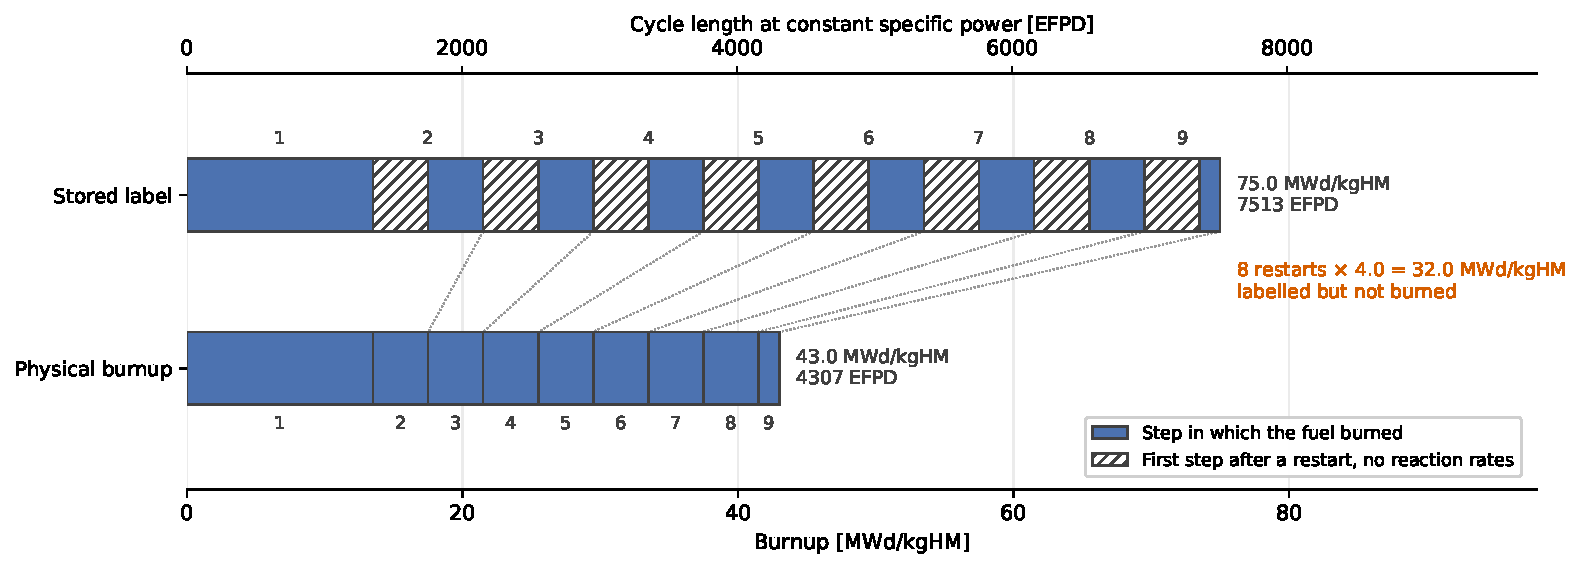
\includegraphics[width=\linewidth]{images/c5_restart_defect}
  \caption{Campaign 5, design C5-7: stored burnup against physical burnup.}
  \label{fig:c5-restart}
\end{figure}

\subsubsection{Campaign 6}
\label{sec:res-hist-c6}
%% labels of the Campaign section condensed here, kept so that the
%% cross-references of the other chapters still resolve
\label{sec:res-c5-c7}\label{sec:res-c6}\label{sec:res-c6-doe}\label{sec:res-c6-compare}

Campaign 6 applied the 4 corrections of
Section~\ref{sec:meth-campaigns} and executed 114 evaluations, 88 of them
feasible. The zoning lowered the median core peaking factor $F_{\Delta H}$ of the
design of experiments from 2.308 in Campaign 5 to 1.782, and one
design of the 114 reached the raised horizon, against 39 of 60 in
Campaign 5. The campaign then built the final form of the acquisition function
over its infill blocks, adding one element in each block
(Section~\ref{sec:res-c6-defects}):

\begin{itemize}
  \item \textbf{Bare uncertainty ranking:} the block returned 18 designs
        at a minimum normalised separation of 0.0007 from the designs
        already evaluated, so the batch-diversity threshold of
        Equation~\eqref{eq:batch-div} entered the next block.

  \item \textbf{Batch diversity:} the block returned 5 designs of 6
        above the upper reactivity bound while the constraint surrogate
        predicted all 6 feasible, so the feasibility margin of
        Equation~\eqref{eq:feas-margin} entered the block after it.

  \item \textbf{Feasibility margin:} the hypervolume, unchanged from its
        design-of-experiments value over the 2 blocks without the
        margin, increased by 22.7 per cent, and the acquisition function
        reached its final form.
\end{itemize}

Three studies on the evaluated designs of the campaign are kept in full in the
methodology:

\begin{itemize}
  \item \textbf{Search setting:} the NSGA-II search on the surrogates
        at $300\times400$, the setting whose seed-to-seed dispersion is
        negligible (Section~\ref{sec:res-c6-search}).

  \item \textbf{Axial leakage factor:} $L_\mathrm{ax} = 1.0289$, measured on 6 designs
        with a standard deviation of \SI{72}{pcm}
        (Section~\ref{sec:res-c6-lax}).

  \item \textbf{Derived upper reactivity bound:} $k_{\max} = 1.126$, from the smallest worth of the four regulating
        banks RE1 to RE4 inserted together, measured on 8 designs
        (Section~\ref{sec:res-c6-kmax}).
\end{itemize}

Every design between 13.8 and \SI{17.2}{wt\%} violated the upper
reactivity bound, and Campaign 7 narrowed the enrichment range to 3.0
to \SI{10.43}{wt\%}.

\subsubsection{Campaign 7}
\label{sec:res-hist-c7}
%% labels of the Campaign section condensed here, kept so that the
%% cross-references of the other chapters still resolve
\label{sec:res-c7-ctrl}\label{sec:res-c6-blocks}\label{tab:c6-blocks}\label{tab:c6-b2-collapse}\label{tab:c6-b3-fail}\label{fig:c6-convergence}\label{sec:res-c6-front}\label{fig:c6-front}\label{tab:c6-front}\label{fig:c6-parallel}\label{sec:res-c6-influence}\label{fig:c6-influence}\label{tab:c6-spearman}\label{fig:c6-constraints}\label{sec:res-c6-bscreen}\label{tab:c6-front-screened}\label{sec:res-c7}\label{sec:res-c7-basis}\label{eq:g-ctrl}\label{sec:res-c7-blocks}\label{tab:c7-blocks}\label{fig:c7-diversity}\label{tab:c7-nesting}\label{fig:c7-screens}\label{tab:c7-front}\label{fig:c7-pareto}\label{sec:res-c7-worth}\label{fig:c7-worth}\label{fig:c7-influence}\label{sec:res-c7-rodded}\label{fig:c7-rodded}\label{sec:res-c7-uncertainty}\label{fig:c7-histories}\label{fig:c7-uncertainty}\label{tab:c7-uncertainty}\label{sec:res-c7-hump}\label{fig:c7-khist-gd}\label{tab:c7-hump}\label{sec:res-c7-cost}\label{sec:res-c7-limits}

Campaign 7 added the measured controllability constraint of
Section~\ref{sec:meth-ctrl} to the loop, so that every evaluation also
solved the core with the four regulating banks inserted. Its 60
evaluations were executed without a failed case and give three results:

\begin{itemize}
  \item \textbf{Feasible designs and front:} 16 designs are feasible,
        and the front has 3 members, C7-48, C7-53 and C7-49.
  \item \textbf{Designs rejected by the derived bound:} 14 designs
        satisfied every constraint except the derived bound of 1.126,
        and all 14 were controllable, because their rodded
        multiplication factor did not exceed 0.99.
  \item \textbf{Effect of the derived bound on the front:} without the
        bound 3 of the 14 designs join the front, which then reaches a
        core peaking factor of 1.525 against 1.565 with the bound, so
        the derived bound removed the low-peaking end of the front
        (Figure~\ref{fig:c7-front-screen}).
\end{itemize}

Four designs reached the active batches with the Shannon entropy of
the fission source not yet converged, and all 4 are excluded from
every candidate list. The campaign was launched without the batch
diversity distance and executed its 3 infill blocks at
$\delta_\mathrm{min} = 0.05$, 2 of which collapsed, which was
identified only once it had finished.

Of the 60 designs of Campaign 7, 25 have a pitch below \SI{1.224}{cm},
at which the lattice cell truncates the guide-tube wall, and the pitch
is the design variable with the largest effect on the regulating-bank
worth. For these reasons Campaign 8 fixed the pitch at \SI{1.26}{cm}.
It also gave the 2 enrichment variables one value and applied the axial
leakage factor to $k_\mathrm{target}$.

\section{Campaign 8: maximum cycle length \texorpdfstring{$\mathrm{EFPD}$}{EFPD} and minimum radial peaking factor \texorpdfstring{$F_{\Delta H}$}{F dH}}
\sectionmark{Campaign 8: cycle length and peaking}
\label{sec:res-c8}

Campaign 8 is the last campaign of the original formulation of the
optimisation problem, which maximises the cycle length and minimises the core peaking factor, and
its front is the set of candidate cores of that formulation.

The campaign fixes the pitch at \SI{1.26}{cm}
(Section~\ref{sec:res-c8-intent}) and keeps the settings that the
earlier campaigns established:

\begin{itemize}
  \item The zoned loading map of Campaign 6
        (Section~\ref{sec:meth-zoning}).

  \item The measured controllability constraint of Campaign 7 as the
        binding constraint, with the derived bound of 1.166 behind it
        (Section~\ref{sec:meth-ctrl}).

  \item The axial leakage factor of Section~\ref{sec:res-c6-lax},
        applied to the end-of-cycle multiplication factor $k_\mathrm{target}$.
\end{itemize}

Every evaluation of the campaign also solves the beginning-of-life core
with only the first two regulating banks inserted and stores the resulting multiplication factor, which no earlier campaign computed.
Its post-analysis adds the three-dimensional core model, the boron worth
and the statistical significance of the front ordering
(Section~\ref{sec:res-c8-post}).

Every cycle length the campaign reports refers for the
first time in this work to a finite-height core, through the axially corrected $k_\mathrm{target}$ of Equation~\eqref{eq:ktarget-3d}. That value corrects the reactivity of the finite core and leaves the depletion
axially uniform.

\subsection{Specification}
\label{sec:res-c8-intent}

The design space, the fixed quantities and the transport settings are
those of Sections~\ref{sec:meth-c8-space} and~\ref{sec:meth-fidelity}.
\label{sec:res-c8-target}
The end-of-cycle criterion uses the axially corrected $k_\mathrm{target}$ of
Section~\ref{sec:meth-lax}, so the cycle lengths of this campaign are
finite-height values.
Table~\ref{tab:c8-target} compares it with the two-dimensional $k_\mathrm{target}$
of the earlier campaigns and gives its effect on the cycle length.

\begin{table}[htbp]
  \centering
  \small
  \caption{Campaign 8: $k_\mathrm{target}$ and its effect on the cycle length.}
  \label{tab:c8-target}
  \begin{tabular}{@{}lc@{}}
    \toprule
    Quantity & Value \\
    \midrule
    \multicolumn{2}{@{}l}{\emph{$k_\mathrm{target}$, mean over the 7 reflector thicknesses of its table}} \\
    Two-dimensional                      & 1.05256 \\
    Three-dimensional                    & 1.08298 \\
    Increase from the axial factor       & \SI{3040}{pcm} \\
    \addlinespace
    \multicolumn{2}{@{}l}{\emph{Three-dimensional $k_\mathrm{target}$ across the reflector range}} \\
    At $t_\mathrm{refl} = \SI{2.0}{cm}$  & 1.0839 \\
    At $t_\mathrm{refl} = \SI{5.66}{cm}$ & 1.0820 \\
    Variation                            & \SI{200}{pcm}, 0.3~MWd/kgHM, \SI{34}{EFPD} \\
    \addlinespace
    \multicolumn{2}{@{}l}{\emph{Ten designs whose depletion history crosses $k_\mathrm{target}$}} \\
    End-of-cycle slope [pcm per MWd/kgHM] & 552 to 756, median 652 \\
    Cycle shortening [EFPD]               & 403 to 552, median 468 \\
    \bottomrule
  \end{tabular}
\end{table}

The table shows two effects of the correction:

\begin{itemize}
  \item The reflector thickness is no longer a reactivity variable.
        Across its range $k_\mathrm{target}$ moves by about \SI{200}{pcm}, so in
        this campaign the reflector acts on the radial power shape alone.

  \item The depleting assembly stops earlier. The axial factor raises $k_\mathrm{target}$ by about \SI{3040}{pcm}, which moves the end of cycle
        of C8-29 from 35.5 to \SI{30.7}{MWd/kgHM}
        (Figure~\ref{fig:ktarget-3d-shift}) and shortens the cycle of the
        10 designs by 403 to \SI{552}{EFPD}. The longer cycles lose
        more, because the reactivity slope of the assembly flattens as
        the fuel depletes.
\end{itemize}

\begin{figure}[htbp]
  \centering
  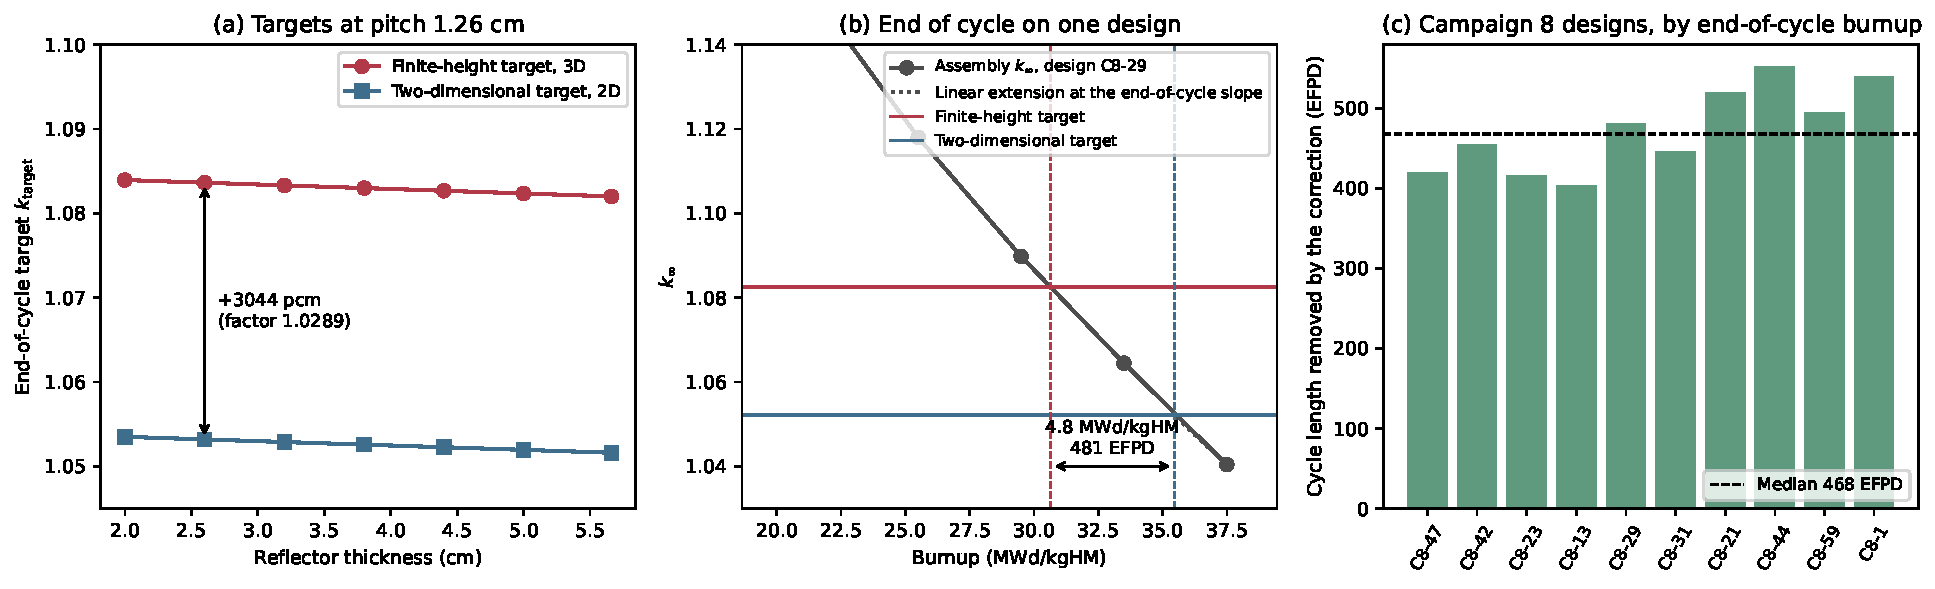
\includegraphics[width=\textwidth]{images/th_ktarget_3d_shift.pdf}
  \caption{Campaign 8: finite-height correction of $k_\mathrm{target}$.}
  \label{fig:ktarget-3d-shift}
\end{figure}

The pitch is fixed at \SI{1.26}{cm}, with two consequences:

\begin{itemize}
  \item The fixed pitch removes the defect of the guide-tube wall. Below
        \SI{1.224}{cm} the boundary of the lattice cell truncates the
        wall and replaces part of it by moderator, and 25 of the 60
        Campaign 7 designs, together with every earlier design at such a
        pitch, are reported subject to that defect.

  \item The fixed pitch costs part of the Campaign 7 front. Under the
        vessel fit of Campaign 7 the largest reflector at \SI{1.26}{cm}
        is \SI{12.75}{cm}, and 5 of the 6 designs on the
        controllability-constraint front, and 14 of the 60 in total,
        need a thicker one. Their low peaking relies on thick reflectors
        that fit only at a narrow pitch, so the lowest peaking factor expected of
Campaign 8 is near 1.60.
\end{itemize}

Three settings were declared before the campaign as the ones whose
effect it evaluates: the measured controllability constraint, the
two-bank reading computed and
stored but not constrained, and the acquisition settings
$\delta_\mathrm{min} = 0.14$ and $\kappa = 1.5$ of
Section~\ref{sec:meth-acq}, which Campaign 7 had executed at 0.05
and 1.0.

The campaign executed 60 evaluations on the workstation of
Table~\ref{tab:hosts} in \SI{21.02}{h}, all completed without error, at
\SI{1261}{s} per evaluation against \SI{949}{s} in Campaign 7. The
evaluator stores the time of every transport phase separately:

\begin{itemize}
  \item \textbf{Assembly solve:} \SI{11}{s}.

  \item \textbf{Core solve:} \SI{107}{s}.

  \item \textbf{Depletion:} \SI{925}{s}, the largest share, because the
        cycles are long, at 14.6 depletion steps per design against 13.0
        in Campaign 7.

  \item \textbf{Rodded solves:} \num{100} and \SI{102}{s} for the
        four-bank and the two-bank configuration.

  \item \textbf{Non-transport overhead:} the remaining \SI{16}{s}.
\end{itemize}

\subsection{Search}
\label{sec:res-c8-blocks}

Table~\ref{tab:c8-blocks} gives the 5 blocks, with the hypervolume
taken against the frozen reference of 1760 EFPD and 2.096, and the
spread of each variable given as its within-block range divided by its
range over all evaluated designs. Every infill block returned feasible
designs, moved at least 3 of the 4 variables and concentrated on the
long-cycle end of the feasible region, where the controllability
constraint binds. Block 1 moved 3 variables and kept the gadolinia
concentration fixed at \SI{8.0}{wt\%} in all its 6 designs, which is
the collapse mode of Campaign 7 limited to one variable.

\begin{table}[htbp]
  \centering
  \caption{Campaign 8: hypervolume and spread by block.}
  \label{tab:c8-blocks}
  \begin{tabular}{lccccccc}
    \toprule
    & & & & \multicolumn{4}{c}{Spread [--]} \\
    \cmidrule(l){5-8}
    Block & Designs & Feasible & Hypervolume (gain) & $e$ & $w_\mathrm{Gd}$ & $t_\mathrm{refl}$ & $n_\mathrm{Gd}$ \\
    \midrule
    DOE      & 36 & 9 & 1966.0             & 1.00 & 0.99 & 0.97 & 0.99 \\
    Infill 1 &  6 & 3 & 1966.0 (0.00\,\%)  & 0.50 & 0.00 & 0.33 & 0.86 \\
    Infill 2 &  6 & 3 & 2022.4 (+2.87\,\%) & 0.66 & 0.83 & 0.65 & 1.00 \\
    Infill 3 &  6 & 1 & 2022.4 (0.00\,\%)  & 0.69 & 0.68 & 0.26 & 1.00 \\
    Infill 4 &  6 & 3 & 2026.1 (+0.18\,\%) & 0.41 & 0.62 & 1.00 & 0.53 \\
    \bottomrule
  \end{tabular}
\end{table}

The convergence history is incomplete. The hypervolume gained
\SI{2.87}{\%} in block 2, then \SI{0.00}{\%} and \SI{0.18}{\%} in
blocks 3 and 4. The stopping rule of Section~\ref{sec:meth-loop-stop}
requires 3 consecutive gains below one per cent with no censored design
on the front, so the campaign is one block short of a formal stop.
Unlike the flat blocks of Campaign 7, blocks 3 and 4 are not
acquisition failures, for two reasons:

\begin{itemize}
  \item Their designs are diverse. Within the block, each variable spans 0.26 to 1.00 of its range over all evaluated designs (Table~\ref{tab:c8-blocks}).

  \item Their designs are at the controllability limit, where the
        surrogate expects the front to be. Of the 12, 11 have a
        rodded multiplication factor of 0.975 to 1.001, against the limit of 0.99
        (Figure~\ref{fig:c8-plane}(a)).
\end{itemize}

The campaign was stopped after infill 4 although the rule was not
satisfied. Each infill block was launched and analysed separately, and
after block 4, at the budget of 60 evaluations, the front was judged
sufficient for the post-analysis planned on its candidates, the
three-dimensional confirmation, the boron worth and the statistical significance of the
front ordering of Section~\ref{sec:res-c8-post}. The front is therefore
reported as the best available at that budget.

% ---------------------------------------------------------------------
%  Post-analysis of the Campaign 8 candidates.
%  Figures images/c8_post_*.pdf and tables tab:c8-post-* generated by
%  c8_post_figures.py from out_c8, boron_c8, confirm3d_c8_0ppm,
%  confirm3d_c8_dc37, confirm3d_c8_noparked and boron_c8_marginal.
% ---------------------------------------------------------------------

\subsection{Feasibility}
\label{sec:res-c8-screens}

Figure~\ref{fig:c8-plane} plots the 2 rodded configurations on the same
axes:

\begin{itemize}
  \item Panel (a), the four-bank configuration $k_\mathrm{RE}$ of
        Equation~\eqref{eq:k-re}, which carries the controllability
        constraint $g_\mathrm{ctrl} = k_\mathrm{RE} - 0.99 \le 0$ of
        Equation~\eqref{eq:g-ctrl-meth}.

  \item Panel (b), the two-bank configuration $k_\mathrm{RE12}$, with RE1 and
        RE2 inserted, whose value
        $g_\mathrm{ctrl,12} = k_\mathrm{RE12} - 0.99$ is computed and
        stored but not constrained.
\end{itemize}

\begin{figure}[htbp]
  \centering
  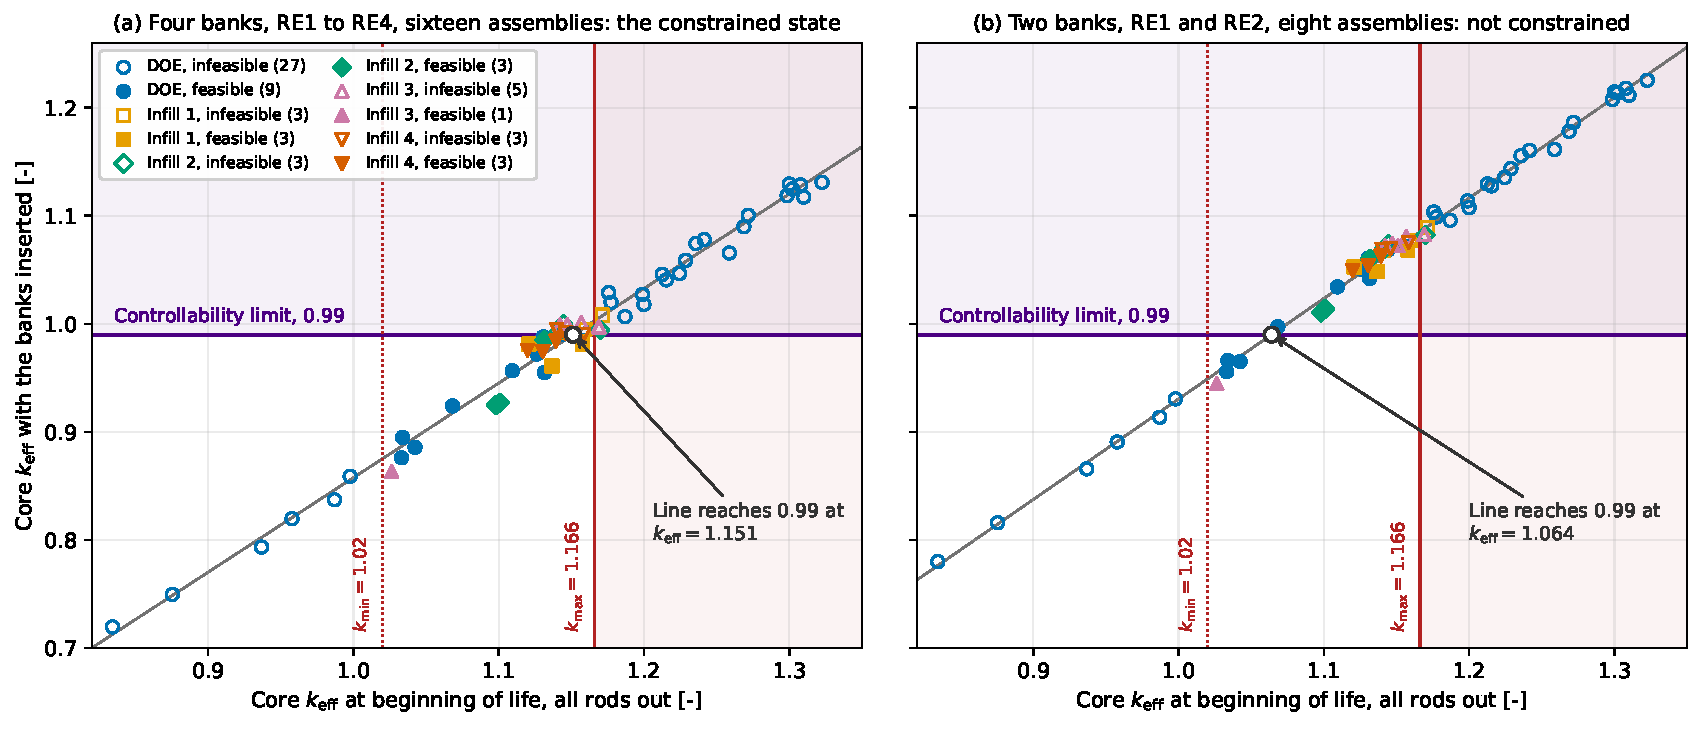
\includegraphics[width=\linewidth]{images/c8_ctrl_plane}
  \caption{Campaign 8: unrodded against rodded core multiplication factor.}
  \label{fig:c8-plane}
\end{figure}

A least-squares line through the 60 designs of
Figure~\ref{fig:c8-plane} reaches the controllability limit of 0.99 on
the rodded multiplication factor (Equation~\eqref{eq:g-ctrl-meth}) at an unrodded multiplication factor of 1.151 with the four regulating banks inserted and of
1.064 with RE1 and RE2. The residual standard deviations about the two
lines, 1059 and \SI{603}{pcm}, make each crossing the centre of an uncertainty interval rather than a
threshold. The four-bank crossing is below the derived
bound $k_{\max} = 1.166$, so a typical design that the bound rejects
already violates the controllability constraint.

Table~\ref{tab:c8-violations} counts, for each of the 6 constraints
of the campaign, the designs that violate it and the designs that
violate it alone. Of the 60 designs, 19 are feasible, 9 of them among
the 36 of the design of experiments, and no infeasible design violates
more than 2 constraints.

\begin{table}[!htb]
  \centering
  \small
  \caption{Campaign 8, 60 designs: designs that violate each constraint.}
  \label{tab:c8-violations}
  \begin{tabular}{@{}llcc@{}}
    \toprule
    Constraint & Definition & Violated by & Violated alone by \\
     &  & [designs] & [designs] \\
    \midrule
    Controllability $g_\mathrm{ctrl}$ & $k_\mathrm{RE} \le 0.99$ & 35 & 12 \\
    Upper reactivity bound $g_{k\max}$ & $k_\mathrm{eff}^\mathrm{core} \le 1.166$ & 23 & 0 \\
    Lower reactivity bound $g_{k\min}$ & $k_\mathrm{eff}^\mathrm{core} \ge 1.02$ & 6 & 6 \\
    Peaking bound $g_\mathrm{peak}$ & $F_{\Delta H} \le 2.0$ & 0 & 0 \\
    Enrichment limit $g_\mathrm{enr}$ & $e \le \SI{13.913}{wt\%}$ & 0 & 0 \\
    Vessel fit $g_\mathrm{geom}$ & Equation~\eqref{eq:ggeom} & 0 & 0 \\
    \midrule
    Feasible & all 6 satisfied & \multicolumn{2}{c}{19} \\
    \bottomrule
  \end{tabular}
\end{table}

Every one of the 23 designs that violate the upper reactivity bound
also violates the controllability constraint, whereas 12 designs
satisfy the bound and violate the constraint. The bound is therefore
redundant, and the controllability constraint is the binding one.

The constraint alone rejects 12 designs, the long-cycle designs from
3977 to \SI{6169}{EFPD}, whose rodded multiplication factor exceeds the
limit by 17 to \SI{1135}{pcm}. Two of them, C8-54 and C8-11, exceed it by
only 17 and \SI{63}{pcm}, about half and twice the standard deviation of
about \SI{30}{pcm} of a single core solve at the campaign setting, so
neither violation is established by one solve. Both were evaluated
again with 3 seeds (Table~\ref{tab:c8-rescore}).

\begin{table}[htbp]
  \centering
  \footnotesize
  \caption{Campaign 8, designs C8-54 and C8-11: controllability constraint with 3 seeds.}
  \label{tab:c8-rescore}
  \begin{tabular}{@{}lcccccccl@{}}
    \toprule
    Design & EFPD & $F_{\Delta H}$ & \multicolumn{2}{c}{Campaign, one seed} &
      \multicolumn{2}{c}{Re-score, 3 seeds} & Dominated by \\
    \cmidrule(lr){4-5}\cmidrule(lr){6-7}
     & [d] & [--] & $k_\mathrm{RE}$ & [pcm] & $k_\mathrm{RE}$ & [pcm] & \\
    \midrule
    C8-54 & 3977 & 1.615 & 0.99017 & $+17$ & $0.99038 \pm 0.00054$ & $+38 \pm 54$ & C8-21, C8-44 \\
    C8-11 & 4835 & 1.613 & 0.99063 & $+63$ & $0.99053 \pm 0.00025$ & $+53 \pm 25$ & C8-44 \\
    \bottomrule
  \end{tabular}
\end{table}

Both designs remain above the constraint value after the re-score, so
the feasibility count stays at 19, and both are dominated on the
objectives, so the front is unchanged either way.

Table~\ref{tab:c8-worth} gives the bank worths of
Equation~\eqref{eq:bank-worth} over the 60 designs and the upper
reactivity bounds $k_{\max}$ that Equation~\eqref{eq:k-max-derived}
derives from them, as the four-bank bound of Campaign 7 was derived in
Section~\ref{sec:res-c6-kmax}. The table supports three results:

\begin{itemize}
  \item \textbf{Dependence of the worth:} the pitch is fixed at
        \SI{1.26}{cm}, so the worth varies only with the 4 design
        variables. The enrichment governs both worths, with a correlation
        of $-0.95$, and the gadolinia rod count has a weaker effect,
        $-0.28$ and $-0.36$. The ratio of the two-bank to the four-bank
        worth is 0.434 to 0.471, with a mean of 0.458.

  \item \textbf{Derived bound $k_{\max}$:} Equation~\eqref{eq:k-max-derived}
        takes the smallest worth over all evaluated designs, so every design below
        the resulting bound, 1.119 for four banks and 1.046 for two, is
        compensated by the banks whatever its own worth.

  \item \textbf{Typical bound $\tilde{k}_{\max}$:} the median worth in
        place of the smallest gives the upper reactivity bound of a
        typical design, 1.148 for four banks and 1.057 for two, and
        defines the window above the lower reactivity bound of 1.02.
        That window is about \SI{12800}{pcm} wide for four banks and
        \SI{3700}{pcm} for two, and the two-bank window holds 4 of
        the 19 feasible designs.
\end{itemize}

\begin{table}[htbp]
  \centering
  \small
  \caption{Campaign 8, 60 designs: regulating-bank worth and the upper reactivity bound.}
  \label{tab:c8-worth}
  \begin{tabular}{@{}lcc@{}}
    \toprule
    Quantity & Four banks & Two banks \\
    \midrule
    Worth [pcm]                        & \num{11626} to \num{19294} & \num{5404} to \num{8753} \\
    Median worth [pcm]                 & \num{13860}                & \num{6390} \\
    Ratio to the four-bank worth [--]  & --                         & 0.434 to 0.471 \\
    \addlinespace
    Correlation with $e$ [--]          & $-0.95$                    & $-0.95$ \\
    Correlation with $n_\mathrm{Gd}$ [--] & $-0.28$                 & $-0.36$ \\
    \addlinespace
    $k_{\max}$ [--]                    & 1.119                      & 1.046 \\
    $\tilde{k}_{\max}$ [--]            & 1.148                      & 1.057 \\
    Window from 1.02 to $\tilde{k}_{\max}$ [pcm] & \num{12800}      & \num{3700} \\
    Feasible designs retained          & 19 of 19                   & 4 of 19 \\
    \bottomrule
  \end{tabular}
\end{table}

\subsection{Pareto front}
\label{sec:res-c8-front}

The feasible non-dominated set holds 8 designs, from 1941 to 5782
EFPD and from $F_{\Delta H}$ 1.510 to 1.677. Table~\ref{tab:c8-front}
lists them and Figure~\ref{fig:c8-pareto} places every design in the
objective plane with its block. In the table the ring enrichments are
the as-built centre, middle and periphery values, the excess is the
beginning-of-life reactivity at \SI{1000}{ppm} that the rods must hold,
and the peaking factor is given with all rods out ($F$), with two banks
in ($F_2$) and with four banks in ($F_4$).

Figure~\ref{fig:c8-pareto} shows that 4 front designs come from the
design of experiments, 3 from infill block 2 and one from block 4.
The discharge-burnup limit of \SI{55}{MWd/kgHM} of
Section~\ref{sec:meth-atf} removes design C8-1, the longest cycle of the front, at an end-of-cycle burnup
of \SI{57.7}{MWd/kgHM}. The reduced front ends at design C8-59, at
\num{5104} effective full power days and \SI{51.0}{MWd/kgHM}, and no
design is censored.

\begin{table}[htbp]
  \centering
  \small
  \caption{Campaign 8: Pareto front.}
  \label{tab:c8-front}
  \setlength{\tabcolsep}{3.4pt}
  \begin{tabular}{ccccccccccc}
    \toprule
    Design & EFPD & rings & $w_\mathrm{Gd}$ & $n_\mathrm{Gd}$ &
      $t_\mathrm{refl}$ & $k^\mathrm{core}$ & excess & $F$ & $F_{2}$ &
      $F_{4}$ \\
    {[--]} & [d] & [wt\%] & [wt\%] & [rods] & [cm] & [--] & [pcm] &
      [--] & [--] & [--] \\
    \midrule
    C8-47 & 1941 & 3.16, 3.93, 5.05  & 2.88 & 12 & 4.29 & 1.098 &  8930 & 1.510 & 1.991 & 2.314 \\
    C8-42 & 1968 & 3.20, 3.97, 5.11  & 2.88 & 12 & 3.76 & 1.101 &  9154 & 1.522 & 1.997 & 2.264 \\
    C8-23 & 2346 & 3.56, 4.42, 5.68  & 2.80 & 12 & 4.81 & 1.132 & 11626 & 1.534 & 1.968 & 2.356 \\
    C8-29 & 3070 & 4.25, 5.27, 6.79  & 0.18 & 40 & 4.69 & 1.158 & 13627 & 1.542 & 1.935 & 2.218 \\
    C8-21 & 4221 & 5.63, 6.98, 8.99  & 3.11 & 32 & 4.92 & 1.126 & 11220 & 1.592 & 1.934 & 2.194 \\
    C8-44 & 5019 & 6.65, 8.25, 10.61 & 3.20 & 40 & 5.33 & 1.132 & 11631 & 1.612 & 1.996 & 2.177 \\
    C8-59 & 5104 & 6.73, 8.35, 10.75 & 4.32 & 40 & 5.66 & 1.120 & 10701 & 1.634 & 1.998 & 2.214 \\
     C8-1 & 5782 & 7.94, 9.85, 12.68 & 7.43 & 40 & 3.94 & 1.131 & 11554 & 1.677 & 2.007 & 2.210 \\
    \bottomrule
  \end{tabular}
\end{table}

\begin{figure}[htbp]
  \centering
  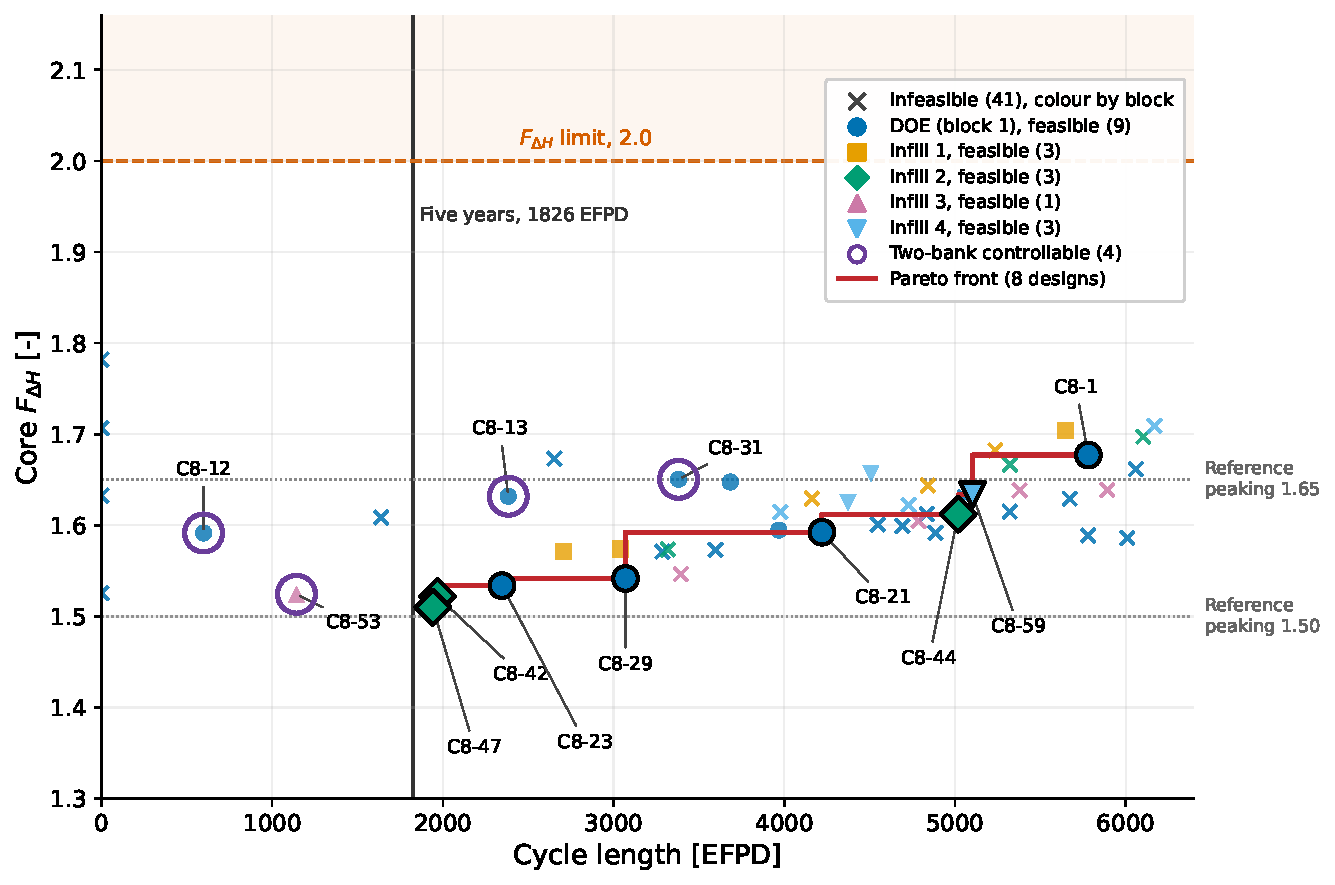
\includegraphics[width=0.85\linewidth]{images/c8_pareto}
  \caption{Campaign 8: objective space by block.}
  \label{fig:c8-pareto}
\end{figure}

Three features of the front govern the candidate selection:

\begin{enumerate}
  \item \textbf{Lowest peaking factor:} it did not rise on the front as
        expected. Before the campaign was executed, it was
        expected near 1.60, because the lowest-peaking designs of
        Campaign 7 owed their low peaking to thick reflectors, which do
        not fit at the fixed pitch of \SI{1.26}{cm}
        (Section~\ref{sec:res-c8-intent}). The lowest value of
        Campaign 8 is 1.510, at design C8-47, which reaches it without a
        thick reflector. Its reflector is \SI{4.29}{cm}, and its
        low peaking comes from a low enrichment, 3.16 to
        \SI{5.05}{wt\%} over the three rings, with 12 poisoned pins
        and a short cycle of \SI{1941}{EFPD}. Over the 19 feasible designs the enrichment ranges
        from 3.45 to \SI{11.03}{wt\%} and the core peaking factor from
        1.510 to 1.705, and the designs with the lower enrichment have
        the lower peaking factor. The Pearson correlation coefficient
        between the two is $+0.82$, where $+1$ would mean that the
        peaking factor increases linearly with the enrichment.

  \item \textbf{Controllability margin:} every front design is close
        to the controllability limit. The unrodded multiplication factors range from 1.098 to 1.158, and the rodded ones from 0.925 to 0.988,
        so the beginning-of-life excess that the four banks must hold is
        between \num{8930} and \SI{13627}{pcm} with the soluble boron
        already in the coolant. Design C8-29, with \SI{0.18}{wt\%}
        gadolinia on 40 pins, is effectively unpoisoned and has the
        largest excess. Every front design needs all four banks, since
        with the first two alone its multiplication factor is 1.011 to 1.071. The 4 two-bank controllable designs, C8-12, C8-53, C8-13 and
        C8-31, are kept at 0.945 to 0.966 by the first two banks alone
        (Figure~\ref{fig:c8-split}(a)).

  \item \textbf{Rodded peaking:} the two-bank peaking of every front
        design is 1.93 to 2.01. With only RE1 and RE2 inserted the front
        is at the peaking limit, and with all four banks it exceeds the
        limit by 0.18 to 0.36 (Figure~\ref{fig:c8-split}(b)). Over all 60
        designs the two-bank peaking of the two-dimensional core is
        1.82 to 2.35, above the unrodded 1.51 to 1.78 for every design, because the regulating
        banks are in the central assemblies and their insertion moves
        the power towards the periphery. The rodded peaking still depends on the
        design. Its standard deviation, 0.097, is twice that of the
        unrodded peaking, 0.052, and it decreases as the enrichment increases,
        at a correlation of $-0.61$.
\end{enumerate}

\begin{figure}[htbp]
  \centering
  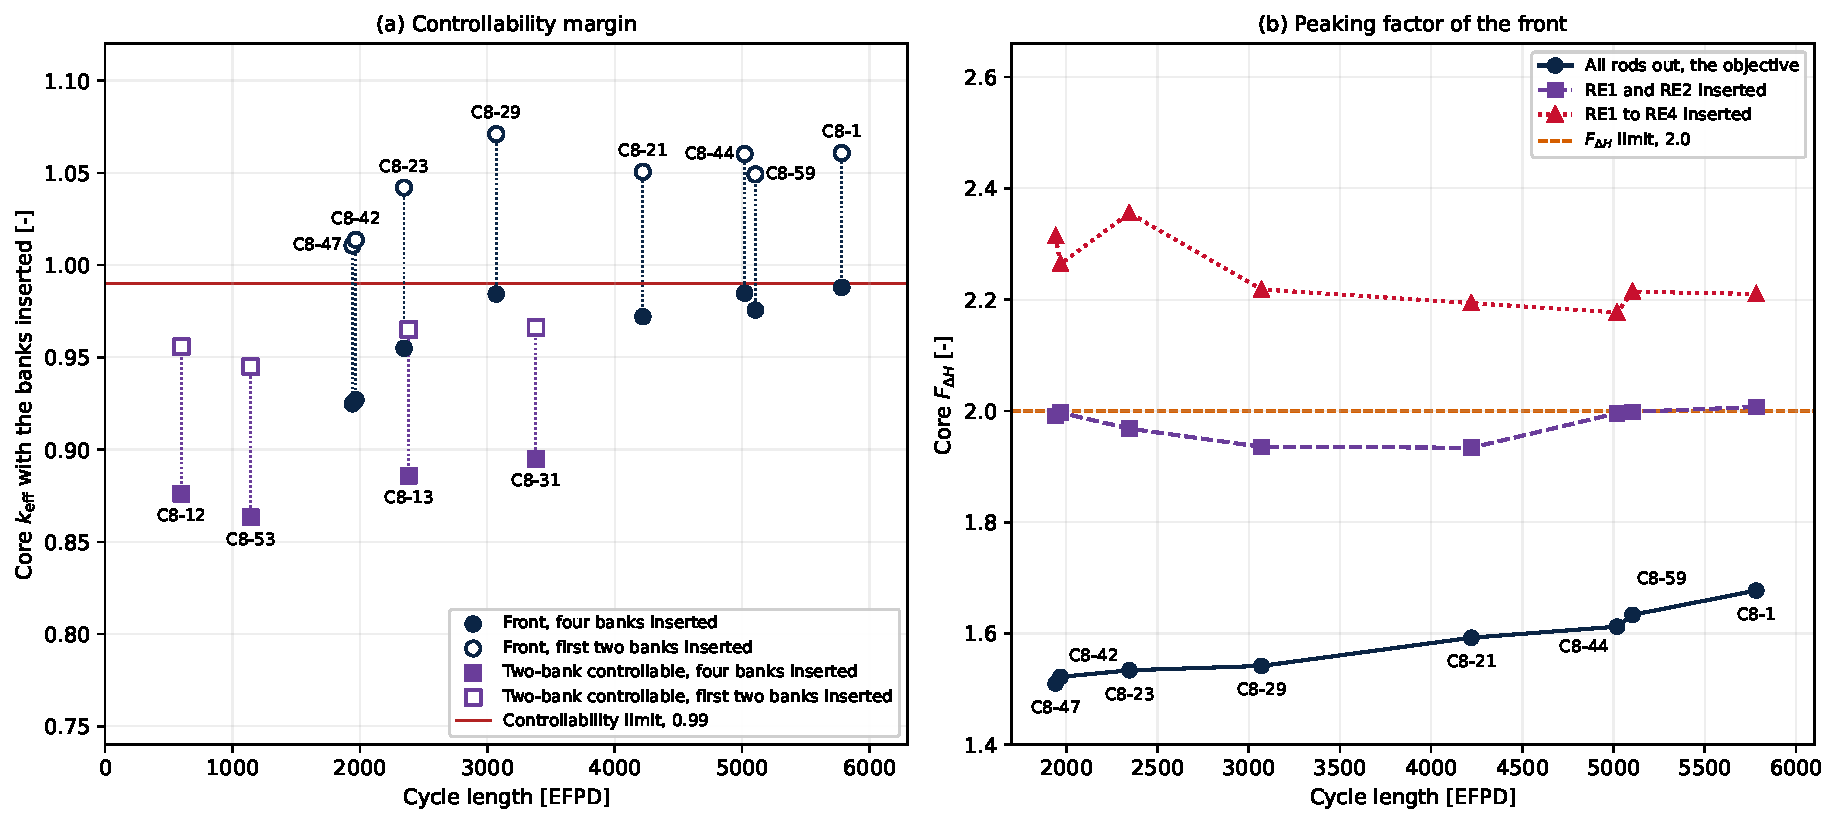
\includegraphics[width=0.95\linewidth]{images/c8_front_split}
    \caption{Campaign 8: front and two-bank designs. (a)~Rodded multiplication factor. (b)~Peaking factor in 3 rod configurations.}
  \label{fig:c8-split}
\end{figure}

\label{sec:res-c8-mission}
The reported refuelling interval of 5 years corresponds to
\SI{1826}{EFPD}. Against that interval the Campaign 8 designs divide into
three groups:

\begin{itemize}
  \item \textbf{Front:} every design satisfies the interval, C8-47 with a
        margin of \SI{115}{EFPD} and C8-1 by a factor of 3.2.

  \item \textbf{Two-bank designs:} C8-13 and C8-31 satisfy the
        interval, and C8-53, at \SI{1142}{EFPD}, is \SI{684}{EFPD} short
        of it.
\end{itemize}

The enrichments reported for LABGENE can be placed against the same
cycle lengths. The 6 to \SI{8}{wt\%} stated in
2014~\cite{dinizcosta_2017} corresponds to designs C8-31 and C8-21, at
3381 and \SI{4221}{EFPD}.

Two effects of the model act on these cycle lengths, and both make the
comparison conservative:

\begin{itemize}
  \item \textbf{Fixed boron concentration:} the depletion keeps
        \SI{1000}{ppm} for the whole cycle, so every cycle length is a
        lower bound for a core operated at its critical boron
        concentration, which is diluted as the fuel depletes.

  \item \textbf{Burnup dependence of the leakage factor:} it increases
        the 6 longest cycles by 11 to \SI{56}{d}
        (Section~\ref{sec:res-kt-burnup}).

\end{itemize}

Maximising the cycle length moves every front design beyond the
reported interval and, through the excess reactivity it requires,
towards the controllability limit. The cycle length is therefore not
the binding requirement of this core, while controllability and peaking
are, so the cycle length belongs among the constraints, at the required
value. These observations led to the reformulation of the optimisation
problem applied in Campaign 9 (Section~\ref{sec:res-c9}).

\subsection{Validation of the framework}
\label{sec:res-c8-validation}
\label{tab:c8-cv-loo}\label{fig:c8-cv-loo}\label{fig:c8-cv-walkforward}\label{tab:c8-front-stability}\label{fig:c8-stab-chrono}\label{fig:c8-stab-robust}

This section applies the 2 tests of
Section~\ref{sec:validation-framework} to the method of Campaign 8
before the candidates are selected, to the surrogate and to the
stability of the front under the Monte Carlo noise, to separate the
results that come from the physics of the model from those that
depend on an approximation of the method.

\subsubsection{Validation of the surrogate}
\label{sec:res-c8-cv}
The Gaussian-process surrogates are tested by leave-one-out
cross-validation, in which each evaluated design is held out once and
predicted from the other 59, and by walk-forward validation, in which
the surrogates trained on the evaluations completed before each infill
block predict the designs of that block.
Table~\ref{tab:c8-val-surrogate} gives the results in the four
measures of Section~\ref{sec:validation-surrogate}, the coefficient of
determination $R^2$, the root-mean-square error, the Spearman rank
correlation $\rho_\mathrm{S}$ and the two-sigma coverage, which is
0.954 for a calibrated Gaussian predictor.

\begin{table}[htbp]
  \centering
  \small
  \caption{Campaign 8: validation of the surrogate.}
  \label{tab:c8-val-surrogate}\label{tab:c8-validation}
  \begin{tabularx}{\textwidth}{@{}>{\raggedright\arraybackslash}p{0.42\textwidth}>{\raggedright\arraybackslash}X@{}}
    \toprule
    Quantity & Result \\
    \midrule
    LOOCV, cycle length & $R^2 = 0.988$, RMSE \SI{220}{EFPD}, $\rho_\mathrm{S} = 0.997$ \\
    LOOCV, $F_{\Delta H}$ & $R^2 = 0.690$, RMSE 0.029, $\rho_\mathrm{S} = 0.830$ \\
    LOOCV, $k_\mathrm{eff}^\mathrm{core}$ and $k_\mathrm{RE}$ & $R^2 = 0.978$ and 0.985, two-sigma coverage 0.97 \\
    Walk-forward RMSE of the cycle length, blocks 1 to 4 & 285, 191, 136, \SI{107}{EFPD} \\
    \bottomrule
  \end{tabularx}
\end{table}

The cycle length is the best predicted quantity and the peaking factor
the worst. The predictive intervals of the objectives are too narrow,
with a standard deviation of the standardised residual,
$s_z$ of Equation~\eqref{eq:val-sz}, of 1.26 to 1.63 against 1 for a
calibrated predictor. The surrogates of the two constraint
multiplication factors order the designs almost exactly and give
calibrated uncertainties (rank correlation above 0.96), so they predict
reliably whether a design satisfies the reactivity window and the
controllability constraint.

The coverage of the constraints decides whether the feasibility margin
of Equation~\eqref{eq:feas-margin} worked as intended. That margin
admits a candidate only if its predicted constraint value plus $\kappa$
predictive standard deviations is negative, so it is as safe as
intended only if those standard deviations are not too small. The
coverage of 0.97 is above the nominal 0.954, so the predictive
standard deviations of the constraints are not underestimated, and the
margin applied during the campaign was at least as wide as intended.

The walk-forward test measures how the surrogate improved during the
campaign. Infill block 1, predicted from the 36 designs of the design
of experiments, has an error of \SI{285}{EFPD} on the cycle length,
and block 4, predicted from the 54 designs evaluated before it,
\SI{107}{EFPD}, so the surrogate that selected each block was more
accurate as the training data grew from 36 to 54 evaluations.

\subsubsection{Validation of the front}
\label{sec:res-c8-stability}

The front is tested against the Monte Carlo noise of the transport
solves, and that noise is measured first, from 14 pairs of core
solves with 2 seeds, in two and in three dimensions, at \num{150000}
particles and 200 batches, 80 of them inactive. Table~\ref{tab:c8-post-sigma} gives the
seed-to-seed standard deviations. That of the multiplication factor, 14 to
\SI{24}{pcm}, is not larger than the 20 to \SI{28}{pcm} that each solve
reports, so the reported uncertainty does not underestimate the
seed-to-seed dispersion. That of the peaking factor is 0.011 to 0.012
with all rods out, about 0.014 when scaled to the campaign fidelity of
$100\,000 \times 170$.

\begin{table}[htbp]
  \centering
  \footnotesize
  \caption{Campaign 8 designs, all rods out: seed-to-seed standard deviation of the core solves.}
  \label{tab:c8-post-sigma}
  \begin{tabular}{@{}l l r r r@{}}
    \toprule
    Configuration & Model & pairs & $\sigma_\mathrm{seed}(k)$, pcm & $\sigma_\mathrm{seed}(F_{\Delta H})$ \\
    \midrule
    ARO, 1000 ppm & 2D & 14 & 14 & 0.0106 \\
    ARO, 1000 ppm & 3D & 14 & 24 & 0.0119 \\
    \bottomrule
  \end{tabular}
\end{table}

Each of 5000 replicates perturbs the objectives of every feasible
design by Gaussian noise of that size, $\sigma_F = 0.014$ on the peaking
factor and the cycle-length noise of Equation~\eqref{eq:val-sigma-cycle}
on the cycle length, and recomputes the non-dominated set. The
Pareto-membership frequency of a design is the fraction of replicates
in which it stays on the front, 1 when it always does.
Table~\ref{tab:c8-val-front} gives it for the 8 members.

\begin{table}[htbp]
  \centering
  \small
  \caption{Campaign 8: Pareto-membership frequency of the front members under noise.}
  \label{tab:c8-val-front}
  \begin{tabular}{@{}lcccccccc@{}}
    \toprule
    Design & C8-47 & C8-42 & C8-23 & C8-29 & C8-21 & C8-44 & C8-59 & C8-1 \\
    \midrule
    Frequency [--] & 0.69 & 0.63 & 0.67 & 0.99 & 0.81 & 0.86 & 0.98 & 1.00 \\
    \bottomrule
  \end{tabular}
\end{table}

The front is stable under the transport noise except at its
low-peaking end, where the order of C8-47, C8-42 and C8-23 is not
statistically significant. Their peaking factors differ by less than
one standard deviation between neighbours, so ranking them by
$F_{\Delta H}$ would require at least 4 seeds per design. The front was
also still growing when the campaign stopped, since C8-59 joined it at
the last evaluation.

\section{Post-analysis of Campaign 8}
\label{sec:res-c8-post}

The post-analysis of Campaign 8 examines the 11 designs
of interest, the 8 front members and the two-bank designs C8-53,
C8-13 and C8-31, under the readings that the campaign evaluation does not give:

\begin{itemize}
\item \textbf{Boron worth, mid-cycle hump and MTC boron limit
        (Section~\ref{sec:res-c8-boron}):} the 11 designs re-solved
        between 0 and \SI{1500}{ppm} in the 3 rod configurations on
        the two-dimensional core, one seed, 132 solves, with the hump read from the depletion histories stored by the evaluator, and the moderator
        temperature coefficient of C8-47 at two primary conditions on
        the two- and on the three-dimensional model.

\item \textbf{Two-bank control in three dimensions
        (Section~\ref{sec:res-c8-split}):} the 11 designs re-solved
        on the three-dimensional core model at \SI{1000}{ppm} in the
        3 rod configurations, with 2 seeds.

\item \textbf{Leakage factors of $k_\mathrm{target}$
        (Section~\ref{sec:res-kt-burnup}):} the two factors:
        \begin{itemize}
          \item The radial factor over burnup, fuel loading, reflector
                thickness and pitch, on depleted assembly and core solves
                of 10 designs with 3 seeds and on 42 solves of the
                reference assembly.
          \item The axial factor over rod configuration, withdrawn rods
                and downcomer, on the three-dimensional core model.
        \end{itemize}
\end{itemize}

The candidate decision closes the section.

\subsection{Boron worth, critical concentration and the MTC boron limit}
\label{sec:res-c8-boron}

Every campaign holds the soluble boron at \SI{1000}{ppm} from beginning
of life through the whole depletion (Section~\ref{sec:meth-boron}), and
the controllability constraint is evaluated at beginning of life, so the campaign evaluation gives neither the concentration that each design needs to
control its excess reactivity nor the reactivity that a design with
residual gadolinium gains as the absorber burns out. The 11 designs
were therefore re-solved between 0 and \SI{1500}{ppm}, unrodded and
with the regulating banks inserted, on the two-dimensional core with
one seed at $150\,000\times200$. At \SI{1000}{ppm} the multiplication factors of these solves reproduce the campaign values within $-72$ to \SI{+50}{pcm} over 33 comparisons. Together with the depletion history of each design stored by the evaluator, the solves give five quantities:

\begin{itemize}
  \item \textbf{Differential boron worth $W_\mathrm{B}$:} the
        reactivity worth of one ppm of boron, averaged between 0 and
        \SI{1000}{ppm}. The worth between 1000 and \SI{1500}{ppm} is the one
        with which the critical concentration is projected from the
        solve at \SI{1000}{ppm}.
  \item \textbf{Subcriticality margin $M_8(1000)$:} the reactivity by
        which the core is subcritical, positive when subcritical, with
        the 8 assemblies of banks RE1 and RE2 inserted at
        \SI{1000}{ppm}.
  \item \textbf{Two-bank concentration $c_8$:} the least boron with
        which banks RE1 and RE2 alone keep the core at $k \le 0.99$,
        the margin of Equation~\eqref{eq:g-ctrl-meth}.
  \item \textbf{Hump $\Delta\rho_\mathrm{hump}$ and burnup
        $B_\mathrm{peak}$:} the reactivity of the most reactive
        operating point after beginning of life minus that of beginning
        of life, Equation~\eqref{eq:c7-hump}, from the assembly
        depletion of the campaign, and the burnup of that point.
  \item \textbf{Critical concentrations $c_\mathrm{BOL}$ and
        $c_\mathrm{peak}$:} the boron at which the unrodded core is
        critical, at beginning of life and at the most reactive
        operating point, both extrapolated linearly from the unrodded
        solve at \SI{1000}{ppm}.
\end{itemize}

The critical concentrations of Campaign 8 are the linear predecessor
of Equation~\eqref{eq:c9-cmax}. The beginning-of-life concentration is
projected from the solve at \SI{1000}{ppm} with the worth measured
between 1000 and \SI{1500}{ppm}, and the hump term, converted to the
core by the radial leakage factor of Equation~\eqref{eq:ktarget} and
set to zero when negative, is divided by the same worth. The estimate
assumes that the worth stays constant above \SI{1500}{ppm}. For design
C8-47 the concentration found by root finding is \SI{2327}{ppm},
against the estimate of \SI{2348}{ppm}. Table~\ref{tab:c8-post-boron}
gives the five quantities for the 11 designs.

\begin{table}[htbp]
  \centering
  \small
  \begin{threeparttable}
  \caption{Campaign 8 designs: boron worth, two-bank margin, mid-cycle hump and critical boron concentration.}
  \label{tab:c8-post-boron}
  \setlength{\tabcolsep}{3.6pt}
  \begin{tabular}{@{}ccccccccc@{}}
    \toprule
    Design & $e$ & $W_\mathrm{B}$ & $M_8(1000)$\tnote{a} & $c_8$\tnote{b} &
      $B_\mathrm{peak}$ & $\Delta\rho_\mathrm{hump}$ & $c_\mathrm{BOL}$ &
      $c_\mathrm{peak}$ \\
    {[--]} & [wt\%] & [pcm/ppm] & [pcm] & [ppm] & [MWd/kgHM] & [pcm] &
      [ppm] & [ppm] \\
    \midrule
    C8-53 & 3.45  & 8.54 & 5867    & 415  & 7.5  & $-676$  & 1312 & 1312 \\
    C8-47 & 4.39  & 6.98 & $-1053$ & 1316 & 0.5  & $-1591$ & 2348 & 2348 \\
    C8-42 & 4.44  & 6.88 & $-1287$ & 1352 & 0.5  & $-1578$ & 2377 & 2377 \\
    C8-23 & 4.94  & 6.31 & $-4068$ & 1861 & 0.5  & $-1356$ & 2979 & 2979 \\
    C8-13 & 5.14  & 6.14 & 3581    & 566  & --   & $-723$  & 1697 & 1697 \\
    C8-29 & 5.90  & 5.22 & $-6643$ & 2539 & 1.5  & $+2822$ & 3677 & 4277 \\
    C8-31 & 6.59  & 4.79 & 3455    & 472  & 17.5 & $+4580$ & 1701 & 2760 \\
    C8-21 & 7.81  & 4.18 & $-4783$ & 2499 & 17.5 & $+1295$ & 3752 & 4095 \\
    C8-44 & 9.23  & 3.50 & $-5678$ & 2895 & 17.5 & $+1812$ & 4372 & 4940 \\
    C8-59 & 9.34  & 3.54 & $-4677$ & 2709 & 21.5 & $+1150$ & 4112 & 4473 \\
    C8-1  & 11.03 & 3.13 & $-5764$ & 3302 & 0.5  & $-626$  & 4674 & 4674 \\
    \bottomrule
  \end{tabular}
  \begin{tablenotes}[flushleft]\footnotesize
    \item[a] Banks RE1 and RE2, \SI{1000}{ppm}, two-dimensional core, one seed.
    \item[b] Values above \SI{1500}{ppm} are extrapolated.
  \end{tablenotes}
  \end{threeparttable}
\end{table}

The table and Figure~\ref{fig:c8-hump}, which shows the reactivity
history of each design relative to beginning of life, support 4
readings:

\begin{itemize}
  \item \textbf{Boron worth:} it decreases with enrichment, from 8.54
        to \SI{3.13}{pcm} per ppm, and at \SI{1000}{ppm} the boron
        provides 20 to 32 per cent of the compensation of the
        beginning-of-life excess reactivity, the four regulating banks
        the rest.
  \item \textbf{Two-bank concentration:} the two-bank designs reach the
        two-bank constraint at 415 to \SI{566}{ppm}, C8-47 and C8-42 at
        1316 and \SI{1352}{ppm}, and the other 6 front designs need
        1861 to \SI{3302}{ppm}, all by extrapolation.
  \item \textbf{Positive hump, panel (a):} 5 designs gain $+1150$ to
        \SI{+4580}{pcm} over beginning of life at 1.5 to
        \SI{21.5}{MWd/kgHM} as the gadolinium burns out, which raises
        their critical boron concentration by 343 to \SI{1059}{ppm}
        once converted to the core by the radial leakage factor and
        divided by their boron worth.
  \item \textbf{Beginning of life most reactive, panel (b):} for 6
        designs the reactivity never returns to its beginning-of-life
        value, their hump is $-626$ to \SI{-1591}{pcm}, and
        $c_\mathrm{peak} = c_\mathrm{BOL}$.
\end{itemize}

The hump is not ordered by enrichment. The largest, \SI{+4580}{pcm},
belongs to C8-31 at \SI{6.59}{wt\%}, while the reactivity of C8-1, at
\SI{11.03}{wt\%}, stays below its beginning-of-life value.

\begin{figure}[!htb]
  \centering
  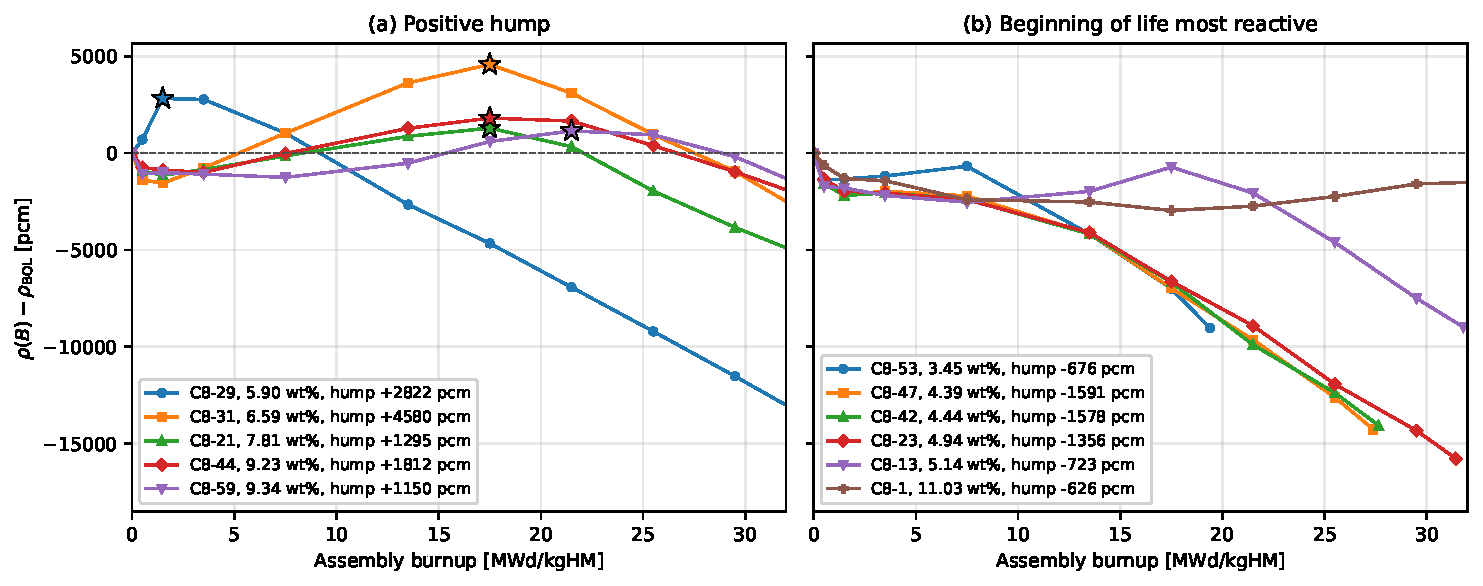
\includegraphics[width=\textwidth]{images/c8_hump_histories}
    \caption{Campaign 8 designs: assembly reactivity relative to beginning of life against burnup.}
  \label{fig:c8-hump}
\end{figure}

\label{sec:res-c8-mtc}
The critical concentrations of Table~\ref{tab:c8-post-boron} are the
boron that each design needs at power, and that boron has an upper
limit, the MTC boron limit $c_\mathrm{MTC}$ of
Equation~\eqref{eq:ceiling}. Because this limit depends on the lattice,
it was measured on the lattice of the recommended design, C8-47, with
the scan of Section~\ref{sec:meth-mtc} at the two primary conditions,
on the two-dimensional core and on the three-dimensional core model.
Table~\ref{tab:c8-mtc} gives the limits, each the root of the weighted
straight-line fit of the coefficient over the 3 scanned
concentrations nearest the sign change.

\begin{table}[htbp]
  \centering
  \small
    \begin{threeparttable}
  \caption{Campaign 8, design C8-47, zoned core: MTC boron limit at two primary conditions.}
  \label{tab:c8-mtc}
  \begin{tabular}{@{}rcrrr@{}}
    \toprule
    Pressure & Temperatures & 2D limit & 3D result & 3D margin on 2327\,ppm \\
    {[MPa]} & [K] & [ppm] & [ppm] & [ppm] \\
    \midrule
    15.5 & 570 to 590 & $2334 \pm 60$  & $3008 \pm 70$ & $+681$ \\
    12.8 & 547 to 567 & $2174 \pm 100$ & $2758 \pm 75$ & $+431$ \\
    \bottomrule
  \end{tabular}
  \end{threeparttable}
\end{table}

Two checks support the scan:

\begin{itemize}
  \item \textbf{Fuel temperature coefficient:} computed at the lowest
        concentration between 600, 900 and \SI{1200}{K}, it is negative
        and statistically significant throughout, $-2.15$ to
        \SI{-1.79}{pcm} per K at \SI{15.5}{MPa} and $-2.08$ to
        \SI{-1.85}{pcm} per K at \SI{12.8}{MPa}, so the temperature
        treatment of the cross sections is correct.
  \item \textbf{Axial leakage term of
        Equation~\eqref{eq:axial-feedback}:} it is
        $-10.63 \pm \SI{0.55}{pcm}$ per K, 29 per cent of the
        coefficient of the three-dimensional core, and it raises the
        limit by $674 \pm \SI{92}{ppm}$ at \SI{15.5}{MPa} and by
        $584 \pm \SI{125}{ppm}$ at \SI{12.8}{MPa}, the difference
        between the 2D and 3D columns of Table~\ref{tab:c8-mtc}, so the
        two-dimensional limit is a conservative bound.
\end{itemize}

C8-47 needs \SI{2327}{ppm} at beginning of life, the root of the
reactivity curve of its zoned core at \SI{570}{K} after subtracting the
\SI{157}{pcm} by which the moderator state of the scan is more reactive
than the fixed moderator density of the campaign model, within
\SI{21}{ppm} of the linear estimate of Table~\ref{tab:c8-post-boron}.
Its hump is negative, so the same concentration applies over the cycle.
It clears the three-dimensional limit by \SI{681}{ppm} at \SI{15.5}{MPa}
and by \SI{431}{ppm} at \SI{12.8}{MPa}, and the two-dimensional limit by
only \SI{7}{ppm} at \SI{15.5}{MPa}, while it exceeds that limit by
\SI{153}{ppm} at \SI{12.8}{MPa}, a difference that the axial term
accounts for.

With the caution that the limit was measured on the lattice of C8-47
only, the estimates of Table~\ref{tab:c8-post-boron} place C8-53, C8-13
and C8-42, at 1312, 1697 and \SI{2377}{ppm} with a negative hump, below
both limits. C8-31 needs \SI{2760}{ppm} at the maximum of its hump,
\SI{2}{ppm} above the three-dimensional limit at \SI{12.8}{MPa} and well
inside its \SI{75}{ppm} uncertainty, so whether it satisfies the limit
at that pressure is not statistically established. C8-23 needs
\SI{2979}{ppm}, below the three-dimensional limit at \SI{15.5}{MPa} and
above the one at \SI{12.8}{MPa}, and the 5 long-cycle members of the
front, C8-29, C8-21, C8-59, C8-44 and C8-1, need 3677 to \SI{4674}{ppm},
above both limits.

The designs that soluble boron can hold at power with a non-positive
moderator temperature coefficient are therefore the short-cycle end of
the front and the two-bank designs, and not the long-cycle designs. This
is the same division that the two-bank reading of
Section~\ref{sec:res-c8-split} established.

\subsection{Designs controllable with two regulating banks}
\label{sec:res-c8-split}

The controllability constraint of Campaign 8
(Equation~\eqref{eq:g-ctrl-meth}) is the binding upper limit on the
reactivity of each design, evaluated with all four regulating banks of
this core, RE1 to RE4, inserted, 16 control rod assemblies in total.
The NuScale-like reference
specification~\cite{fridman_nuscale_benchmark_2023} also has 16 control
rod assemblies in four banks, the regulating banks RE1 and RE2 of 4
assemblies each, which control the reactivity during operation, and the
shutdown banks SH3 and SH4 of 8 assemblies in total. Banks RE1 and RE2
of this core also comprise 8 control rod assemblies in a similar
geometric disposition, with the 4 assemblies of RE1 next to the core
centre and the 4 of RE2 further out with quarter-core symmetry, as
Figure~\ref{fig:c8-banks-vs-ref} shows, and the 2 cores differ in the
position of RE2, on the periphery at the four ends of the core axes in
the reference specification and on the four diagonals of the middle
ring in this core.

\begin{figure}[!htb]
  \centering
  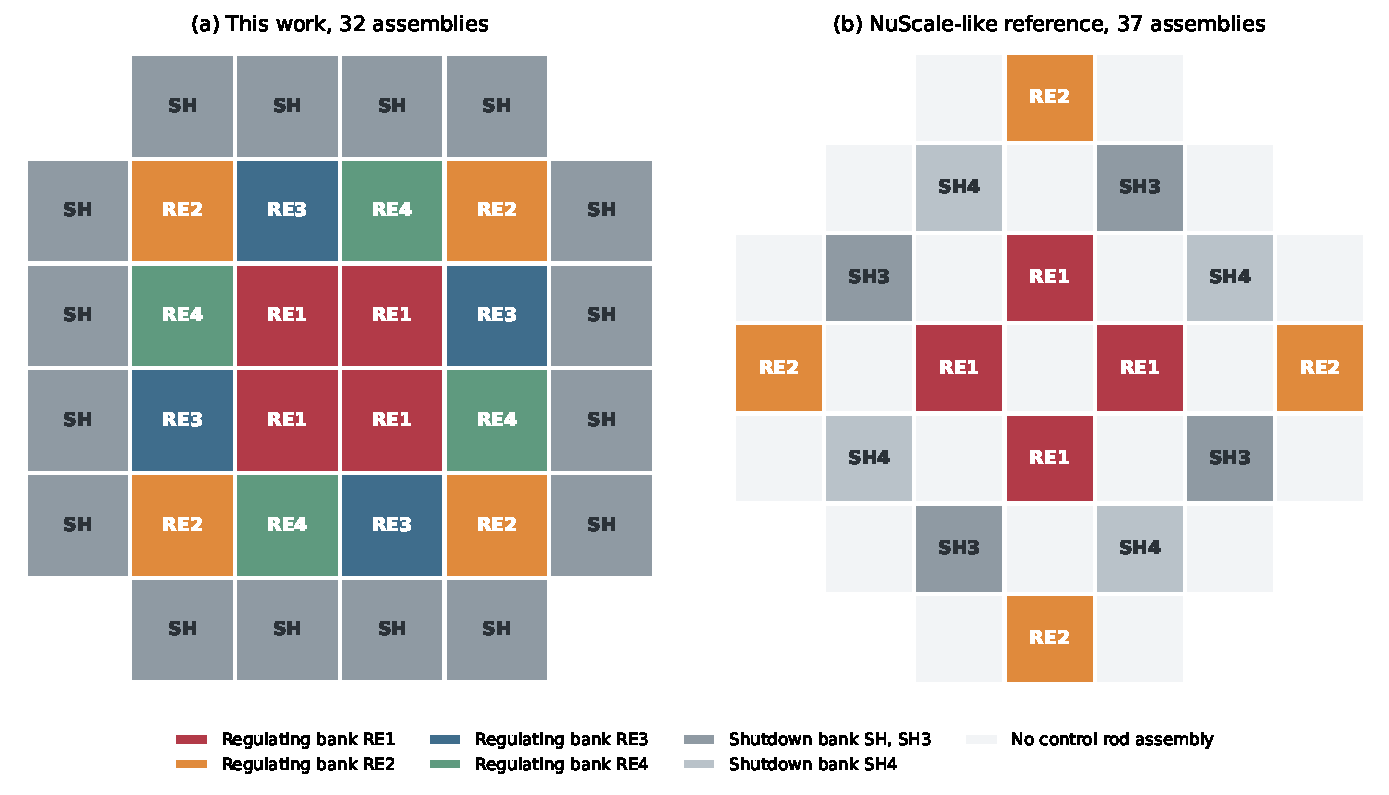
\includegraphics[width=0.85\textwidth]{images/c8_banks_vs_reference}
  \caption[Campaign 8 core and reference specification: control rod banks]{Campaign 8 core and reference specification: control rod banks. (a)~This work. (b)~NuScale-like reference specification.\newline Panel (b) adapted from~\cite{fridman_nuscale_benchmark_2023}.}
  \label{fig:c8-banks-vs-ref}
\end{figure}

The multiplication factor with only banks RE1 and RE2 inserted,
$k_\mathrm{RE12}$, is stored without constraint. Because a core with
the regulating system of the reference specification would have only
these two banks available, $k_\mathrm{RE12} \le 0.99$ is the more
realistic measure of controllability. On the two-dimensional values computed in the campaign, 4 feasible designs satisfy it, C8-53, C8-13, C8-31 and
C8-12. Their unrodded multiplication factors, 1.026 to 1.042, are inside the
two-bank window of Table~\ref{tab:c8-worth}, their beginning-of-life
excess reactivity of \num{2564} to \SI{4068}{pcm} is small, so their
cycles are short, 598 to \SI{3381}{EFPD}, and none of them is on the
front. Design C8-12 is not a candidate, because its cycle length of
\SI{598}{EFPD} is the shortest of the 4 and less than a third of the
minimum cycle length of \SI{1826}{EFPD}, and it was not confirmed in three dimensions.

The two-dimensional reading is conservative
(Section~\ref{sec:res-kt-burnup}).
Table~\ref{tab:c8-twobank} gives the two-bank margin
$M_8 = -\rho(k_\mathrm{RE12})$, positive when subcritical, of the 11
designs re-solved on the three-dimensional core model at
\SI{1000}{ppm} with 2 seeds, in both models at beginning of life and, in three dimensions, at
the operating maximum, where the gadolinium hump of
Section~\ref{sec:res-c8-boron} is subtracted, together with the peaking
factor of the same solves.

\begin{table}[htbp]
  \centering
  \footnotesize
  \begin{threeparttable}
  \caption{Campaign 8 designs: two-bank margin and peaking factor in two and in three dimensions.}
  \label{tab:c8-twobank}
  \setlength{\tabcolsep}{3pt}\scriptsize
  \begin{tabular}{@{}l r r r r r r r c c c@{}}
    \toprule
    Design & $e$ & EFPD & $M_8^\mathrm{2D}$ & $M_8^\mathrm{3D}$ & $M_8^\mathrm{3D,max}$\tnote{a} &
      $F_{\Delta H}^\mathrm{2D}$ & $F_{\Delta H}^\mathrm{3D}$ &
      \multicolumn{3}{c}{Two-bank controllable} \\
    \cmidrule(l){9-11}
    {[--]} & [wt\%] & [d] & [pcm] & [pcm] & [pcm] & [--] & [--] & 2D & 3D & 3D, max \\
    \midrule
    C8-53 & 3.45  & 1142 & 5882   & 8553   & 8553   & 1.494 & 1.475 & yes & yes & yes \\
    C8-47 & 4.39  & 1941 & $-1091$ & 1330  & 1330   & 1.531 & 1.503 & --  & yes & yes \\
    C8-42 & 4.44  & 1968 & $-1315$ & 1052  & 1052   & 1.532 & 1.515 & --  & yes & yes \\
    C8-23 & 4.94  & 2346 & $-4046$ & $-1718$ & $-1718$ & 1.525 & 1.522 & -- & -- & -- \\
    C8-13 & 5.14  & 2383 & 3562   & 5946   & 5946   & 1.603 & 1.573 & yes & yes & yes \\
    C8-29 & 5.90  & 3070 & $-6615$ & $-4412$ & $-7466$ & 1.527 & 1.491 & -- & -- & -- \\
    C8-31 & 6.59  & 3381 & 3491   & 5856   & 901    & 1.627 & 1.596 & yes & yes & --  \\
    C8-21 & 7.81  & 4221 & $-4776$ & $-2598$ & $-3997$ & 1.585 & 1.576 & -- & -- & -- \\
    C8-44 & 9.23  & 5019 & $-5637$ & $-3508$ & $-5465$ & 1.630 & 1.600 & -- & -- & -- \\
    C8-59 & 9.34  & 5104 & $-4691$ & $-2479$ & $-3721$ & 1.625 & 1.603 & -- & -- & -- \\
    C8-1  & 11.03 & 5782 & $-5761$ & $-3700$ & $-3700$ & 1.673 & 1.642 & -- & -- & -- \\
    \bottomrule
  \end{tabular}
  \begin{tablenotes}[flushleft]\footnotesize
    \item[a] Beginning-of-life margin minus the core hump of
      Table~\ref{tab:c8-post-boron} where the hump is positive.
  \end{tablenotes}
  \end{threeparttable}
\end{table}

Figure~\ref{fig:c8-twobank-2d3d} places the designs in the objective
plane, with 5 years at full power drawn as a vertical line, and
compares the two-bank margin of the 11 designs in the two models.
The table and the figure support three results:

\begin{itemize}
  \item \textbf{Movement of the two-bank front:} in two dimensions the
        two-bank designs form the front C8-53, C8-13 and C8-31, none of
        which is on the four-bank front, and only C8-13 and C8-31
        satisfy the refuelling interval. In three dimensions C8-47 and
        C8-42 cross the constraint, by 320 and \SI{42}{pcm} at beginning
        of life, and C8-31 loses it at the operating maximum, where its
        hump of \SI{4955}{pcm} leaves \SI{901}{pcm}. The two-bank front
        becomes C8-47, C8-42 and C8-13. Its short-cycle end coincides
        with that of the four-bank front, so the design with the lowest
        peaking factor of the campaign, C8-47, is controllable with two
        banks.

  \item \textbf{Correction of the two-dimensional reading:} the offset
        between the models is regular. A linear fit over the 11
        designs, $M_8^\mathrm{3D} - M_8^\mathrm{2D} = 0.033\,M_8^\mathrm{2D}
        + \SI{2365}{pcm}$, reproduces them within an rms of
        \SI{83}{pcm}, so a design is two-bank controllable in three
        dimensions when its two-dimensional margin exceeds about
        \SI{-1300}{pcm}. Over the 19 feasible designs of the campaign the corrected reading admits one further design, C8-22, at
        \SI{3684}{EFPD} and $F_{\Delta H} = 1.648$ with
        $M_8^\mathrm{2D} = \SI{+273}{pcm}$, which was not confirmed in
        three dimensions. C8-42, at \SI{-1315}{pcm}, is within the rms
        of the threshold, and only its three-dimensional solve decides
        it.

  \item \textbf{Peaking factor:} the three-dimensional value is lower
        than the two-dimensional one of the same solves by 0.003 to
        0.036. The two-dimensional values, solved at $150\,000$
        particles, are themselves below the campaign values, solved at the campaign setting, by 0.03 for C8-53. That is the fidelity bias of
        a maximum taken over noisy tallies, which
        Section~\ref{sec:res-c9-peaking} measures on the Campaign 9
        front.
\end{itemize}

\begin{figure}[htbp]
  \centering
  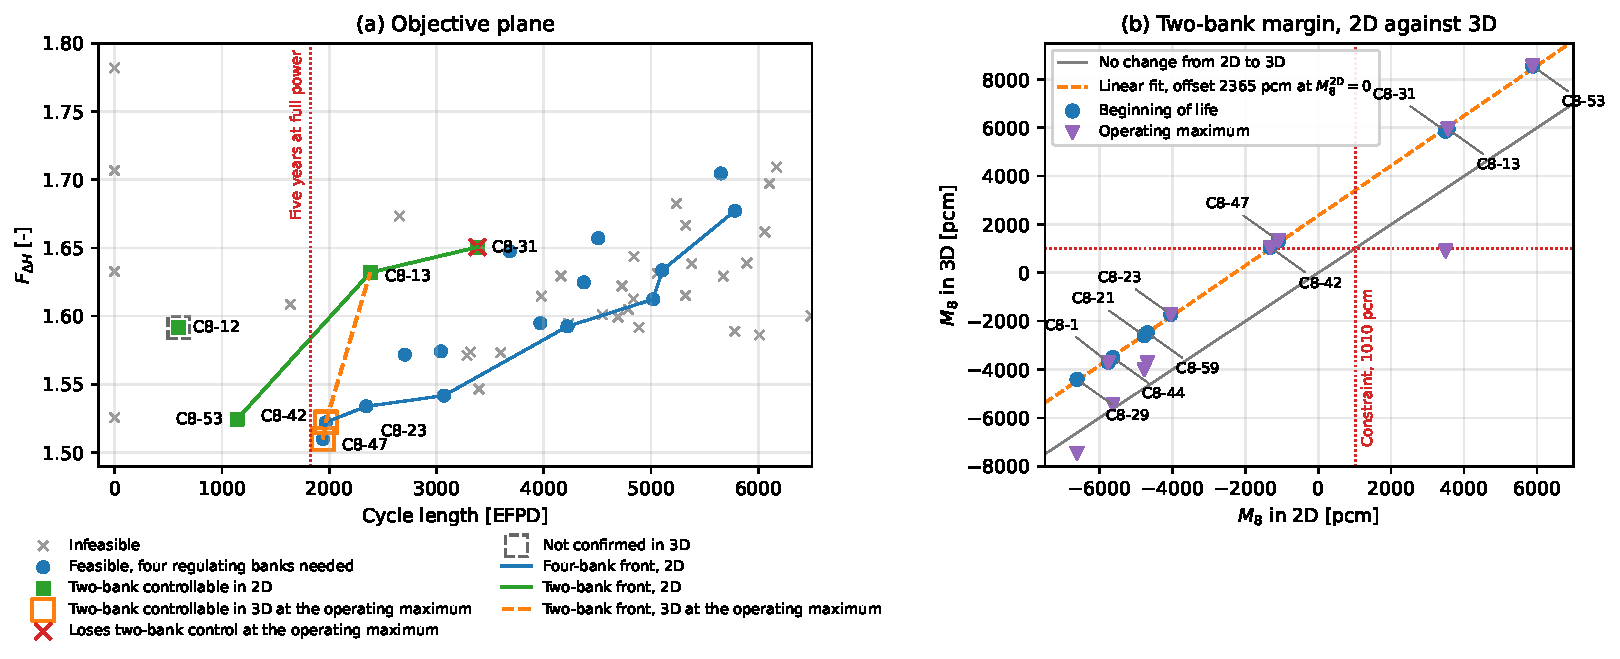
\includegraphics[width=\textwidth]{images/c8_twobank_2d3d}
  \caption{Campaign 8: two-bank designs in two and three dimensions. (a)~Objective plane with the four-bank and the two-bank fronts. (b)~Two-bank margin in three against two dimensions.}
  \label{fig:c8-twobank-2d3d}
\end{figure}

In the two-bank designs the operating physics of a pressurised water
reactor is recognisable. A commercial core at hot full power
compensates its beginning-of-life excess reactivity with soluble boron
and burnable absorber and keeps the regulating banks nearly withdrawn,
so that the rods compensate only the power defect and the reactivity
changes of load following. Table~\ref{tab:c8-front-two} compares the
front with the two-bank designs, with the excess reactivity at
beginning of life $\rho_\mathrm{BOL}$, the reactivity of the unrodded
core at \SI{1000}{ppm}, in pcm. The front designs would need the four
regulating banks at an insertion depth that compensates their excess
reactivity at power with \SI{1000}{ppm} in the coolant, outside
standard PWR operating practice and with the rodded peaking of
Figure~\ref{fig:c8-split} imposed continuously, whereas the excess
reactivity of the two-bank designs is of the order that boron
adjustment alone can compensate.

\begin{table}[htbp]
  \centering
    \small
  \caption{Campaign 8: front against the two-bank designs in each reading.}
  \label{tab:c8-front-two}
  \setlength{\tabcolsep}{5pt}
  \begin{tabular}{@{}lccc@{}}
    \toprule
    Quantity & Front & Two-bank, 2D & Two-bank, 3D \\
    \midrule
    Designs & 8 & C8-53, C8-13, C8-31 & C8-47, C8-42, C8-13 \\
    Regulating banks at power & RE1 to RE4 & RE1 and RE2 & RE1 and RE2 \\
    $\rho_\mathrm{BOL}$ [pcm] & \num{8930} to \num{13627} & \num{2564} to \num{4068} & \num{4068} to \num{9154} \\
    $F_{\Delta H}$ [--] & 1.510 to 1.677 & 1.524 to 1.650 & 1.510 to 1.632 \\
    $\mathrm{EFPD}$ at $F_{\Delta H} \approx 1.52$ [d] & 1941 to 1968 & 1142 & 1941 to 1968 \\
    $\mathrm{EFPD}$ at $F_{\Delta H} \approx 1.63$ [d] & 5104 & 3381 & 2383 \\
    \bottomrule
  \end{tabular}
\end{table}

The comparison of the two fronts and the measured rod worths give four
results:

\begin{itemize}
  \item \textbf{Cost of the two-bank requirement in two dimensions:}
        between 34 and 51 per cent of the cycle length at equal
        peaking.
  \item \textbf{Cost of the two-bank requirement in three dimensions:}
        nothing at the low-peaking end, and 53 per cent at $F_{\Delta H} \approx 1.63$,
        where C8-13 gives \SI{2383}{EFPD} against \SI{5104}{EFPD} for
        the front.
  \item \textbf{Rod worth against the benchmark:} across the evaluated
        designs the 16 control rod assemblies of this core are worth
        \num{11626} to \SI{19294}{pcm}, the same range as the 16 of the
        NuScale-like benchmark, \SI{19231}{pcm}, because the absorber
        densities, the clad radii and the guide-tube geometry are those
        of the benchmark. On the 11 confirmed designs the four regulating
        banks are worth \num{12775} to \SI{18401}{pcm} and the first two
        \num{5830} to \SI{8384}{pcm}.
  \item \textbf{Excess reactivity against the benchmark:} the benchmark
        reports an all-rods-out effective multiplication factor of
        $1.02768 \pm 0.00001$ at beginning of life with \SI{1000}{ppm}
        of soluble boron~\cite{fridman_nuscale_benchmark_2023}, so its
        rods compensate only about \SI{2700}{pcm} of excess reactivity,
        14 per cent of their worth. The two-bank designs of
        Table~\ref{tab:c8-front-two} are in that regime, while the
        excess reactivity of the front is 3 to 5 times that of the
        benchmark.
\end{itemize}

The unrodded $k_\mathrm{eff}^\mathrm{core}$ of every design already
includes the soluble boron at \SI{1000}{ppm} and the gadolinia, so the
excess reactivity that increases the cycle length is the same that the
regulating banks must compensate when inserted.

\subsection{Leakage factors of \texorpdfstring{$k_\mathrm{target}$}{k-target}}
\label{sec:res-kt-burnup}

The leakage-corrected $k_\mathrm{target}$ of Equation~\eqref{eq:ktarget-3d}
is the product of two factors calibrated once at beginning of life, the
radial factor LF of Section~\ref{sec:meth-ktarget}, tabulated on the
reference fuel loading of 4.05 and \SI{4.55}{wt\%} without gadolinia,
and the axial factor $L_\mathrm{ax} = 1.0289$ of
Section~\ref{sec:res-c6-lax}.

Every cycle length of the Campaign 8 front, 1941 to \SI{5782}{EFPD}, is
computed against that $k_\mathrm{target}$ on designs whose ring
enrichments of 3.16 to \SI{12.68}{wt\%} and gadolinia loadings of 0.18
to \SI{7.43}{wt\%} are far from the reference assembly. This section
therefore measures the dependence of each factor on the variables that
the campaign moves or the model fixes, and Table~\ref{tab:kt-relations}
collects the relations for a later campaign.

The burnup dependence of the radial factor was measured on the 8 front
members and on the two-bank designs C8-31 and C8-53, the second of
which extends the enrichment range of the test to \SI{3.45}{wt\%}. At
beginning of life and at the depletion steps before and after the end
of cycle, the nuclide inventory of the assembly depletion of each design
was loaded into the reflective assembly and into all 32 assemblies of
the core, and each was solved as a criticality calculation with 3
seeds. Table~\ref{tab:kt-burnup} gives for each design the drift, the
change of the factor between beginning and end of cycle, the residual
$r_\mathrm{BOL}$, the factor at beginning of life minus the tabulated
$k_\mathrm{target}$, and the correction $\Delta\mathrm{EFPD}$ of the
reported cycle length that the end-of-cycle factor implies, positive
when the reported cycle is too short. The factor is constant over the
cycle if the drifts pass two tests:

\begin{itemize}
  \item \textbf{Common drift:} their $\chi^2$~\cite{david_nagaraja_2003}
        about the inverse-variance weighted
        mean~\cite{lux_koblinger_1991} is within the range expected from
        their errors.
  \item \textbf{Zero drift:} the weighted mean is within its own error of
        zero.
\end{itemize}

\begin{table}[htbp]
  \centering
  \small
  \caption{Campaign 8 designs: burnup dependence of the leakage factor of $k_\mathrm{target}$.}
  \label{tab:kt-burnup}
  \begin{tabular}{@{}ccccccc@{}}
    \toprule
    Design & $e$ & $B_\mathrm{EOC}$ & $k_\mathrm{target}$ &
      $r_\mathrm{BOL}$ & Drift & $\Delta\mathrm{EFPD}$ \\
    {[--]} & [wt\%] & [MWd/kgHM] & [--] & [pcm] & [pcm] & [d] \\
    \midrule
    C8-1  & 11.03 & 57.8 & 1.0829 & $-329$ & $+33 \pm 126$  & $+56$ \\
    C8-59 & 9.34  & 50.2 & 1.0820 & $-220$ & $-4 \pm 107$   & $+43$ \\
    C8-44 & 9.23  & 49.8 & 1.0822 & $-219$ & $-10 \pm 90$   & $+42$ \\
    C8-21 & 7.81  & 42.3 & 1.0824 & $-222$ & $+149 \pm 84$  & $+11$ \\
    C8-31 & 6.59  & 33.4 & 1.0828 & $-85$  & $-10 \pm 85$   & $+14$ \\
    C8-29 & 5.90  & 31.0 & 1.0825 & $-9$   & $-152 \pm 99$  & $+25$ \\
    C8-23 & 4.94  & 23.7 & 1.0824 & $+53$  & $-67 \pm 116$  & $+2$ \\
    C8-42 & 4.44  & 19.7 & 1.0830 & $+54$  & $-22 \pm 82$   & $-4$ \\
    C8-47 & 4.39  & 19.5 & 1.0827 & $+27$  & $+2 \pm 107$   & $-4$ \\
    C8-53 & 3.45  & 10.8 & 1.0825 & $+174$ & $-84 \pm 88$   & $-14$ \\
    \bottomrule
  \end{tabular}
\end{table}

Three further measurements complete the test. The enrichment
dependence was measured on the fresh reference assembly without
gadolinia and on its two-dimensional core, for 6 enrichments from 3 to
\SI{13}{wt\%} and 7 reflector thicknesses from 2.0 to \SI{5.66}{cm}, 42
core solves with one seed. The axial factor was measured on the
three-dimensional core model of the 11 confirmed designs at
\SI{1000}{ppm} in the 3 rod configurations with 2 seeds, whose
two-dimensional solves reproduce the campaign values within $-53$ to
\SI{+69}{pcm}. The downcomer sensitivity was measured on C8-47, C8-21
and C8-59 with the reflector thinned to \SI{3.969}{cm}, a downcomer of
\SI{3.7}{cm} instead of the minimum of \SI{2.0}{cm}. The measurements
give four results:

\begin{itemize}
  \item \textbf{Burnup:} the 10 drifts share one weighted mean, with
        $\chi^2 = 6.73$ on 9 degrees of freedom, $p = 0.66$, and that
        mean is within its error of zero, so the radial factor is
        constant over the cycle within \SI{60}{pcm}, 7 to \SI{11}{d} of
        cycle length, and the burnup assumption is valid.
  \item \textbf{Enrichment:} the beginning-of-life residual is ordered
        by the enrichment, $r_\mathrm{BOL} = 341 - 62.5\,e$ in pcm with a
        Pearson coefficient of $-0.975$, and the reference assembly
        without gadolinia gives the same slope, so the effect comes from
        the enrichment and not from the gadolinia. Because
        $k_\mathrm{target}$ was computed once on the reference assembly,
        it is too high for a design of higher enrichment, so the long
        cycles are conservative (Table~\ref{tab:kt-burnup}), the
        ordering of Table~\ref{tab:c8-front} is unchanged, and at the
        upper enrichment bound of \SI{13.9}{wt\%} the error is about 500
        to \SI{600}{pcm}. The reflector thickness has a smaller effect.
  \item \textbf{Rod configuration:} the unrodded axial factor agrees
        with the Campaign 6 study and is higher at low enrichment, partly
        because of the withdrawn rods of the model, so the campaign value
        of 1.0289 is correct for the long-cycle designs and low for the
        low-peaking end of the front. With rods inserted the factor
        decreases, because the rod of the reference specification absorbs
        less in three dimensions than the full-height B$_4$C of the
        two-dimensional constraint (Section~\ref{sec:meth-ctrl}). The
        axial leakage still leaves the rodded three-dimensional core less
        reactive than the two-dimensional one, so the two-dimensional
        constraint admits no design that the three-dimensional core
        would reject, and Section~\ref{sec:res-c8-split} applies the
        two-bank offset as the correction of the two-dimensional reading.
  \item \textbf{Downcomer:} the wider downcomer changes the peaking
        factor by at most one seed standard deviation, so a downcomer of
        \SI{3.7}{cm} can be adopted for every candidate at a cost of at
        most \SI{60}{pcm} at beginning of life.
\end{itemize}

The enrichment dependence of the radial factor is the one relation
large enough to change whether a design is accepted, and
Section~\ref{sec:concl-limits} lists it among the limitations, with an
enrichment-dependent $k_\mathrm{target}$ among the continuations of
Section~\ref{sec:concl-future}.

\begin{table}[htbp]
  \centering
  \footnotesize
  \caption{Campaign 8: measured dependence of the leakage factors of $k_\mathrm{target}$.}
  \label{tab:kt-relations}
  \begin{tabularx}{\textwidth}{@{}>{\raggedright\arraybackslash}p{3.4cm}c>{\raggedright\arraybackslash}X>{\raggedright\arraybackslash}p{3.0cm}@{}}
    \toprule
    Variable & Factor & Effect & Basis \\
    \midrule
    Burnup, beginning to end of cycle & LF & $-13 \pm \SI{30}{pcm}$, constant & 10 designs, 3 seeds \\
    Enrichment & LF & $-64 \pm \SI{9}{pcm}$ per wt\%, from $-104$ at \SI{4}{wt\%} to $-34$ at \SI{11}{wt\%} & 42 grid points, 1 seed \\
    Reflector thickness, 2.0 to \SI{5.66}{cm} & LF & 60 to \SI{135}{pcm} at fixed pitch & 42 grid points, 1 seed \\
    Pitch, 1.15 to \SI{1.43}{cm} & $k_\mathrm{target}$ & about \SI{-2100}{pcm} & Campaign 2 to 7 grid \\
    Rod configuration & $L_\mathrm{ax}$ & 1.0286 to 1.0311 unrodded, 1.0219 to 1.0252 with two banks, 1.0126 to 1.0177 with four & 11 designs, 2 seeds \\
    Rod insertion & 2D controllability constraint & conservative by 2062 to \SI{2671}{pcm} with two banks, 1272 to \SI{2047}{pcm} with four & 11 designs, 2 seeds \\
    Withdrawn rods in the model & $L_\mathrm{ax}$ & \SI{+129}{pcm} & C8-47 \\
    Enrichment & $L_\mathrm{ax}$ & 120 to \SI{220}{pcm} higher below \SI{5.9}{wt\%} & 11 designs, 2 seeds \\
    Downcomer, 2.0 to \SI{3.7}{cm} & $k_\mathrm{2D}$ & $-17$ to \SI{-59}{pcm} & 3 designs, 2 seeds \\
    \bottomrule
  \end{tabularx}
\end{table}

%% labels of the material summarised above, kept so that the
%% cross-references of the other chapters still resolve
\label{sec:res-c8-refl}\label{fig:c8-post-refl}\label{tab:kt-enrich}\label{tab:c8-3d-lax}\label{tab:c8-3d-downcomer}

\subsection{Candidate decision}
\label{sec:res-c8-decision}

Table~\ref{tab:c8-candidates} gives the 8 front members and the
2 two-bank designs that satisfy the refuelling interval, with the quantities that determine the decision.

\begin{table}[!htb]
  \centering
  \footnotesize
  \begin{threeparttable}
  \caption{Campaign 8: candidate designs.}
  \label{tab:c8-candidates}
  \setlength{\tabcolsep}{2.6pt}\scriptsize
  \begin{tabular}{@{}llrrrrrrrrr@{}}
    \toprule
    Design & Role & EFPD & $e$ & $w_\mathrm{Gd}$ & $n_\mathrm{Gd}$ &
      $t_\mathrm{refl}$ & $F_{\Delta H}$ & $F_{\Delta H}^\mathrm{3D}$ &
      $c_\mathrm{peak}$ & $M_8^\mathrm{3D,max}$ \\
    {[--]} & {[--]} & [d] & [wt\%] & [wt\%] & [rods] & [cm] & [--] & [--] &
      [ppm] & [pcm] \\
    \midrule
    \textbf{C8-47} & \textbf{Recommended} & 1941 & 4.39 & 2.88 & 12 & 4.29 & 1.510 & 1.503 & 2348 & 1330 \\
    C8-42 & Front member & 1968 & 4.44 & 2.88 & 12 & 3.76 & 1.522 & 1.515 & 2377 & 1052 \\
    C8-23 & Front member & 2346 & 4.94 & 2.80 & 12 & 4.81 & 1.534 & 1.522 & 2979 & $-1718$ \\
    C8-29 & Front member & 3070 & 5.90 & 0.18 & 40 & 4.69 & 1.542 & 1.491 & 4277 & $-7466$ \\
    C8-21 & Front member & 4221 & 7.81 & 3.11 & 32 & 4.92 & 1.592 & 1.576 & 4095 & $-3997$ \\
    C8-44 & Front member & 5019 & 9.23 & 3.20 & 40 & 5.33 & 1.612 & 1.600 & 4940 & $-5465$ \\
    C8-59 & Front member & 5104 & 9.34 & 4.32 & 40 & 5.66 & 1.634 & 1.603 & 4473 & $-3721$ \\
    C8-1 & Front member & 5782 & 11.03 & 7.43 & 40 & 3.94 & 1.677 & 1.642 & 4674 & $-3700$ \\
    C8-13 & Two-bank alternative & 2383 & 5.14 & 5.25 & 24 & 3.15 & 1.632 & 1.573 & 1697 & 5946 \\
    C8-31 & Two-bank at BOL only\tnote{a} & 3381 & 6.59 & 3.38 & 40 & 4.18 & 1.650 & 1.596 & 2760 & 901 \\
    \bottomrule
  \end{tabular}
  \begin{tablenotes}[flushleft]\footnotesize
        \item[a] Two-bank controllable at beginning of life only,
      \SI{901}{pcm} at the operating maximum.
    \item $F_{\Delta H}^\mathrm{3D}$ and $M_8^\mathrm{3D,max}$ from
      Table~\ref{tab:c8-twobank}, $c_\mathrm{peak}$ from
      Table~\ref{tab:c8-post-boron}.
  \end{tablenotes}
  \end{threeparttable}
\end{table}

Design C8-47 is the recommended design, because it satisfies
both criteria of the post-analysis:

\begin{itemize}
  \item \textbf{Radial peaking:} it is the minimum-peaking member of the
        feasible front, at \SI{1941}{EFPD}, $F_{\Delta H} = 1.510$ and
        \SI{4.39}{wt\%} assembly enrichment.

  \item \textbf{Two-bank control:} it is controllable with the first two
        regulating banks at \SI{1000}{ppm} on the three-dimensional
        core, with a margin of \SI{1330}{pcm} that survives the
        gadolinium hump because its beginning of life is its most
        reactive state (Table~\ref{tab:c8-post-boron}).
\end{itemize}

Its cycle length is the shortest on the front and is above the minimum
cycle length of \SI{1826}{EFPD} by
\SI{115}{EFPD}. Because both criteria reward a small beginning-of-life
excess, and the low-enrichment end of the front has the smallest excess
that still satisfies the minimum cycle length, the same design leads both.

Table~\ref{tab:c8-candidates} leaves one alternative with a longer
cycle length under two-bank control, and excludes the others:

\begin{itemize}
  \item \textbf{C8-13, the two-bank alternative:} it is above the
minimum cycle length by \SI{557}{EFPD}, has the largest two-bank
        margin of the table at the operating maximum, \SI{5946}{pcm} in
        three dimensions, and needs the least boron of any design that
        satisfies the minimum cycle length, \SI{1697}{ppm}. Its cost is the peaking
        factor, 1.632 against 1.510.

  \item \textbf{C8-42:} its cycle length, peaking factor and two-bank
        margin differ from those of C8-47 by \SI{27}{EFPD}, 0.012 and
        \SI{278}{pcm}, none of them statistically significant, so it is
        the same choice and not a second alternative.

  \item \textbf{The long-cycle front members:} C8-29 to C8-1 need 4095
        to \SI{4940}{ppm} at the operating maximum, above the MTC boron
        limit of 2758 to \SI{3008}{ppm} measured on the lattice of
        C8-47, and their two-bank margin is negative. Their cycle length
        can only be compensated with the four regulating banks at a
        large insertion depth, so a longer cycle is not available under
        boron control. C8-23, at \SI{2979}{ppm}, is below the limit at
        \SI{15.5}{MPa} only.

  \item \textbf{C8-31:} it is controllable with two banks at beginning
        of life, but its gadolinium hump leaves \SI{901}{pcm} at the
        operating maximum, below the constraint, and its
        \SI{2760}{ppm} is at the MTC boron limit at \SI{12.8}{MPa}.
\end{itemize}

\section{Campaign 9: minimum critical boron concentration \texorpdfstring{$c_\mathrm{max}$}{c max} and minimum radial peaking factor \texorpdfstring{$F_{\Delta H}$}{F dH}}
\sectionmark{Campaign 9: boron and peaking}
\label{sec:res-c9}\label{sec:res-c8-retro}

Campaign 8 closed with three findings that motivate the reformulation:

\begin{itemize}
  \item \textbf{The cycle length was not the binding requirement:}
        every front design satisfies the refuelling interval of
        \SI{1826}{EFPD} (Section~\ref{sec:res-c8-mission}).

  \item \textbf{Controllability decided the feasible region:} the
        longer cycles require a beginning-of-life excess reactivity of
        \num{8930} to \SI{13627}{pcm}, which only the four regulating
        banks at a large insertion depth can compensate, and the
        controllability constraint rejected 35 of the 41 infeasible
        designs (Section~\ref{sec:res-c8-screens}).

  \item \textbf{Boron divides the front at the same place:} the
        long-cycle members need 3677 to \SI{4674}{ppm}, above the MTC
        boron limit, whereas the short-cycle end and the two-bank designs
        stay below it (Section~\ref{sec:res-c8-mtc}).
\end{itemize}

Because a cycle beyond the required cycle length of \SI{1826}{EFPD} requires excess reactivity that the
rods and the boron must compensate, the reformulated problem of
Section~\ref{sec:meth-c9} applies the cycle length as a constraint at
\SI{1826}{EFPD} and minimises the peaking factor and the critical boron
concentration at the operating maximum, $c_\mathrm{max}$, which
includes the gadolinium hump.

\subsection{Specification}
\label{sec:res-c9-formulation}

The campaign changes the formulation of Section~\ref{sec:meth-c9},
extends the enrichment range down to \SI{2.0}{wt\%} and keeps the rest
of Campaign 8 (Table~\ref{tab:c89-spec}). The
objectives are the radial peaking factor
$F_{\Delta H}$ with all rods out and the critical boron concentration
at the operating maximum $c_\mathrm{max}$ of
Equation~\eqref{eq:c9-cmax}, both minimised, two constraints are new
and the peaking bound is lowered.

\begin{align}
g_\mathrm{efpd}(\mathbf{x}) &= 1826 - \mathrm{EFPD}(\mathbf{x}) \le 0
\label{eq:c9-g-efpd} \\
g_\mathrm{ctrl,peak}(\mathbf{x}) &= k_\mathrm{RE,peak}(\mathbf{x}) - (1 - \Delta\rho_\mathrm{op}) \le 0
\label{eq:c9-g-ctrl-peak} \\
g_\mathrm{peak}(\mathbf{x}) &= F_{\Delta H}(\mathbf{x}) - 1.65 \le 0
\label{eq:c9-g-peak}
\end{align}

\noindent where the symbols have the following meaning.

\begin{itemize}
  \item $g_\mathrm{efpd}$ is the minimum cycle-length constraint, in d,
        with $\mathrm{EFPD}$ the cycle length of the assembly depletion
        of Section~\ref{sec:objective_functions} and 1826 the five-year
        requirement of Section~\ref{sec:meth-c9}.

  \item $g_\mathrm{ctrl,peak}$ is the controllability constraint at the
        operating maximum, dimensionless, with $k_\mathrm{RE,peak}$ the
        multiplication factor of the core with banks RE1 to RE4
        inserted at the most reactive point of the cycle, obtained from
        $k_\mathrm{RE}$ of Equation~\eqref{eq:k-re} by adding the core
        hump $L\,\Delta\rho_\mathrm{hump}$ of
        Equation~\eqref{eq:c9-cmax} to its reactivity where the hump is
        positive, and $\Delta\rho_\mathrm{op}$ the operating margin of
        \SI{1000}{pcm} of Equation~\eqref{eq:g-ctrl-meth}.

  \item $g_\mathrm{peak}$ is the peaking constraint, dimensionless,
        with the bound lowered from the 2.0 of
        Table~\ref{tab:constraints} to 1.65.
\end{itemize}

Beyond the depletion of the reflective assembly, which gives the cycle
length and the hump, each evaluation executes 4 to 6 static
solves:

\begin{itemize}
  \item \textbf{Assembly at beginning of life:} $k_\infty$ of the
        reflective assembly, for the leakage-corrected $k_\mathrm{target}$.
  \item \textbf{Core, all rods out, 1000 ppm:}
        $k_\mathrm{eff}^\mathrm{core}$ for the reactivity window,
        $F_{\Delta H}$ for the objective and the peaking bound,
        and $\rho(1000)$ for the boron objective.
  \item \textbf{Core with RE1 to RE4 inserted:} $k_\mathrm{RE}$
        for $g_\mathrm{ctrl}$ of Equation~\eqref{eq:g-ctrl-meth}, and,
        with the core hump added to its reactivity, $k_\mathrm{RE,peak}$
        for $g_\mathrm{ctrl,peak}$ of Equation~\eqref{eq:c9-g-ctrl-peak}.
  \item \textbf{Core with RE1 and RE2 inserted:} $k_\mathrm{RE12}$,
        the two-bank reading, stored and not constrained.
  \item \textbf{Core, all rods out, at one or 2 further
        concentrations:} the boron measurement of
        Section~\ref{sec:meth-c9}. If $\rho(1000) > 0$ the core is
        solved again at \SI{2000}{ppm}, and if $\rho(1000) \le 0$ at
        \SI{0}{ppm}. If no 2 measured points are yet on either side
        of the sign change, one more solve is made at \SI{3000}{ppm}.

\end{itemize}

The cost of the campaign on the reference workstation divides into
three parts.

\begin{itemize}
  \item \textbf{Total:} 60 evaluations in \SI{18.65}{h}, \SI{2.37}{h}
        less than Campaign 8.
  \item \textbf{Depletion at assembly level:} \SI{10.47}{h}, \SI{56}{\%}
        of the campaign, against \SI{15.42}{h} in Campaign 8, at 10.5
        depletion steps per design against 14.6. Because the
        minimisation of $c_\mathrm{max}$ directs the infill batches
        towards designs of small excess reactivity, the infill designs
        have a mean cycle length of \SI{1742}{EFPD} and 7.9 steps,
        against \SI{3338}{EFPD} and 12.2 steps in the design of
        experiments.
  \item \textbf{Core solves of the constraints and of the reference
        concentration:} 3 per design, \SI{5.28}{h} together.
    \item \textbf{Boron measurement:} \SI{2.71}{h}, \SI{14.5}{\%}, at one
        or 2 extra core solves per design, 30 designs with 1 and 30
        with 2, the second wherever a root exceeds \SI{2000}{ppm}, 90
        boron solves for 60 designs, against the \SI{3}{\%} increment
        that moved the peaking objective to core level in Campaign 4.
\end{itemize}

\subsection{Search}
\label{sec:res-c9-search}\label{sec:res-c9-convergence}
\label{fig:c9-hv}\label{fig:c9-learning}\label{fig:c9-front-stability}

The search executed a design of experiments of 24 evaluations and 6
infill iterations of 6 evaluations each, and Table~\ref{tab:c9-hv} gives
the hypervolume of the feasible non-dominated designs after the design
of experiments and after each iteration. The hypervolume did not change over the last 3 values, 2 iterations
without gain against the 3 that the stopping rule of
Section~\ref{sec:meth-loop-stop} requires, and the campaign was stopped
there because the evaluated designs were already concentrated, with no
change in the membership of the front over the last 12 evaluations.

\begin{table}[htbp]
  \centering
  \small
  \caption{Campaign 9: hypervolume by infill iteration.}
  \label{tab:c9-hv}
  \begin{tabular}{@{}lrrr@{}}
    \toprule
    Stage & Evaluations & Hypervolume & Gain [\%] \\
    \midrule
    Design of experiments & 1 to 24 & 879.1 & -- \\
    Iteration 1 & 25 to 30 & 1244.5 & 41.6 \\
    Iteration 2 & 31 to 36 & 1291.4 & 3.8 \\
    Iteration 3 & 37 to 42 & 1291.6 & 0.02 \\
    Iteration 4 & 43 to 48 & 1318.5 & 2.1 \\
    Iteration 5 & 49 to 54 & 1318.5 & 0.00 \\
    Iteration 6 & 55 to 60 & 1318.5 & 0.00 \\
    \bottomrule
  \end{tabular}
\end{table}

Figure~\ref{fig:c9-evolution} shows the two objectives of every
evaluated design along the evaluation order, by block. The design of
experiments spans the full range of both objectives, with 8 designs
at the \SI{6000}{ppm} truncation, and its 5 feasible designs need
1979 to \SI{4371}{ppm}. From the first infill iteration no design
exceeds 1.62 in $F_{\Delta H}$ or \SI{3300}{ppm} in $c_\mathrm{max}$,
and the 5 front members are found in the second, third and fourth
iterations.

\begin{figure}[!htb]
  \centering
  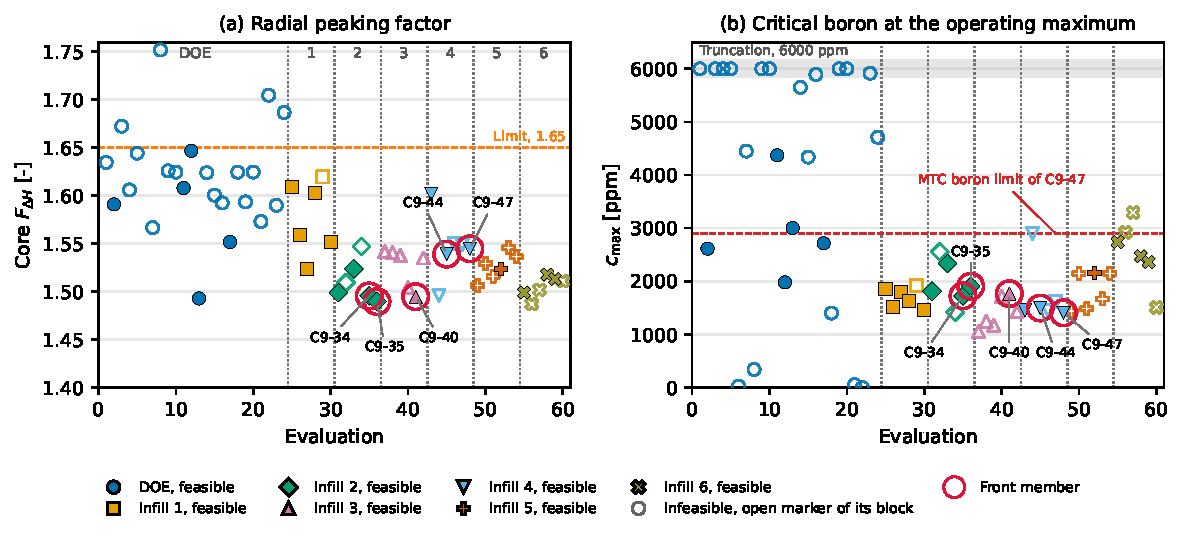
\includegraphics[width=0.95\textwidth]{images/c9_objectives_evolution}
  \caption{Campaign 9: objectives along the evaluation order.}
  \label{fig:c9-evolution}
\end{figure}

\subsubsection{Acquisition health}
\label{sec:res-c9-acq}

The campaign was stopped one iteration short of the stopping rule
because the evaluated designs were concentrated, and
Table~\ref{tab:c9-acq-health} gives the two indicators that determined that decision:

\begin{itemize}
  \item \textbf{Relaxations of the batch-diversity threshold:} the
        number of halvings of $\delta_\mathrm{min}$ of
        Equation~\eqref{eq:batch-div}. The count increased over the
        first iterations and remained constant from the third, so the
        surrogate front no longer contained designs far enough from the
        evaluated ones to fill a batch at the required separation, and
        the search had concentrated on the region already sampled.
  \item \textbf{Margin-feasible candidates:} those with a margin score
        $s_i \le 0$ in Equation~\eqref{eq:feas-margin}, 0 of 300 in every
        iteration, against 25 to 59 of 300 in Campaign 8.
\end{itemize}

\begin{table}[htbp]
  \centering
  \caption{Campaign 9: acquisition health indicators and outcome by infill batch.}
  \label{tab:c9-acq-health}
  \small
  \begin{tabular}{@{}clcccc@{}}
    \toprule
    Iteration & Designs & Margin-feasible & Relaxations & Feasible & Below \SI{1826}{EFPD} \\
    \midrule
    1 & C9-24 to C9-29 & 0/300 & 1 & 5/6 & 1 \\
    2 & C9-30 to C9-35 & 0/300 & 2 & 4/6 & 2 \\
    3 & C9-36 to C9-41 & 0/300 & 3 & 1/6 & 4 \\
    4 & C9-42 to C9-47 & 0/300 & 3 & 3/6 & 3 \\
    5 & C9-48 to C9-53 & 0/300 & 3 & 1/6 & 5 \\
    6 & C9-54 to C9-59 & 0/300 & 3 & 3/6 & 2 \\
    \midrule
    Total &            &       &   & 17/36 & 17 \\
    \bottomrule
  \end{tabular}
\end{table}

The margin was inactive for the first time in the study, against 160
to 266 of 300 margin-feasible candidates per iteration in Campaign 6 and
25 to 59 in Campaign 8, because of the new objective. Minimising
$c_\mathrm{max}$ minimises the excess reactivity and with it the cycle
length, so the front is on the active constraint $g_\mathrm{efpd}$ of
Equation~\eqref{eq:c9-g-efpd}, at \SI{1826}{EFPD}. With the parameters of the acquisition function, $s_i \le 0$ and
$\kappa = 1.5$ of the acquisition step, the
exploration step of the loop, a candidate is margin-feasible only with
a predicted cycle about \SI{42}{d} longer than the minimum of
$g_\mathrm{efpd}$, which requires more excess
reactivity and more boron, so NSGA-II places it in a later
non-dominated front and not in the rank-1 set from which the batch is
selected. Every batch therefore came from the fallback ordering of
Section~\ref{sec:meth-acq}, ascending $s_i$, which selects by confidence in the predicted cycle
length and not by the exploration score $a_i$, and 17 of the 36
infill designs were evaluated below the minimum of
$g_\mathrm{efpd}$.

Whether the inactive margin determined where the batches were placed and
how concentrated they were was tested by
re-executing the acquisition a posteriori, on the 60 stored evaluations
of the campaign and without transport evaluations. The re-execution
compares 6 configurations of the batch selection of the acquisition
function of Section~\ref{sec:meth-acq}, which differ only in how the
candidates are screened and ordered for feasibility:

\begin{itemize}
    \item \textbf{Rule 1, margin with $\kappa = 1.5$, as executed:} the
        configuration of the campaign as it was executed,
        Equation~\eqref{eq:feas-margin} on every surrogate constraint,
        then the fallback ordering, against which rules 2 to 6 are
        compared.
  \item \textbf{Rule 2, margin with $\kappa = 0.5$ on the cycle length:}
        rule 1 with the coefficient reduced on that constraint only,
        $g_\mathrm{efpd}$ of Equation~\eqref{eq:c9-g-efpd}.
  \item \textbf{Rule 3, margin without the cycle length:} rule 1 with
        that constraint, $g_\mathrm{efpd}$ of
        Equation~\eqref{eq:c9-g-efpd}, removed from the margin score.
  \item \textbf{Rule 4, margin, MTC boron limit constrained:} rule 1
        with the limit of \SI{2763}{ppm} added as a surrogate constraint
        on $c_\mathrm{max}$.
  \item \textbf{Rule 5, probability of feasibility, no margin:} the
        candidates ranked by their posterior probability of satisfying
        every surrogate constraint, with no margin score, threshold or
        fallback, so not the campaign rule at $\kappa = 0$.
  \item \textbf{Rule 6, probability of feasibility, MTC boron limit
        constrained:} rule 5 with the same added constraint.
\end{itemize}

For each iteration, the surrogates were refitted on the evaluations
completed before it, 24 for the first up to 54 for the sixth, the same
refits as the walk-forward validation of
Section~\ref{sec:res-c9-validation}, NSGA-II was executed with the
campaign settings and the batch of 6 was selected by each
configuration, and
Table~\ref{tab:c9-acq-replay} gives, over the 36 selections of each
rule, the number below \SI{1}{wt\%} of gadolinia, the region that needs
more boron than the MTC boron limit and contains no feasible design, the
number whose predicted $c_\mathrm{max}$ exceeds the limit, and the
separation of the batches.

The region below \SI{1}{wt\%} is important because at a low gadolinia loading the MTC boron limit is lowest and the
critical boron concentration highest, so the 2 lattices scanned there,
C9-12 and C9-57, exceed their own limit by 912 and \SI{193}{ppm}, which
places the boundary at roughly \SI{1}{wt\%}
(Section~\ref{sec:res-c9-ceiling}), and because Campaign 9 placed 6 of
its 36 infill evaluations there.

\begin{table}[!htb]
  \centering
  \footnotesize
  \caption{Campaign 9: a posteriori acquisition with 6 batch-selection configurations.}
  \label{tab:c9-acq-replay}
    \setlength{\tabcolsep}{4pt}
    \begin{tabularx}{\textwidth}{@{}c>{\raggedright\arraybackslash}Xcccc@{}}
    \toprule
    Rule & Selection rule & Below & Above the & Mean & Minimum \\
     & & \SI{1}{wt\%} Gd & MTC limit & separation & separation \\
    \midrule
        1 & Margin with $\kappa = 1.5$, as executed & 11 & 1 & 0.158 & 0.031 \\
    2 & Margin, $\kappa = 0.5$ on cycle length & 12 & 2 & 0.172 & 0.029 \\
    3 & Margin without the cycle length & 18 & 3 & 0.167 & 0.023 \\
    4 & Margin, MTC-constrained & 5 & 0 & 0.128 & 0.034 \\
    \addlinespace[2pt]
    5 & Feasibility probability, no margin & 17 & 3 & 0.158 & 0.029 \\
    6 & Feasibility probability, MTC-constrained & 8 & 0 & 0.114 & 0.032 \\
    \bottomrule
  \end{tabularx}
\end{table}

The re-execution supports three results:

\begin{itemize}
  \item \textbf{The unconstrained MTC boron limit, not the inactive margin, determined where the batches were placed:} rule 4 against rule 1 reduces
        the selections below \SI{1}{wt\%} from 11 to 5 of 36 and those
        above the limit from 1 to 0, whereas rules 2 and 3, which lower or remove the cycle-length term of the margin, still send 12
        and 18 of 36 selections below \SI{1}{wt\%} and 2 and 3 above
        the limit.
        Every constraint of the specification of
        Section~\ref{sec:res-c9-formulation} is satisfied in that region and the limit is stored but not constrained.
  \item \textbf{A probability-of-feasibility ranking alone is worse:}
        rule 5 sends 17 of 36 selections below \SI{1}{wt\%} and 3 above
        the limit, and rule 6, with the limit constrained, sends 8 below
        \SI{1}{wt\%}, against 5 for rule 4.
  \item \textbf{The spread of a batch is determined by the candidates,
        not by the rule:} rules 1 to 6 give a mean separation of 0.11
        to 0.17 and a minimum of 0.02 to 0.03, below the 0.14 the loop
        requires, because the 300 candidates of the surrogate front are
        themselves concentrated.
\end{itemize}

The acquisition function therefore worked as it was built, and the
placement and concentration of the batches are consequences of how
Campaign 9 was formulated, with the cycle-length constraint active on
the front and the MTC boron limit outside the constraints. A further
campaign should therefore constrain the MTC boron limit inside the loop and use a margin that remains
active at a constraint boundary, which Section~\ref{sec:concl-future}
lists.

\subsection{Feasibility}
\label{sec:res-c9-feasibility}

Of the 60 designs evaluated, 22 satisfy every constraint.
Table~\ref{tab:c9-constraints} gives the number of designs that violate
each constraint, next to the number of Campaign 8
(Table~\ref{tab:c8-violations}), with the limit of each constraint and
the range of its values over the 60 designs.

\begin{table}[htbp]
  \centering
    \caption{Campaigns 8 and 9, 60 evaluations each: designs that violate each constraint.}
  \label{tab:c9-constraints}
  \small
  \setlength{\tabcolsep}{4pt}
  \begin{tabular}{@{}llrrrr@{}}
    \toprule
    Constraint & Limit in Campaign 9 & \multicolumn{2}{c}{Violated by} & \multicolumn{2}{c}{Campaign 9 value} \\
    \cmidrule(lr){3-4}\cmidrule(lr){5-6}
     & & C8 & C9 & Minimum & Maximum \\
    \midrule
    $g_\mathrm{ctrl}$      & $k_\mathrm{RE} \le 0.99$ & 35 & 13 & $-0.326$ & $+0.132$ \\
    $g_{k\max}$            & $k_\mathrm{eff}^\mathrm{core} \le 1.166$ & 23 & 14 & $-0.392$ & $+0.137$ \\
    $g_{k\min}$            & $k_\mathrm{eff}^\mathrm{core} \ge 1.02$ & 6 & 10 & $-0.283$ & $+0.246$ \\
    $g_\mathrm{peak}$      & $F_{\Delta H} \le 1.65$, 2.0 in C8 & 0 & 5 & $-0.163$ & $+0.210$ \\
    $g_\mathrm{enr}$       & $e_\mathrm{zoned,max} \le \SI{16}{wt\%}$ & 0 & 0 & $-13.181$ & $-0.076$ \\
    $g_\mathrm{geom}$      & core radius $\le \SI{82.92}{cm}$ & 0 & 0 & $-3.546$ & $-0.009$ \\
    $g_\mathrm{efpd}$      & $\mathrm{EFPD} \ge 1826$, C9 only & -- & 22 & $-5928.7$ & $+1826.0$ \\
    $g_\mathrm{ctrl,peak}$ & $k_\mathrm{RE,peak} \le 0.99$, C9 only & -- & 13 & $-0.358$ & $+0.119$ \\
    \midrule
    Feasible & all constraints satisfied & 19 & 22 & & \\
    \bottomrule
  \end{tabular}
\end{table}

The reformulation moves the violations from the controllability
constraint to the cycle length. Minimising $c_\mathrm{max}$ directs the
search towards designs of low excess reactivity, which the regulating
banks compensate, so fewer designs violate the controllability
constraint and the upper reactivity bound, while more designs are
rejected by the lower reactivity bound and by the minimum cycle length
that Campaign 8 did not have. Campaign 9 has more feasible designs with
2 more constraints.

\subsection{Pareto front}
\label{sec:res-c9-front}

Table~\ref{tab:c9-front} lists the 5 members of the Pareto front in
$(F_{\Delta H}, c_\mathrm{max})$, with every concentration interpolated
between measured points, and Figure~\ref{fig:c9-pareto} places the evaluated designs in the objective plane.

\begin{figure}[!htb]
  \centering
  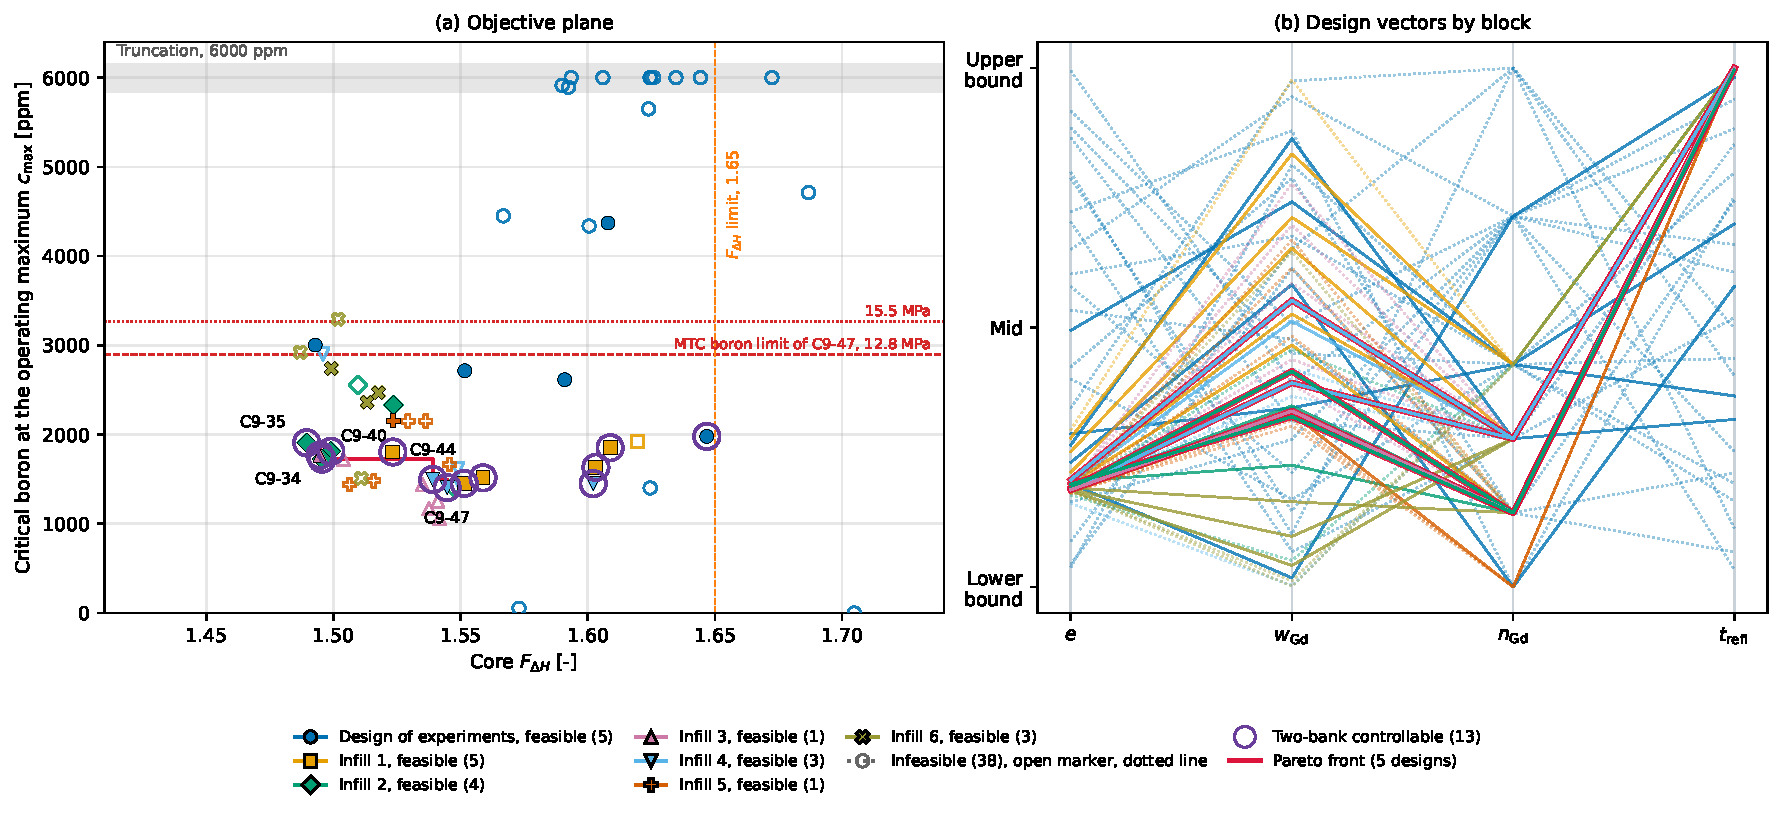
\includegraphics[width=\textwidth]{images/c9_pareto_blocks}
  \caption{Campaign 9: evaluated designs. (a)~Reformulated objective plane. (b)~Design vectors by block.}
  \label{fig:c9-pareto}
\end{figure}

Figure~\ref{fig:c9-pareto}(b) shows where the search went in the
design space:

\begin{itemize}
  \item \textbf{Reflector thickness:} reaches its bound of \SI{5.66}{cm}
        at the first infill iteration and stays there.
  \item \textbf{Enrichment:} decreases from the 2.5 to \SI{13.8}{wt\%}
        of the design of experiments to 4.4 to \SI{5.6}{wt\%} in the
        first infill iteration and to 3.9 to \SI{4.5}{wt\%} from the
        second onward.
  \item \textbf{Gadolinia weight fraction and rod count:} the weight
        fraction stays spread over most of its range to the last
        evaluation, 0.01 to \SI{5.2}{wt\%} in the last iteration, and
        the rod count stays between 12 and 24 rods.
\end{itemize}

The optimiser therefore found no single best gadolinia loading, neither
in weight fraction nor in rod count, and varies the gadolinia along the trade-off with the peaking objective while the enrichment and the reflector thickness
remain at the values on which the search converged.

Three features of the
objective plane stand out before the front itself:

\begin{enumerate}
  \item \textbf{Spread of the feasible designs:} they span 1.490 to 1.647 in
        $F_{\Delta H}$ and 1406 to \SI{4371}{ppm} in $c_\mathrm{max}$, and
        the 5 front members occupy 0.055 of the first range. The boron
        objective separates these designs while the peaking objective
        barely does, which is what makes the front narrow.

  \item \textbf{Designs at the truncation value:} all 8 designs
        at the \SI{6000}{ppm} truncation belong to the design of
        experiments, on which only the bounds of the design space act
        (Section~\ref{sec:meth-loop}), and are infeasible, and every one is rejected on the
        reactivity or the control constraints, so the plateau never
        competes for a place on the front and the truncation never influences the infill selection.

  \item \textbf{Feasible designs above the reference lines:} 2
        feasible designs are above both reference lines, C9-10 at
        \SI{4371}{ppm} and C9-12 at \SI{3003}{ppm}, both of the design
        of experiments (Section~\ref{sec:meth-loop}). Feasibility in the
        optimisation sense and operability are different properties, which
        is why the limit is plotted on the figure and not imposed as a
        constraint.
\end{enumerate}

\begin{table}[!htb]
  \centering
  \begin{threeparttable}
  \caption{Campaign 9: Pareto front in $(F_{\Delta H}, c_\mathrm{max})$.}
  \label{tab:c9-front}
  \small
  \begin{tabular}{@{}lrrrrrrrrc@{}}
    \toprule
    Design & $e$ & Gd$_2$O$_3$ & pins & $t_\mathrm{refl}$ & EFPD\tnote{a} &
    $F_{\Delta H}$ & $c_\mathrm{BOL}$ & $c_\mathrm{max}$ & two \\
     & wt\% & wt\% & & cm & d & & ppm & ppm & banks \\
    \midrule
    C9-47 & 4.46 & 4.42 & 20 & 5.66 & 1947 & 1.545 & 1406 & 1406 & yes \\
    C9-44 & 4.24 & 3.15 & 20 & 5.66 & 1858 & 1.539 & 1334 & 1496 & yes \\
    C9-34 & 4.26 & 3.32 & 16 & 5.66 & 1841 & 1.496 & 1725 & 1725 & yes \\
    C9-40 & 4.23 & 2.71 & 16 & 5.66 & 1870 & 1.495 & 1768 & 1768 & yes \\
    C9-35 & 4.36 & 2.63 & 16 & 5.65 & 1938 & 1.490 & 1908 & 1908 & yes \\
    \bottomrule
  \end{tabular}
  \begin{tablenotes}[flushleft]\footnotesize
    \item[a] Single evaluation, statistical error \SI{29.1}{d}
      (Section~\ref{sec:res-c9-dep-check}).
  \end{tablenotes}
  \end{threeparttable}
\end{table}

Table~\ref{tab:c9-front} supports four results.

\begin{enumerate}
  \item \textbf{Width of the front:} it spans 0.055 in $F_{\Delta H}$ and
        \SI{502}{ppm} in $c_\mathrm{max}$, and every member is between
        4.23 and \SI{4.46}{wt\%}. The Pareto front of the reformulated problem is much narrower than that of the cycle-length formulation.

  \item \textbf{Reflector at its bound:} the reflector is at its upper
        bound of \SI{5.66}{cm} on every member. The limit is set by the
        \SI{90}{cm} vessel inner radius, and the front uses every
        centimetre of reflector the vessel permits.

  \item \textbf{Two-bank control at the operating maximum:} the whole
        front is two-bank controllable at the operating maximum on the
        two-dimensional core. In Campaign 8 3 designs of 60 satisfied that reading, and none of them was on the front. The reformulation
        moves the front into the controllable region.

  \item \textbf{Interpolated concentrations:} the $c_\mathrm{max}$ of
        every front member, 1406 to \SI{1908}{ppm}, is inside the interval
        between the 1000 and \SI{2000}{ppm} solves of the campaign
        evaluation, so it is interpolated between them and the boron
        worth, 6.54 to \SI{6.80}{pcm/ppm}, is the slope between them. No
        front value needs an extrapolation beyond \SI{2000}{ppm}.
\end{enumerate}

Because $c_\mathrm{max}$ is a new objective, measured by the evaluator
from two core solves and a linear interpolation, it was verified on the
5 front designs by a parametric study with all rods out at 0, 1000,
1500 and \SI{2500}{ppm}, with the evaluator and the transport settings
of the campaign, and
Table~\ref{tab:c9-boron-check} compares it with the campaign
evaluation.  The parametric study reproduces the campaign values within
their statistical errors, so the critical boron concentrations of
Table~\ref{tab:c9-front} are confirmed, at beginning of life for all 5
members and at the operating maximum for the 4 without a hump, and the
differential boron worth that the campaign interpolates between 1000
and \SI{2000}{ppm}, 6.54 to \SI{6.80}{pcm/ppm}, is inside the range the
study measures between 1000 and \SI{2500}{ppm}, 6.39 to
\SI{6.89}{pcm/ppm}.

\begin{table}[htbp]
  \centering
  \small
  \caption{Campaign 9 front, all rods out: parametric study in boron concentration against the campaign evaluation.}
  \label{tab:c9-boron-check}
  \begin{tabularx}{\textwidth}{@{}>{\raggedright\arraybackslash}X>{\raggedright\arraybackslash}p{0.25\textwidth}>{\raggedright\arraybackslash}p{0.25\textwidth}@{}}
    \toprule
    Quantity & Parametric study & Campaign evaluation \\
    \midrule
        Concentrations solved [ppm] & 0, 1000, 1500, 2500 & 1000, 2000 \\
    Differential boron worth, 0 to 1000~ppm [pcm/ppm] & 6.83 to 7.10 & -- \\
    Differential boron worth, 1000 to 1500~ppm [pcm/ppm] & 6.62 to 6.89 & -- \\
    Differential boron worth, 1500 to 2500~ppm [pcm/ppm] & 6.39 to 6.74 & -- \\
    Differential boron worth, 1000 to 2000~ppm [pcm/ppm] & -- & 6.54 to 6.80 \\
    Critical concentration $c_\mathrm{BOL}$ [ppm] & 1336 to 1920 & within $-5$ to $+12$ of the study \\
    Multiplication factor at 1000~ppm & -- & within 60~pcm of the study \\
    \bottomrule
  \end{tabularx}
\end{table}

\subsection{Validation of the framework}
\label{sec:res-c9-validation}

The evaluated designs of Campaign 9 are examined with the checks of
Section~\ref{sec:validation-framework}: the leave-one-out
cross-validation and the walk-forward refits of the surrogate
(Section~\ref{sec:validation-surrogate}), and the membership of the front
under the transport noise (Section~\ref{sec:validation-front}).

\begin{itemize}
\item \textbf{Leave-one-out cross-validation
        (Section~\ref{sec:validation-surrogate}):} Table~\ref{tab:c9-cv}
        gives the predictive accuracy of the surrogates of the campaign,
        trained as in the loop on all 60 designs, for the two objectives
        and for the three constraint quantities that decide feasibility.
        The standard deviation $s_z$ of the standardised residuals is 1
        for a calibrated predictor and above 1 for an over-confident one. The table supports three results:
        \begin{itemize}
          \item \textbf{Objectives:} on the 22 feasible designs
                $c_\mathrm{max}$ is predicted within \SI{137}{ppm} with
                $R^2 = 0.959$ and a two-sigma coverage of 0.95, equal to
                the nominal 0.95, so the boron objective is predicted
                accurately and with a calibrated uncertainty where the
                front is. $F_{\Delta H}$ is predicted within 0.024 with
                $R^2 = 0.714$ and a coverage of 0.86, below the nominal,
                with $s_z = 1.28$, so the peaking objective is predicted
                with an error of the size of the spread of the front,
                0.055, and with an uncertainty underestimated by about a
                quarter, and the ordering of the front on the peaking
                axis is not one the surrogate can establish.
          \item \textbf{Cycle length:} the surrogate of the constraint
                that decides feasibility in this campaign has no
                predictive accuracy inside the feasible region, with
                $R^2 = -0.41$, worse than predicting the mean cycle length of the 22 feasible designs,
                and an error of \SI{606}{EFPD} on the 22 feasible
                designs, and over all evaluated designs it
                underestimates its own uncertainty by a factor of 3,
                $s_z = 3.30$. Over all 60 designs it retains the
                ordering, with $R^2 = 0.883$ and $\rho_\mathrm{S} = 0.841$,
                so it predicts in which direction of the design space
                the cycle length increases and not its value near the
                minimum.
          \item \textbf{Feasibility:} with the posterior means the
                surrogates classify 48 of the 60 designs correctly, 80
                per cent, with 6 false positives and 6 false negatives.
                With the feasibility margin of
                Equation~\eqref{eq:feas-margin} at $\kappa = 1.5$ they
                admit only 3 of the 22 feasible designs, consistent with
                the inactive margin of Section~\ref{sec:res-c9-acq}. The
                classification without the margin is therefore adequate
                to guide the search, with its errors balanced between
                the two sides, whereas the margin rejects 19 of the 22
                feasible designs, so at an active constraint it is
                over-conservative and not protective, a restriction of the
                margin rule at an active constraint and not of the
                surrogate, which Section~\ref{sec:concl-future} lists.
        \end{itemize}

\begin{table}[htbp]
  \centering
  \small
  \caption{Campaign 9: leave-one-out cross-validation of the campaign surrogates.}
  \label{tab:c9-cv}
  \setlength{\tabcolsep}{4pt}
  \begin{tabular}{@{}llrrrrrr@{}}
    \toprule
    Output & Designs & RMSE & $R^2$ & $\rho_\mathrm{S}$ & Cov.\ $1\sigma$ & Cov.\ $2\sigma$ & $s_z$ \\
    \midrule
    $F_{\Delta H}$ & all 60 & 0.026 & 0.862 & 0.889 & 0.70 & 0.92 & 1.11 \\
     & feasible 22 & 0.024 & 0.714 & 0.772 & 0.59 & 0.86 & 1.28 \\
    $c_\mathrm{max}$ [ppm] & all 60 & 316 & 0.969 & 0.951 & 0.72 & 0.88 & 1.24 \\
     & feasible 22 & 137 & 0.959 & 0.967 & 0.68 & 0.95 & 1.02 \\
    Cycle length [EFPD] & all 60 & 665 & 0.883 & 0.841 & 0.68 & 0.87 & 3.30 \\
     & feasible 22 & 606 & $-0.409$ & 0.575 & 0.73 & 0.82 & 1.40 \\
    $k_\mathrm{eff}^\mathrm{core}$ & all 60 & 0.0225 & 0.956 & 0.952 & 0.68 & 0.88 & 1.45 \\
     & feasible 22 & 0.0196 & 0.629 & 0.872 & 0.59 & 0.86 & 1.21 \\
    $k_\mathrm{RE}$ & all 60 & 0.0154 & 0.974 & 0.960 & 0.70 & 0.90 & 1.39 \\
     & feasible 22 & 0.0134 & 0.748 & 0.878 & 0.59 & 0.86 & 1.18 \\
    \bottomrule
  \end{tabular}
\end{table}

  \item \textbf{Walk-forward refits of the surrogate
        (Section~\ref{sec:validation-surrogate}):} the walk-forward
        validation refits the Gaussian processes on the evaluations completed before each infill block. Here the same refits, after 24,
        30, 36, 42, 48, 54 and 60 evaluations, are each searched with
        NSGA-II, and Figure~\ref{fig:c9-gp-fronts} draws the front each
        fit predicts against the front the campaign evaluated. The figure measures how the prediction of the surrogate moved, and
        the 6 designs of the last predicted front were then evaluated
        by transport to test whether that prediction was right (third
        item below). The accuracy at the time of each
        acquisition is measured by predicting each block from the evaluations completed before it: pooled over the 36 infill designs, $R^2$ is
        0.556 for $F_{\Delta H}$ and 0.766 for $c_\mathrm{max}$, the
        two-sigma coverage is 0.86 and 0.81, and $c_\mathrm{max}$ is
        overestimated by \SI{88}{ppm} on average with $s_z = 1.87$. The
        comparison of the fronts supports two results.

\begin{figure}[htbp]
  \centering
  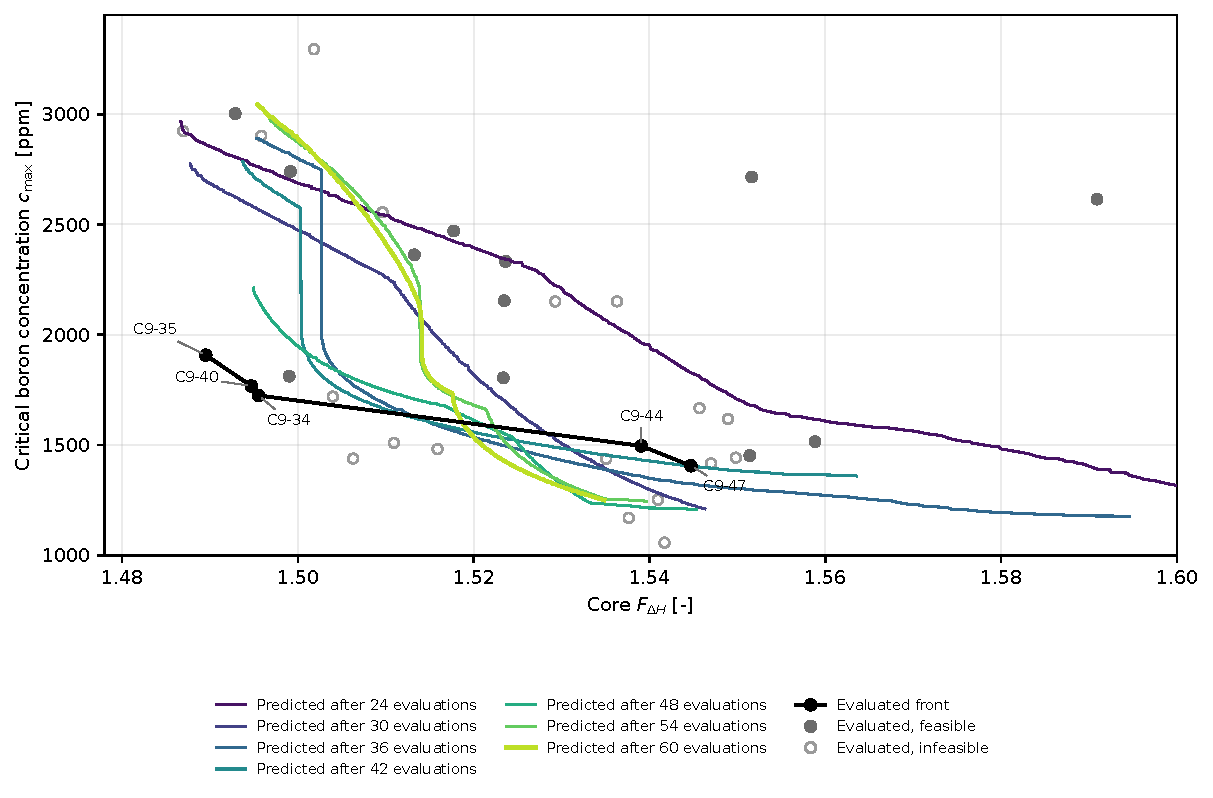
\includegraphics[width=0.85\textwidth]{images/c9_gp_fronts}
  \caption{Campaign 9: fronts predicted by the surrogate and evaluated front.}
  \label{fig:c9-gp-fronts}
\end{figure}

        \begin{enumerate}
          \item \textbf{Narrowing of the predicted front:} after 24
                evaluations it spans 1.487 to 1.640 in $F_{\Delta H}$
                and 995 to \SI{2966}{ppm}, and after 60 it spans 1.495
                to 1.535 and 1250 to \SI{3044}{ppm}, against 1.490 to
                1.545 and 1406 to \SI{1908}{ppm} for the evaluated
                front. The peaking axis converges onto the measured
                range, while the boron axis keeps a tail that no evaluated design reached. The tail consists of designs with almost
                no gadolinia, a region with only 4 evaluated designs below \SI{0.2}{wt\%}, so it is an extrapolation of the
                surrogate.

          \item \textbf{Movement between refits:} normalised, the
                movement of the predicted front is 0.047, 0.038, 0.009,
                0.015, 0.042 and 0.004 over the 6 refits, so the
                prediction was still moving at 54 evaluations, by as
                much as at 36, before settling at the last refit.                 That
                is the same result as the hypervolume, which gains
                \SI{2.1}{\%} in the fourth iteration after 2 nearly
                flat ones.

          \item \textbf{Transport test of the predicted front:} the 6
                designs of the front predicted after 60 evaluations were
                evaluated at the setting of the campaign, with
                $c_\mathrm{max}$ measured by the parametric study in
                boron concentration of the evaluator
                (Section~\ref{sec:meth-c9}), and
                Table~\ref{tab:c9-predicted-front} gives the prediction
                of the surrogate against the value of the evaluator for
                each design. Five of the 6 fail the minimum cycle length,
                by 6 to \SI{87}{d}, and the sixth, at \SI{0.34}{wt\%} of
                gadolinia, is feasible but needs \SI{2749}{ppm}, more
                than any member of the evaluated front. The peaking
                predictions hold within 0.03, whereas the boron
                predictions are optimistic at both ends of the front, by
                \SI{305}{ppm} at zero gadolinia and by \SI{268}{ppm} at
                the low-boron end, so the tail of the predicted front is
                an extrapolation that the transport does not confirm,
                and the predicted front adds no design to the evaluated
                one.
        \end{enumerate}

\begin{table}[htbp]
  \centering
  \footnotesize
  \caption{Campaign 9, front predicted by the surrogate after 60 evaluations: prediction against the campaign evaluation.}
  \label{tab:c9-predicted-front}
  \setlength{\tabcolsep}{3pt}
  \begin{tabular}{@{}rrrrrrrrrrl@{}}
    \toprule
    $e$ & $w_\mathrm{Gd}$ & $n_\mathrm{Gd}$ & \multicolumn{3}{c}{$F_{\Delta H}$} & \multicolumn{3}{c}{$c_\mathrm{max}$ [ppm]} & Cycle & Constraints violated \\
    \cmidrule(lr){4-6}\cmidrule(lr){7-9}
    [wt\%] & [wt\%] & & pred. & eval. & diff. & pred. & eval. & diff. & [d] & \\
    \midrule
    4.18 & 0.00 & 24 & 1.495 & 1.524 & $+0.029$ & 3044 & 3349 & $+305$ & 1797 & $g_{k\max}$, $g_\mathrm{efpd}$, $g_\mathrm{ctrl}$, $g_\mathrm{ctrl,peak}$ \\
    4.21 & 0.34 & 20 & 1.503 & 1.483 & $-0.020$ & 2760 & 2749 & $-11$  & 1871 & none \\
    4.21 & 1.11 & 16 & 1.511 & 1.486 & $-0.025$ & 2342 & 2421 & $+79$  & 1820 & $g_\mathrm{efpd}$ \\
    4.23 & 5.00 & 16 & 1.519 & 1.525 & $+0.006$ & 1584 & 1538 & $-46$  & 1776 & $g_\mathrm{efpd}$ \\
    4.22 & 5.16 & 16 & 1.527 & 1.511 & $-0.016$ & 1360 & 1513 & $+153$ & 1739 & $g_\mathrm{efpd}$ \\
    4.22 & 5.18 & 16 & 1.535 & 1.521 & $-0.014$ & 1250 & 1519 & $+268$ & 1798 & $g_\mathrm{efpd}$ \\
    \bottomrule
  \end{tabular}
\end{table}

  \item \textbf{Membership under the transport noise
        (Section~\ref{sec:validation-front}):} Table~\ref{tab:c9-stability}
        gives the frequency with which each design stays on the front
        when the campaign values of the objectives are perturbed by the
        Monte Carlo noise, 0.012 in $F_{\Delta H}$, the single-solve
        standard deviation measured in Section~\ref{sec:res-c9-peak-noise},
        and \SI{10}{ppm} in $c_\mathrm{max}$, over 2000 replicates. C9-47
        and C9-34 are on the front in at least 99 per cent of the
        replicates, the membership of C9-44, C9-40 and C9-35 is decided by
        the noise, and C9-29 and C9-30 join the front in a quarter to a
        third of the replicates.

\begin{table}[htbp]
  \centering
  \small
  \caption{Campaign 9: front membership frequency under noise.}
  \label{tab:c9-stability}
  \begin{tabular}{@{}lrc@{}}
    \toprule
    Design & Frequency & On the nominal front \\
    \midrule
    C9-47 & 1.00 & yes \\
    C9-34 & 0.99 & yes \\
    C9-44 & 0.54 & yes \\
    C9-40 & 0.54 & yes \\
    C9-35 & 0.42 & yes \\
    C9-29 & 0.34 & no \\
    C9-30 & 0.26 & no \\
    C9-12 & 0.20 & no \\
    \bottomrule
  \end{tabular}
\end{table}

\end{itemize}

\section{Post-analysis of Campaign 9}
\label{sec:res-c9-post}

The post-analysis of Campaign 9 measures, on the designs the campaign
evaluated, what the loop did not evaluate, and it is the final result
of the campaign. Its parts proceed from the checks on the campaign front to the measurements that displace it:

\begin{itemize}
  \item \textbf{Comparison with Campaign 8
        (Section~\ref{sec:res-c9-compare}):} each front scored under the
        objectives of the other campaign.

  \item \textbf{Gadolinia, critical boron concentration and the hump
        (Section~\ref{sec:res-c9-gd}):} the mechanism behind the boron
        objective.

  \item \textbf{Replicates of the depletion
        (Section~\ref{sec:res-c9-dep-check}):} the statistical error of
        the cycle length and the stability of the boron objective.

  \item \textbf{Controllability in three dimensions
        (Section~\ref{sec:res-c9-ctrl3d}):} the front re-solved on the
        three-dimensional core at its own critical concentration.

  \item \textbf{Noise, bias and dimensionality of the peaking
        objective
        (Section~\ref{sec:res-c9-peaking}):} the first correction of
        the front.

  \item \textbf{Axial analyses
        (Section~\ref{sec:res-c9-axial}):} the second correction of the
        front, and the continuation of the search under it.

  \item \textbf{MTC boron limit of each lattice
        (Section~\ref{sec:res-c9-ceiling}):} the operability screen.

  \item \textbf{Final front of Campaign 9
        (Section~\ref{sec:res-c9-readings}):} the front under each
        reading and the final front, followed by the limitations.
\end{itemize}

\subsection{Comparison with Campaign 8}
\label{sec:res-c9-discarded}
\label{sec:res-c9-compare}

The two formulations are compared in both directions. The designs evaluated in Campaign 9 are scored under the Campaign 8 objectives, maximum cycle length
and minimum peaking, with the active constraints of Campaign 8, and the
Campaign 8 candidates of Table~\ref{tab:c8-candidates} are placed on
the Campaign 9 objectives. Table~\ref{tab:c8-c9-compare} gives the
design variables, the objectives of both formulations and the outcome
of each design under the other formulation.

\begin{table}[!htb]
  \centering
  \caption{Campaign 8 candidates and Campaign 9 front: design variables, objectives and outcome under the other formulation.}
  \label{tab:c8-c9-compare}
  \footnotesize
  \setlength{\tabcolsep}{4pt}
  \begin{tabular}{@{}lrrrrrrrl@{}}
    \toprule
    Design & $e$ & $w_\mathrm{Gd}$ & $n_\mathrm{Gd}$ & $t_\mathrm{refl}$ & Cycle & $F_{\Delta H}$ & $c_\mathrm{max}$ & Under the other formulation \\
           & [wt\%] & [wt\%] & & [cm] & [EFPD] & & [ppm] & \\
    \midrule
    C8-47 & 4.39 & 2.88 & 12 & 4.29 & 1941 & 1.510 & 2327 & dominated by C9-34, C9-35, C9-40 \\
    C8-13 & 5.14 & 5.25 & 24 & 3.15 & 2383 & 1.632 & 1697 & dominated by C9-44, C9-47 \\
    C8-53 & 3.45 & 2.92 & 12 & 4.74 & 1142 & 1.524 & 1312 & below the minimum cycle length \\
    \midrule
    C9-47 & 4.46 & 4.42 & 20 & 5.66 & 1947 & 1.545 & 1406 & non-domination rank 3 \\
    C9-44 & 4.24 & 3.15 & 20 & 5.66 & 1858 & 1.539 & 1496 & non-domination rank 4 \\
    C9-34 & 4.26 & 3.32 & 16 & 5.66 & 1841 & 1.496 & 1725 & non-domination rank 3 \\
    C9-40 & 4.23 & 2.71 & 16 & 5.66 & 1870 & 1.495 & 1768 & non-domination rank 2 \\
    C9-35 & 4.36 & 2.63 & 16 & 5.65 & 1938 & 1.490 & 1908 & non-domination rank 1 \\
    \bottomrule
  \end{tabular}
\end{table}

Under the Campaign 8 objectives only one Campaign 9 front member,
C9-35, is non-dominated, so the other front members would not have
been Campaign 8 candidates. In the other direction, the two Campaign 8
candidates that satisfy the minimum cycle length are dominated by
Campaign 9 front members, C8-47 through a lower critical boron
concentration at an equivalent peaking factor and C8-13 on both
objectives, and C8-53 is below the minimum cycle length, so it is not a
candidate under either formulation.

The two campaigns converged on different designs:

\begin{itemize}
  \item \textbf{Distance in the design space:} C8-47 is at a normalised
        distance of 0.401 from the nearest Campaign 9 front member,
        C9-35, and C8-13 at 0.722 from C9-47, 3 to 5 times the minimum
        infill separation of 0.14, so no Campaign 8 candidate is close
        to a Campaign 9 front member.
  \item \textbf{Variable that separates them:} mostly the reflector,
        4.29 and \SI{3.15}{cm} against the upper bound of 5.65 to
        \SI{5.66}{cm} of every Campaign 9 front member.
  \item \textbf{Why the boron objective selects the thickest
        reflector:} a thicker reflector lowers $k_\mathrm{target}$ by
        about \SI{52}{pcm} per centimetre
        (Equation~\eqref{eq:ktarget-c8-fit}), so a design at the minimum
        cycle length reaches it with a lower enrichment and needs less
        boron, which is consistent with the reflector bound being
        active on the whole front.
\end{itemize}

Table~\ref{tab:c8-c9-pairs} compares each Campaign 8 candidate with the
Campaign 9 front members that dominate it, on the three quantities of
both formulations, and gives the statistical error of one evaluation of
each quantity as the scale against which a difference is judged.

\begin{table}[!htb]
  \centering
  \caption{Campaign 9 front against the dominated Campaign 8 candidates: paired differences.}
  \label{tab:c8-c9-pairs}
  \small
  \begin{tabular}{@{}lrrr@{}}
    \toprule
    Pair & $\Delta$Cycle [EFPD] & $\Delta F_{\Delta H}$ & $\Delta c_\mathrm{max}$ [ppm] \\
    \midrule
    C9-35 minus C8-47 & $-3$   & $-0.020$ & $-419$ ($-18\,\%$) \\
    C9-34 minus C8-47 & $-100$ & $-0.014$ & $-602$ ($-26\,\%$) \\
    C9-47 minus C8-13 & $-436$ & $-0.087$ & $-291$ ($-17\,\%$) \\
    \midrule
    Statistical error of one evaluation & 29.1 & 0.014 & 10 \\
    \bottomrule
  \end{tabular}
\end{table}

Read against those errors, the three quantities give three different
outcomes:

\begin{itemize}
  \item \textbf{Critical boron concentration, lower in Campaign 9:}
        every pair differs by 291 to \SI{602}{ppm}, 17 to 26 per cent,
        29 to 60 times the statistical error, the one quantity on which
        the Campaign 9 front is better than both Campaign 8 candidates
        beyond the noise.
  \item \textbf{Peaking factor, equivalent for C8-47:} C9-35 and C9-34
        are lower than C8-47 by 0.020 and 0.014, that is 1.4 and 1.0
        seed standard deviations, so the difference is not significant,
        whereas C9-47 is lower than C8-13 by 0.087, 6.2 standard
        deviations.
  \item \textbf{Cycle length, longer in Campaign 8 only at a cost:}
        C9-35 and C8-47 agree within one statistical error, 1938 and
        \SI{1941}{EFPD}, C9-34 is \SI{100}{EFPD} shorter, and C8-13
        gives \SI{436}{EFPD} more than C9-47 at a peaking factor higher
        by 0.087 and \SI{291}{ppm} more boron.
\end{itemize}

For the requirement of Campaign 9, a cycle of at least \SI{1826}{EFPD}
with the least soluble boron, the Campaign 9 front is therefore the
better result, and Campaign 8 is better only where a cycle beyond the
requirement is valued.

\subsection{Gadolinia, critical boron concentration and the mid-cycle hump}
\label{sec:res-c9-gd}

Section~\ref{sec:res-c9-front} showed that the enrichment and the
reflector converged during Campaign 9, while the gadolinia weight
fraction remained spread over most of its range to the last evaluation
and the number of poisoned pins between 12 and 24. The gadolinia acts
on both terms of the boron objective of Equation~\eqref{eq:c9-cmax} in
opposite directions. It compensates part of the excess reactivity at
beginning of life, which lowers $c_\mathrm{BOL}$, and the reactivity it
suppressed returns as the gadolinium burns out, so the hump
$\Delta\rho_\mathrm{hump}$ of Equation~\eqref{eq:c7-hump} raises
$c_\mathrm{max}$ above $c_\mathrm{BOL}$. Which of the two effects
prevails determines where the front of Campaign 9 is, and the
cycle-length formulation of Campaign 8 did not measure it, because the
gadolinia entered it only as a cost against cycle length.

To separate the gadolinia from the other design variables, the analysis
uses the 16 feasible designs whose enrichment is within
\SI{0.35}{wt\%} of the mean front enrichment of \SI{4.31}{wt\%},
referred to below as the enrichment-matched sample. In this sample the
gadolinia weight fraction spans 0.14 to \SI{5.22}{wt\%},
$c_\mathrm{max}$ spans 1406 to \SI{3003}{ppm}, and all designs but one
have the same reflector. The gadolinia loading is measured by the
weight fraction $w_\mathrm{Gd}$ and by the inventory $I_\mathrm{Gd}$ of
Equation~\eqref{eq:gd-inventory}.

Table~\ref{tab:c9-gd-corr} gives the result. Across the sample a higher
gadolinia loading orders the designs by a lower $c_\mathrm{max}$ and by a
smaller hump, so the two effects act in the same direction. The
concentration decreases by \SI{1597}{ppm} from the most dilute design,
C9-12 at \SI{0.14}{wt\%} and \SI{3003}{ppm}, to C9-47 at
\SI{4.42}{wt\%} and \SI{1406}{ppm}, and above about \SI{2.5}{wt\%} the
hump is below its \SI{400}{pcm} threshold in every design but 2. The
Spearman coefficient of Equation~\eqref{eq:spearman} is used because
the hump vanishes above about \SI{2.5}{wt\%}, so the relation is not
linear, and its $p$ values exclude chance on 16 designs. The weight
fraction and the inventory order the 16 designs almost identically,
with $\rho_S = +0.988$ between them, so the evaluated designs cannot
separate the two measures, and the parametric study in the rod count
of Table~\ref{tab:c9-gdstudy} decides between them.

\begin{table}[htbp]
  \centering
  \caption{Campaign 9 feasible designs at $4.31 \pm \SI{0.35}{wt\%}$: rank correlations with the gadolinia loading.}
  \label{tab:c9-gd-corr}
  \small
  \begin{tabular}{@{}llrr@{}}
    \toprule
    Predictor & Response & Spearman $\rho_S$ & $p$ \\
    \midrule
    Gd weight fraction & $c_\mathrm{max}$ & $-0.932$ & $1.5\times10^{-7}$ \\
    Gd inventory       & $c_\mathrm{max}$ & $-0.953$ & $1.2\times10^{-8}$ \\
    Gd weight fraction & hump             & $-0.723$ & $0.002$ \\
    Gd inventory       & hump             & $-0.684$ & $0.003$ \\
    \bottomrule
  \end{tabular}
\end{table}

Within the enrichment-matched sample the gadolinia loading therefore
governs the boron objective, and a higher loading lowers both terms of
Equation~\eqref{eq:c9-cmax}. It compensates more excess reactivity at
beginning of life, and above about \SI{2.5}{wt\%} it burns out slowly
enough that no hump appears. Four of the 5 front members, at 2.63 to
\SI{4.42}{wt\%}, have no statistically significant hump, and the fifth,
C9-44, has its \SI{3.15}{wt\%} on 20 pins. Because the 16 designs come
from the optimisation and not from a designed experiment, the
enrichment and the pin count also vary within the sample, and the
correlation alone does not isolate the gadolinia. The matched
comparisons of Section~\ref{sec:res-c9-gd-matched} test the relation
with that confounding reduced.

\subsubsection{Matched comparisons}
\label{sec:res-c9-gd-matched}
Two pairs in the sample are matched in gadolinia inventory to within
\SI{7}{\%} and differ in the concentration in each poisoned pin, and
Table~\ref{tab:c9-pairs} lists them. Both pairs have the same reflector
of \SI{5.66}{cm}.

\begin{table}[htbp]
  \centering
  \caption{Campaign 9 feasible designs matched in gadolinia inventory: concentration against hump.}
  \label{tab:c9-pairs}
  \small
  \begin{tabular}{@{}lrrrrrrr@{}}
    \toprule
    Design & $e$ & Gd$_2$O$_3$ & pins & inventory & $c_\mathrm{BOL}$ &
    $c_\mathrm{max}$ & hump \\
     & wt\% & wt\% & & wt\%\,pins & ppm & ppm & pcm \\
    \midrule
    C9-26 & 4.38 & 3.73 & 16 & 59.7 & 1805 & 1805 & 0 \\
    C9-44 & 4.24 & 3.15 & 20 & 62.9 & 1334 & 1496 & $+1093$ \\
    \addlinespace
    C9-32 & 4.42 & 1.88 & 16 & 30.0 & 2121 & 2333 & $+1349$ \\
    C9-51 & 4.18 & 2.68 & 12 & 32.1 & 2154 & 2154 & 0 \\
    \bottomrule
  \end{tabular}
\end{table}

Both pairs point the same way. At matched inventory the design with the
higher concentration in each poisoned pin shows no statistically significant hump, while its
partner shows a hump of 1093 and \SI{1349}{pcm}. The enrichment differs by
0.14 and \SI{0.24}{wt\%} within the pairs, and in both cases the difference
acts against the observed effect, since the design without the hump has
the higher enrichment, so the effect is, if anything, underestimated.

The second pair reverses the ranking. At beginning of life C9-32 needs less
boron, 2121 against \SI{2154}{ppm}. At the operating maximum C9-51 needs
less, 2154 against \SI{2333}{ppm}. At matched inventory and identical
reflector, which of the 2 needs less boron depends on the point of the cycle at
which the 2 designs are compared, which is the clearest single demonstration in this
work that the objective has to be defined at the operating maximum.

A designed study extends the matched comparison to a ladder of 6
lattices at one inventory. Five lattices were built at the enrichment,
reflector thickness and inventory of C9-70, \SI{4.87}{wt\%},
\SI{5.66}{cm} and 88.1, with 12, 16, 24, 32 and 40 poisoned rods, so
that the weight fraction decreases from 7.34 to \SI{2.20}{wt\%} as the
rod count increases, and C9-70 itself, with 20 rods, is the sixth. Each was
evaluated at the setting of the campaign and depleted in 8 layers
(Section~\ref{sec:res-c9-axial}), and Table~\ref{tab:c9-gdstudy} gives
the result.

\begin{table}[htbp]
  \centering
  \small
  \caption{Campaign 9, six lattices at the gadolinia inventory of C9-70: parametric study in the number of gadolinia rods.}
  \label{tab:c9-gdstudy}
  \begin{tabular}{@{}rrrrrrrr@{}}
    \toprule
    Rods & $w_\mathrm{Gd}$ & $\mathrm{EFPD}_\mathrm{asm}$ & Hump & $c_\mathrm{max}$ & $F_{\Delta H}$ & $\mathrm{EFPD}_\mathrm{3D}$ & $\mathrm{EFPD}_\mathrm{3D}/\mathrm{EFPD}_\mathrm{asm}$ \\
    {[--]} & [wt\%] & [d] & [pcm] & [ppm] & [--] & [d] & [--] \\
    \midrule
    12 & 7.34 & 2227 & $-1579$ & 2593 & 1.554 & $1730 \pm 13$ & 0.777 \\
    16 & 5.51 & 2282 & $-1608$ & 2171 & 1.532 & $1827 \pm 8$  & 0.801 \\
    20 & 4.41 & 2280 & $-1010$ & 1840 & 1.539 & $1850 \pm 3$  & 0.811 \\
    24 & 3.67 & 2221 & $+965$  & 1807 & 1.590 & $1842 \pm 8$  & 0.829 \\
    32 & 2.75 & 2278 & $+5532$ & 1887 & 1.595 & $1919 \pm 6$  & 0.842 \\
    40 & 2.20 & 2276 & $+7998$ & 1818 & 1.645 & $1977 \pm 6$  & 0.869 \\
    \bottomrule
  \end{tabular}
\end{table}

The assembly cycle length stays within 2221 to \SI{2282}{d} along the
ladder, as a fixed inventory implies. The critical boron concentration
decreases from \SI{2593}{ppm} at 12 rods to \SI{1807}{ppm} at 24 and
then stays between 1818 and \SI{1887}{ppm}, because the hump increases from
$-1579$ to \SI{+7998}{pcm} as the absorber spreads over more rods and
burns out earlier, while the peaking factor increases from 1.554 to 1.645.
At one inventory the rod count therefore moves the design along the trade-off between the boron and the peaking objectives, and the axially resolved cycle length increases with it, from 1730 to \SI{1977}{d}, a result used in
Section~\ref{sec:res-c9-cont}.

\subsubsection{Mechanism}
\label{sec:res-c9-gd-mechanism}
The hump of Equation~\eqref{eq:c7-hump} is the reactivity gained by
gadolinium burnout minus the reactivity lost by fuel depletion. A
poisoned pin burns from its surface inwards (Section~\ref{sec:bg-gd}),
so a dilute pin loses its absorber before the fuel is appreciably
depleted and produces a hump. Above about \SI{2.5}{wt\%} the burnout is
slow enough for the two effects to cancel, which gives the threshold of
Figure~\ref{fig:c9-hump}.

Figure~\ref{fig:c9-hump} shows the hump of every feasible design
against the gadolinia weight fraction, with the \SI{400}{pcm} threshold
marked. The hump reaches \SI{3430}{pcm} at negligible loading and
decreases below that threshold above \SI{2.5}{wt\%}. Only 3 feasible
designs above that loading retain a statistically significant hump,
C9-1 at \SI{2.76}{wt\%} with \SI{842}{pcm}, outside the
enrichment-matched sample, and C9-44 and C9-42 within it, with
\SI{1093}{pcm} at \SI{3.15}{wt\%} and \SI{512}{pcm} at
\SI{4.10}{wt\%}. All 3 have their gadolinia on 20 or 24 rods instead
of 16, which is the matched comparison of Table~\ref{tab:c9-pairs} seen
from the other side.

\begin{figure}[htbp]
  \centering
  \includegraphics[width=0.7\textwidth]{c9_hump}
  \caption{Campaign 9 feasible designs: mid-cycle hump against the gadolinia weight fraction.}
  \label{fig:c9-hump}
\end{figure}

\subsection{Replicates and fidelity of the depletion on the front}
\label{sec:res-c9-dep-check}

The cycle length, the gadolinium hump and, through the hump, the boron
objective all come from one assembly depletion per design at
$4\,000\times60$ with 20 inactive batches, and 3 statements of this
work rely on that single solve without having been measured:
\begin{enumerate}
  \item the low-fidelity depletion gives the same cycle length as the
        high-fidelity setting of Campaigns 3 and 5,
  \item the front members satisfy the minimum cycle length of
        \SI{1826}{d} with the margins of their single campaign evaluation,
  \item the boron objective is stable under the statistical error of
        the depletion.
\end{enumerate}

The assembly depletion of every front design was repeated with 4
further seeds at the setting of the search and once at the
high-fidelity setting of $16\,000\times120$ with 30 inactive batches.
C9-40 and C9-44, whose margins on the minimum cycle length are close
to zero, were depleted with 4 more seeds, so the study comprises 33
depletions. The beginning-of-life core solves at $100\,000\times170$,
which give the peaking factor, the reactivity window and the boron
points, were not repeated, so the boron objective of each replicate
was computed as in the campaign, from its hump and the boron points of
the campaign.

Table~\ref{tab:c9-dep-replicas} gives the result. The mean combines
the $N-1$ replicates with the campaign evaluation, $N$ independent samples
of the same quantity, and its standard error is the pooled seed standard
deviation divided by $\sqrt{N}$. The column Margin is that mean minus the
minimum cycle length of \SI{1826}{d}, to be compared with the campaign
value minus the same minimum, and the column $t$ is that margin in units
of that standard error.

\label{sec:res-c9-dep-error}%
The pooled seed standard deviation of the cycle length is \SI{29.1}{d},
with 23 degrees of freedom and a 95 per cent range of 22.6 to
\SI{40.8}{d}. It is 1.33 times the \SI{21.9}{d} obtained by propagating
the Monte Carlo errors of the two depletion steps around the crossing
of $k_\mathrm{target}$, because each step inherits the statistical error
of the nuclide inventory of the step before, so every margin of this
section is expressed in units of the measured value. The eight-layer
depletion of Section~\ref{sec:res-c9-cont}, repeated with 5 seeds on
C9-27, C9-70 and C9-88, gives a pooled seed standard deviation of
\SI{15.1}{d} with 12 degrees of freedom, 1.74 times the \SI{8.7}{d}
propagated in the same way. Refitting the ratio model of
Table~\ref{tab:c9-cont-stage2} on the 5-seed means changes its
coefficients by at most 0.1 standard errors, so it was not refitted.

\begin{table}[htbp]
  \centering
  \small
  \caption{Campaign 9 front: seed replicates of the assembly depletion.}
  \label{tab:c9-dep-replicas}
  \begin{tabular}{@{}lrrrrrrrr@{}}
    \toprule
    Design & Campaign & $N$ & Mean & Margin & $t$ & Production & $c_\mathrm{max}$ & s.d. \\
     & [d] & & [d] & [d] & & [d] & [ppm] & [ppm] \\
    \midrule
    C9-47 & 1947 & 5 & 1962 & $+136$ & $+10.4$ & 1970 & 1406 & 0 \\
    C9-35 & 1938 & 5 & 1930 & $+104$ & $+8.0$  & 1931 & 1908 & 0 \\
    C9-34 & 1841 & 5 & 1855 & $+29$  & $+2.2$  & 1841 & 1725 & 0 \\
    C9-40 & 1870 & 9 & 1820 & $-6$   & $-0.7$  & 1822 & 1768 & 34 \\
    C9-44 & 1858 & 9 & 1820 & $-6$   & $-0.6$  & 1805 & 1496 & 34 \\
    \bottomrule
  \end{tabular}
\end{table}

\subsubsection{Cycle length at low and high fidelity}
\label{sec:res-c9-dep-tiers}
The difference between the high-fidelity depletion and the mean of the
low-fidelity replicates is \SI{-2.2}{d} with a standard error of \SI{4.9}{d} over the 5
designs, $t = -0.45$. Nine times more active histories do not move the
cycle length. The low-fidelity setting is adequate for the cycle length,
which is the assumption of the two-tier fidelity strategy of
Section~\ref{sec:meth-fid-settings}.

\subsubsection{Cycle-length margins of the front members}
\label{sec:res-c9-dep-margins}
The standard deviation of \SI{29.1}{d} measured in
Section~\ref{sec:res-c9-dep-error} separates the front into three
groups:

\begin{enumerate}
  \item C9-47 and C9-35 are above the minimum cycle length by 136 and
        \SI{104}{d}, that is 10.4 and 8.0 standard errors. Their
        feasibility in cycle length is established.

  \item C9-34 is above it by \SI{29}{d}, 2.2 standard errors, so it is
        probably feasible.

  \item C9-40 and C9-44 both give \SI{-6}{d} over 9 samples, less than
        one standard error on the infeasible side, and their production
        solves give $-4$ and \SI{-21}{d}. Their cycle length is
        indistinguishable from the minimum, and the campaign margins of $+44$ and \SI{+32}{d} were single samples of a quantity whose
        standard deviation is \SI{29.1}{d}.
\end{enumerate}

This is the constraint-side counterpart of the acquisition behaviour
reported in Section~\ref{sec:res-c9-acq}. Because the cycle-length
constraint is active at the optimum, the optimisation places the
non-dominated designs at the minimum cycle length, and about half of
the designs there are above it only by the statistical error of one
evaluation.
Feasibility at an active constraint cannot be read from a single
evaluation. Section~\ref{sec:res-c9-axial} shows, in addition, that the
margins of this section apply only to the assembly model, since resolving
the axial burnup in three dimensions removes the margin of every front
member.

\subsubsection{Stability of the boron objective}
\label{sec:res-c9-dep-boron}
The replicates measure the hump itself. Pooled over the 5 designs its
seed-to-seed standard deviation is \SI{217}{pcm} on 28 degrees of
freedom, so the \SI{400}{pcm} threshold below which
Equation~\eqref{eq:c9-cmax} replaces the hump by zero is twice that
standard deviation.

Figure~\ref{fig:c9-hump-replicas} shows every depletion of the 5
designs: panel (a) compares the core hump of each depletion with the
\SI{400}{pcm} threshold of Equation~\eqref{eq:c9-cmax}, and panel (b)
gives the resulting $c_\mathrm{max}$ relative to the campaign value.

\begin{figure}[!htb]
  \centering
  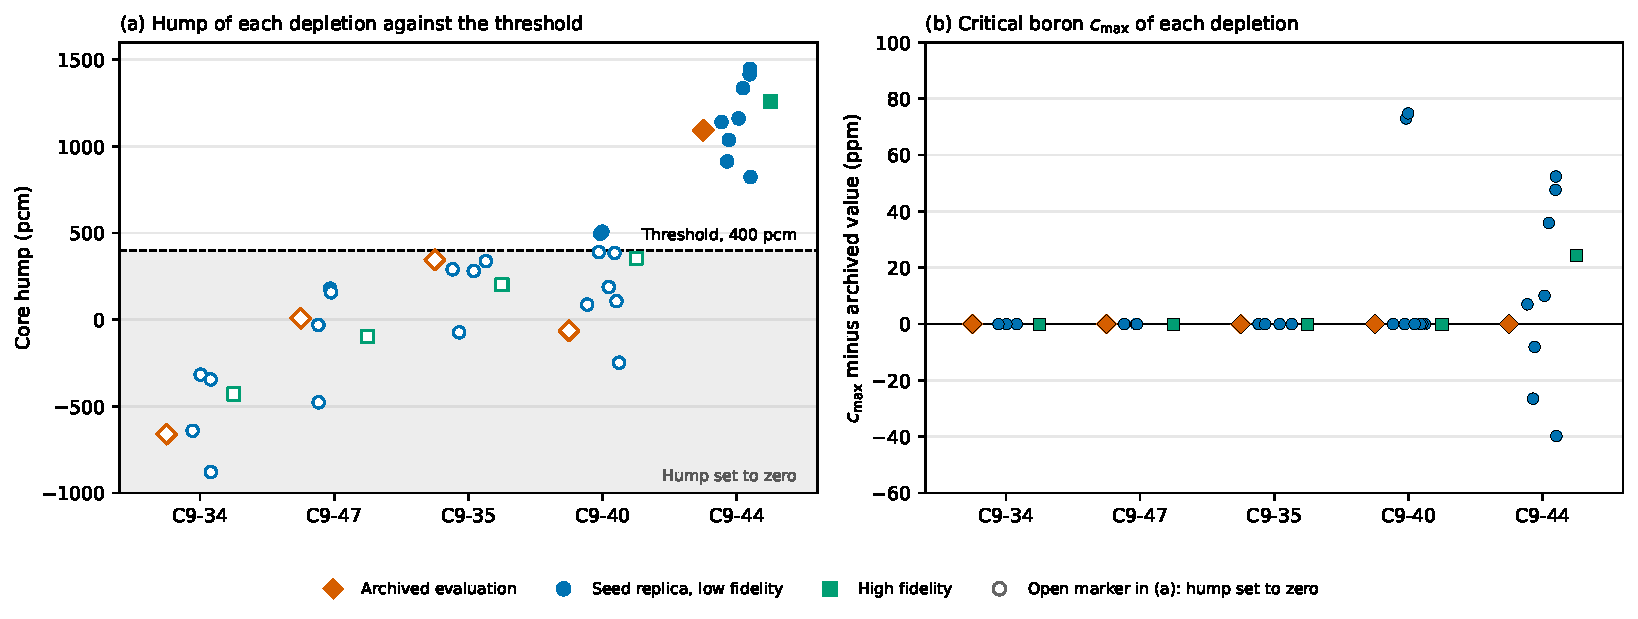
\includegraphics[width=\textwidth]{images/c9_hump_replicas}
  \caption{Campaign 9 front, seed replicates of the depletion: hump against the threshold and critical boron concentration.}
  \label{fig:c9-hump-replicas}
\end{figure}

\noindent The designs are in three groups:

\begin{itemize}
  \item \textbf{Hump below the threshold in every depletion, C9-34,
        C9-47 and C9-35:} the hump is set to zero every time, so
        $c_\mathrm{max}$ reduces to the beginning-of-life concentration,
        which comes from core solves that were not repeated, and it equals the campaign value in every replicate. C9-35 is the closest
        to the threshold, with humps of up to \SI{346}{pcm}.
  \item \textbf{Hump on either side of the threshold, C9-40:} 2 of its
        8 replicates exceed \SI{400}{pcm}, with 496 and \SI{508}{pcm},
        and raise $c_\mathrm{max}$ by about \SI{74}{ppm}. The other depletions give the campaign value.
  \item \textbf{Hump above the threshold in every depletion, C9-44:} the
        hump of 824 to \SI{1448}{pcm} enters $c_\mathrm{max}$ every time,
        which then varies by $-40$ to \SI{+52}{ppm} around the campaign value.
\end{itemize}

The standard deviation of $c_\mathrm{max}$ over the replicates is
\SI{34}{ppm} for C9-40 and C9-44 and zero for the other 3 designs,
and the non-dominated set in $(F_{\Delta H}, c_\mathrm{max})$ is the same 5 designs under the campaign values, under the replicate means and at high
fidelity.

\subsection{Controllability of the front in three dimensions}
\label{sec:res-c9-ctrl3d}
The two-bank reading used throughout the campaign is evaluated on a
two-dimensional core at a fixed \SI{1000}{ppm}, which is neither the
geometry nor the concentration of the operating state. The front was
therefore re-solved on the three-dimensional core model of Section~\ref{sec:reactor-model},
at each design's own critical boron, in 3 rod configurations: all rods
out, the four regulating banks RE1 to RE4 inserted, and the first two
regulating banks inserted.

Table~\ref{tab:c9-ctrl3d} gives the multiplication factors and the
bank worths. The critical concentration of each design is the one that
makes the two-dimensional core critical, so at that concentration the
three-dimensional core is subcritical by the axial leakage alone, and
the axial factor is measured at beginning of life only, because the
confirmation solves are static. Its value on the front and
on the 13 two-bank designs at \SI{1000}{ppm} is consistent with the
1.0289 of Campaign 6 and with the 1.0304 of the withdrawn-rod study of
Section~\ref{sec:res-kt-burnup}. The bank worths are the reactivity
differences from the unrodded value. These solves give three results:

\begin{table}[htbp]
  \centering
  \small
  \caption{Campaign 9 front and two-bank designs, three-dimensional core at beginning of life: multiplication factor and bank worth.}
  \label{tab:c9-ctrl3d}
  \begin{tabular}{@{}lll@{}}
    \toprule
    Quantity & Front, at $c_\mathrm{max}$ & Two-bank designs, \SI{1000}{ppm} \\
    \midrule
    $k_\mathrm{eff}$, all rods out & 0.97014 to 0.97111 & \\
    Subcriticality by axial leakage [pcm] & 2975 to 3078 & \\
    Axial factor & 1.0297 to 1.0308 & 1.0298 to 1.0312 \\
    $k_\mathrm{eff}$, RE1 and RE2 inserted & 0.90453 to 0.90713 & \\
    Two-bank worth [pcm] & 7263 to 7495 & \\
    $k_\mathrm{eff}$, all four banks inserted & 0.83819 to 0.84231 & \\
    Four-bank worth [pcm] & 15\,746 to 16\,245 & 15\,283 to 16\,285 \\
    \bottomrule
  \end{tabular}
\end{table}

\begin{enumerate}
  \item \textbf{Two-bank margin:} every front member is kept
        subcritical by the first two banks alone, with 9228 to
        \SI{9545}{pcm} of margin beyond the operating margin of the
        constraint. The margin is the leakage subcriticality plus the
        two-bank worth, less the operating margin, and it is large because
        at the critical concentration the boron has already compensated
        the whole excess reactivity. The boron objective placed the
        front where this holds, since a design that needs 1406 to
        \SI{1908}{ppm} at its operating maximum has an excess reactivity
        that boron alone compensates.

  \item \textbf{Bank worth in two and in three dimensions:} the two
        banks are worth 7651 to \SI{7812}{pcm} on the two-dimensional
        core and 7263 to \SI{7495}{pcm} on the three-dimensional model,
        4 to 7 per cent less, for the reasons of
        Section~\ref{sec:res-kt-burnup}: the three-dimensional model
        uses the reference rod stack, which absorbs less than the
        full-height B$_4$C of the two-dimensional constraint, and the
        axial leakage changes the flux shape at the banks. The constraint
        therefore credits the banks with 300 to \SI{400}{pcm} more
        worth than the three-dimensional core gives them, an error an
        order of magnitude smaller than the margin it tests.

  \item \textbf{Spread across the front:} the two-bank worth varies by
        3 per cent over designs whose gadolinia loading varies by a
        factor of 1.7, so at their critical concentrations the worth is
        insensitive to the gadolinia loading.
\end{enumerate}

\subsection{Noise, bias and dimensionality of the peaking objective}
\label{sec:res-c9-peaking}

The peaking objective of Campaign 9 is the radial peaking factor
$F_{\Delta H}$ of one two-dimensional core solve per design, at the
campaign statistics of \num{100000} particles and 170 batches with 60
inactive. Because the 5 front members differ by only 0.055 in
$F_{\Delta H}$, an error of 0.01 to 0.03 in that value can change which
designs are non-dominated. Three properties of the value can produce an
error of that size:

\begin{itemize}
  \item \textbf{Statistical noise:} the variation of $F_{\Delta H}$
        between independent solves of the same design.
  \item \textbf{Bias of the estimator:} the upward bias of a maximum
        over noisy pin tallies (Section~\ref{sec:bg-mc}).
  \item \textbf{Dimensionality:} the axial leakage and the axial power
        shape that the two-dimensional solve omits. This is a proxy
        error and not a statistical one like the first two, because the
        two-dimensional core replaces the three-dimensional one, so more
        histories do not reduce it.
\end{itemize}

The fidelity study of Section~\ref{sec:meth-fid-ladder} measured the
assembly estimator of Campaigns 1 to 3, and not the core estimator of
Campaign 9, whose maximum is taken over the pins of the whole core. The
core estimator was therefore measured on the 5 front designs with the
method of Section~\ref{sec:meth-fid-ladder}, and
Section~\ref{sec:res-c9-peak-noise} gives its noise and bias. The 5
front designs were also evaluated again with all rods out at \num{150000} particles and 200 batches with 80
inactive, 2 seeds, on the two-dimensional core and on the
three-dimensional core model of Section~\ref{sec:reactor-model}, which
gives the effect of the fidelity and of the dimensionality.

\subsubsection{Noise and bias of the estimator}
\label{sec:res-c9-peak-noise}
The noise of the estimator determines the smallest statistically
significant difference between two front designs, and its bias
determines how far the campaign values exceed the true peaking factor.
Both were measured after Campaign 9 on the 5 front designs, at
\num{25000}, \num{100000} and \num{400000} particles with the same
batch structure and 8 independent seeds per design and setting.
Table~\ref{tab:fid-ladder-core} gives the result, with the bias at each
setting computed against the extrapolation of
Equation~\eqref{eq:fdh-extrap}.

\begin{table}[htbp]
  \centering
  \begin{threeparttable}
  \caption{Campaign 9 front, core at beginning of life: fidelity study of the peaking estimator.}
  \label{tab:fid-ladder-core}
  \small
  \setlength{\tabcolsep}{4pt}
  \begin{tabular}{@{}lccccc@{}}
    \toprule
    Particles $\times$ batches & Active histories & $s_F$\tnote{a} & $\varepsilon_\mathrm{hot}$\tnote{b} & Bias\tnote{c} & Wall time (s) \\
    \midrule
    $25\,000\times170$ (60)  & $2.75\times10^{6}$ & 0.0249 & 3.9\% & $+0.148$ to $+0.180$ & 36 \\
    $100\,000\times170$ (60) & $1.10\times10^{7}$ & 0.0119 & 2.0\% & $+0.060$ to $+0.077$ & 105 \\
    $400\,000\times170$ (60) & $4.40\times10^{7}$ & 0.0099 & 1.0\% & $+0.035$ to $+0.046$ & 390 \\
    \bottomrule
  \end{tabular}
  \begin{tablenotes}[flushleft]\footnotesize
    \item Inactive batches in parentheses. Five designs and 8 seeds per setting.
    \item[a] Seed-to-seed standard deviation of $F_{\Delta H}$, pooled
      over the 5 designs.
    \item[b] Relative standard error of the hottest-pin tally, mean over
      the calculations of the setting.
    \item[c] Range over the designs of the setting mean minus $F_\infty$ of
      Equation~\eqref{eq:fdh-extrap}.
  \end{tablenotes}
  \end{threeparttable}
\end{table}

The extrapolated values are $1.482 \pm 0.006$ for C9-47,
$1.466 \pm 0.005$ for C9-44, $1.446 \pm 0.006$ for C9-35,
$1.434 \pm 0.006$ for C9-34 and $1.425 \pm 0.004$ for C9-40. The study
supports three results.

\begin{enumerate}
  \item At the campaign setting the bias is $+0.060$ to $+0.077$ on every
        front design, so every campaign value overestimates the peaking
        factor of its design. The bias is about 8 times the $+0.0089$
        of the assembly estimator at $16\,000\times120$, because the
        core maximum is taken over many more pin tallies, each with
        fewer histories. The bias varies by 0.017 across the 5 designs,
        comparable to the differences of 0.009 to 0.020 between front
        designs adjacent in peaking, so it does not
        cancel when 2 front designs are compared and can change their
        order. At the extrapolated values C9-40 is lower than C9-35 in
        peaking by $0.021 \pm 0.007$ and in critical boron
        concentration, so C9-35 is dominated once the bias is removed.

  \item The noise decreases more slowly than $1/\sqrt{N}$, with a fitted
        exponent of $-0.33$, because the maximum moves between pins of
        nearly equal power. At the campaign setting one solve gives
        $F_{\Delta H}$ with a standard deviation $s$ of about 0.012. Two
        designs can be ranked by one solve each only if their peaking
        factors differ by more than twice the standard deviation of the
        difference, about 0.034. Five of the 10
        pairs of front designs differ by only 0.009 to 0.021 at the
        extrapolated values, so one campaign solve cannot establish
        which design of the pair has the lower peaking: C9-47 and C9-44,
        C9-44 and C9-35, C9-34 and C9-40, C9-34 and C9-35, C9-40 and
        C9-35.

  \item The multiplication factor has no measurable fidelity bias. For each
        design the mean $k_\mathrm{eff}$ of the 8 seeds changes by
        5 to \SI{25}{pcm} between the 3 settings, which is
        comparable to the standard error of that mean at the lowest
        setting, 11 to \SI{26}{pcm}, so no systematic dependence on the
        number of histories can be separated from the noise.
\end{enumerate}

The single-solve standard deviation used for every comparison below is
0.011, the value of Table~\ref{tab:fid-ladder-core} interpolated for
the \num{150000} particles and 120 active batches of the confirmation
solves.

The bias was also measured directly on the campaign values of the
front. Table~\ref{tab:c9-peaking} compares the campaign value, a single solve
at the campaign statistics, with the two-dimensional confirmation at
\num{150000} particles and 200 batches with 80 inactive. All 5 shifts
are negative, $-0.005$ to $-0.025$, the direction that the bias of the
estimator predicts, so the campaign values overestimate the peaking
factor of the front by about a quarter of its width on that objective.

\begin{table}[htbp]
  \centering
  \begin{threeparttable}
  \caption{Campaign 9 front, all rods out: radial peaking factor at campaign and confirmation fidelity, in two and three dimensions.}
  \label{tab:c9-peaking}
  \small
  \begin{tabular}{@{}lrrrrrr@{}}
    \toprule
    Design & campaign & 2D conf. & 3D conf. & fidelity & 3D shift &
    3D shift \\
     & $F$ & $F$ & $F$ & shift & & in $\sigma$ \\
    \midrule
    C9-35 & 1.490 & 1.481 & 1.487 & $-0.009$ & $+0.006$ & 0.5 \\
    C9-34 & 1.496 & 1.482 & 1.487 & $-0.014$ & $+0.005$ & 0.5 \\
    C9-40\tnote{a} & 1.495 & 1.490 & 1.460 & $-0.005$ & $-0.030$ & 5.0 \\
    C9-44 & 1.539 & 1.514 & 1.513 & $-0.025$ & $-0.001$ & 0.1 \\
    C9-47 & 1.545 & 1.527 & 1.501 & $-0.018$ & $-0.026$ & 2.4 \\
    \bottomrule
  \end{tabular}
  \begin{tablenotes}[flushleft]\footnotesize
    \item[a] Six seeds per model instead of 2.
  \end{tablenotes}
  \end{threeparttable}
\end{table}

\subsubsection{Dimensionality}
\label{sec:res-c9-peak-3d}
The three-dimensional model adds the axial leakage and the axial power
shape that the two-dimensional objective omits, so the difference
between the two confirmations is the effect of the finite height. The
confirmation values are means of 2 seeds, so the uncertainty of each
difference is about 0.011. The comparison gives three results:

\begin{itemize}
  \item \textbf{The shift is not a constant:} 2 designs move by
        $-0.026$ and $-0.030$, at 2.4 and 5.0 standard deviations of
        their own comparison, while the other 3 move by $+0.005$,
        $+0.006$ and $-0.001$, none of which is statistically
        significant.
  \item \textbf{Mean ratio:} $F^\mathrm{3D}/F^\mathrm{2D}$ is 0.994
        with a standard deviation of 0.012 over the 5 designs.
  \item \textbf{C9-40:} its shift of $-0.030$ is the one that changes
        the front, since it brings C9-40 onto the front and makes C9-35
        dominated (Section~\ref{sec:res-c9-peak-front}). C9-40 was
        therefore evaluated again with 6 seeds per model, which reduces
        the uncertainty of its difference to 0.006 and establishes that
        the shift is not statistical noise.
\end{itemize}

\subsubsection{Consequence for the front}
\label{sec:res-c9-peak-front}
With the two-dimensional confirmation values the non-dominated set of these
5 designs in $(F_{\Delta H}, c_\mathrm{max})$ is C9-34, C9-35, C9-44 and
C9-47, since C9-34 then dominates C9-40. With the three-dimensional values
it becomes C9-34, C9-40 and C9-47. The three changes differ in statistical
significance:

\begin{enumerate}
  \item C9-40 enters the front because its radial peaking factor decreases by
        0.030 between the two models, at 5.0 standard deviations of the
        six-seed comparison. This change is measured.

  \item C9-44 leaves the front because C9-47 improves by 0.026 while C9-44
        does not move, so in three dimensions C9-47 has both the lower
        peaking, 1.501 against 1.513, and the lower boron requirement, 1406
        against \SI{1496}{ppm}. This change is measured.

  \item C9-35 leaves the front because it becomes dominated. Against C9-34
        the dominance is not statistically significant, because both designs reach a peaking
        of 1.487 and the boron requirement alone separates them, 1725
        against \SI{1908}{ppm}. Against C9-40 it is statistically significant at about 2
        standard deviations, with a peaking of 1.460 against 1.487 and a
        boron requirement of 1768 against \SI{1908}{ppm}, so this change depends entirely on the shift of C9-40 in the first item.
\end{enumerate}

Because the three-dimensional shift differs between designs, from
$+0.006$ to $-0.030$, it changes the order of neighbouring front designs
and not only their values, so a correction by one factor common to every
design, as applied before ($L_\mathrm{ax}$, $\mathrm{LF}$), does not
reproduce the three-dimensional front. The 2 seeds of C9-40 differ by 0.016 in
the two-dimensional solve, one standard deviation of the difference of
2 seeds, and the six-seed re-evaluation gives seed standard
deviations of 0.009 in two dimensions and 0.012 in three, consistent
with Table~\ref{tab:fid-ladder-core}.

\subsubsection{The comparison over all evaluated designs}
The comparison with all rods out was extended to all 60 designs, one
solve per design in each model with 2 seeds, and
Table~\ref{tab:c9-peak-all} gives the result. The three-dimensional
correction is not a constant, so it reorders the designs, and the front
recomputed on the three-dimensional peaking changes its membership
except for C9-47, which is on both fronts. The newcomer C9-12 fails the
limit of its own lattice (Section~\ref{sec:res-c9-ceiling}) and cannot
be a candidate whatever its peaking, and part of the change comes from
the fidelity of the campaign solves, through which C9-58 enters the
two-dimensional front. The four quantities that decide the ordering,
the spread of the front, the dimensional shift, the fidelity shift and
the error of the surrogate, are of the same size, so a further campaign
on the peaking objective could not distinguish differences of this
size, and the three-dimensional peaking of C9-47 is reported as a
verified value, inside the 1.65 constraint.

\begin{table}[htbp]
  \centering
  \small
  \caption{Campaign 9, 60 designs, all rods out: three-dimensional against two-dimensional radial peaking factor.}
  \label{tab:c9-peak-all}
  \begin{tabularx}{\textwidth}{@{}>{\raggedright\arraybackslash}p{0.55\textwidth}>{\raggedright\arraybackslash}X@{}}
    \toprule
    Quantity & Value \\
    \midrule
    Three-dimensional minus two-dimensional $F_{\Delta H}$, mean and standard deviation & $-0.023$, 0.017 \\
    Ratio of the two, mean and relative spread & 0.9851, \SI{1.10}{\%} \\
    Rank correlation of the two orderings & 0.941 \\
    Largest rank shift & 14 of 60 \\
    Front of the 22 feasible designs on the two-dimensional peaking & C9-34, C9-35, C9-44, C9-47, C9-58 \\
    Front on the three-dimensional peaking & C9-12, C9-34, C9-40, C9-47 \\
    Fidelity shift, \num{150000} particles against the campaign setting, 41 designs & $-0.016$, standard deviation 0.017, largest $-0.068$ (C9-42) and $-0.037$ (C9-58) \\
    Spread of the front in $F_{\Delta H}$ & 0.055 \\
    Dimensional shift & 0.023 \\
    Fidelity shift & 0.016 \\
    Leave-one-out error of the surrogate on the feasible designs (Table~\ref{tab:c9-cv}) & 0.024 \\
    $F_{\Delta H}$ of C9-47, two and three dimensions & 1.527, 1.501 \\
    \bottomrule
  \end{tabularx}
\end{table}

\subsection{Axial analyses: three-dimensional peaking factor and depletion}
\label{sec:res-c9-axial}

Every campaign obtains the cycle length from one reflective assembly and
$k_\mathrm{target}$ of Equation~\eqref{eq:ktarget-3d}, whose two
leakage factors were measured on fresh fuel, and the burnup check of
Section~\ref{sec:res-kt-burnup} tested only the radial one, on a core
loaded with one uniform depleted nuclide inventory. The end-of-cycle
criterion therefore assumes that the axial power shape of beginning of
life persists over the cycle, that is that the fuel burns uniformly
along its height, the assumption left open when Campaign 8 introduced
the finite-height $k_\mathrm{target}$ (Section~\ref{sec:res-c8}).
Because Campaign 9 changes the formulation and not the depletion
model, the axially resolved depletion stays out of its evaluator, and
this section removes the assumption as a post-analysis of the evaluated
designs.

\subsubsection{Method}
The three-dimensional core model was depleted directly in the layered
form of Section~\ref{sec:meth-axial-dep}, with $N = 1$, 4, 8 and 12
layers. The schedule, the specific power, the boron concentration of
\SI{1000}{ppm} and the all-rods-out configuration are those of the
campaign, and the transport uses $20\,000$ particles per batch over 160
batches, 60 of them inactive.
Figure~\ref{fig:c9-layered-model} shows the model on C9-47, the
design with the most three-dimensional measurements.

\begin{figure}[!htb]
  \centering
  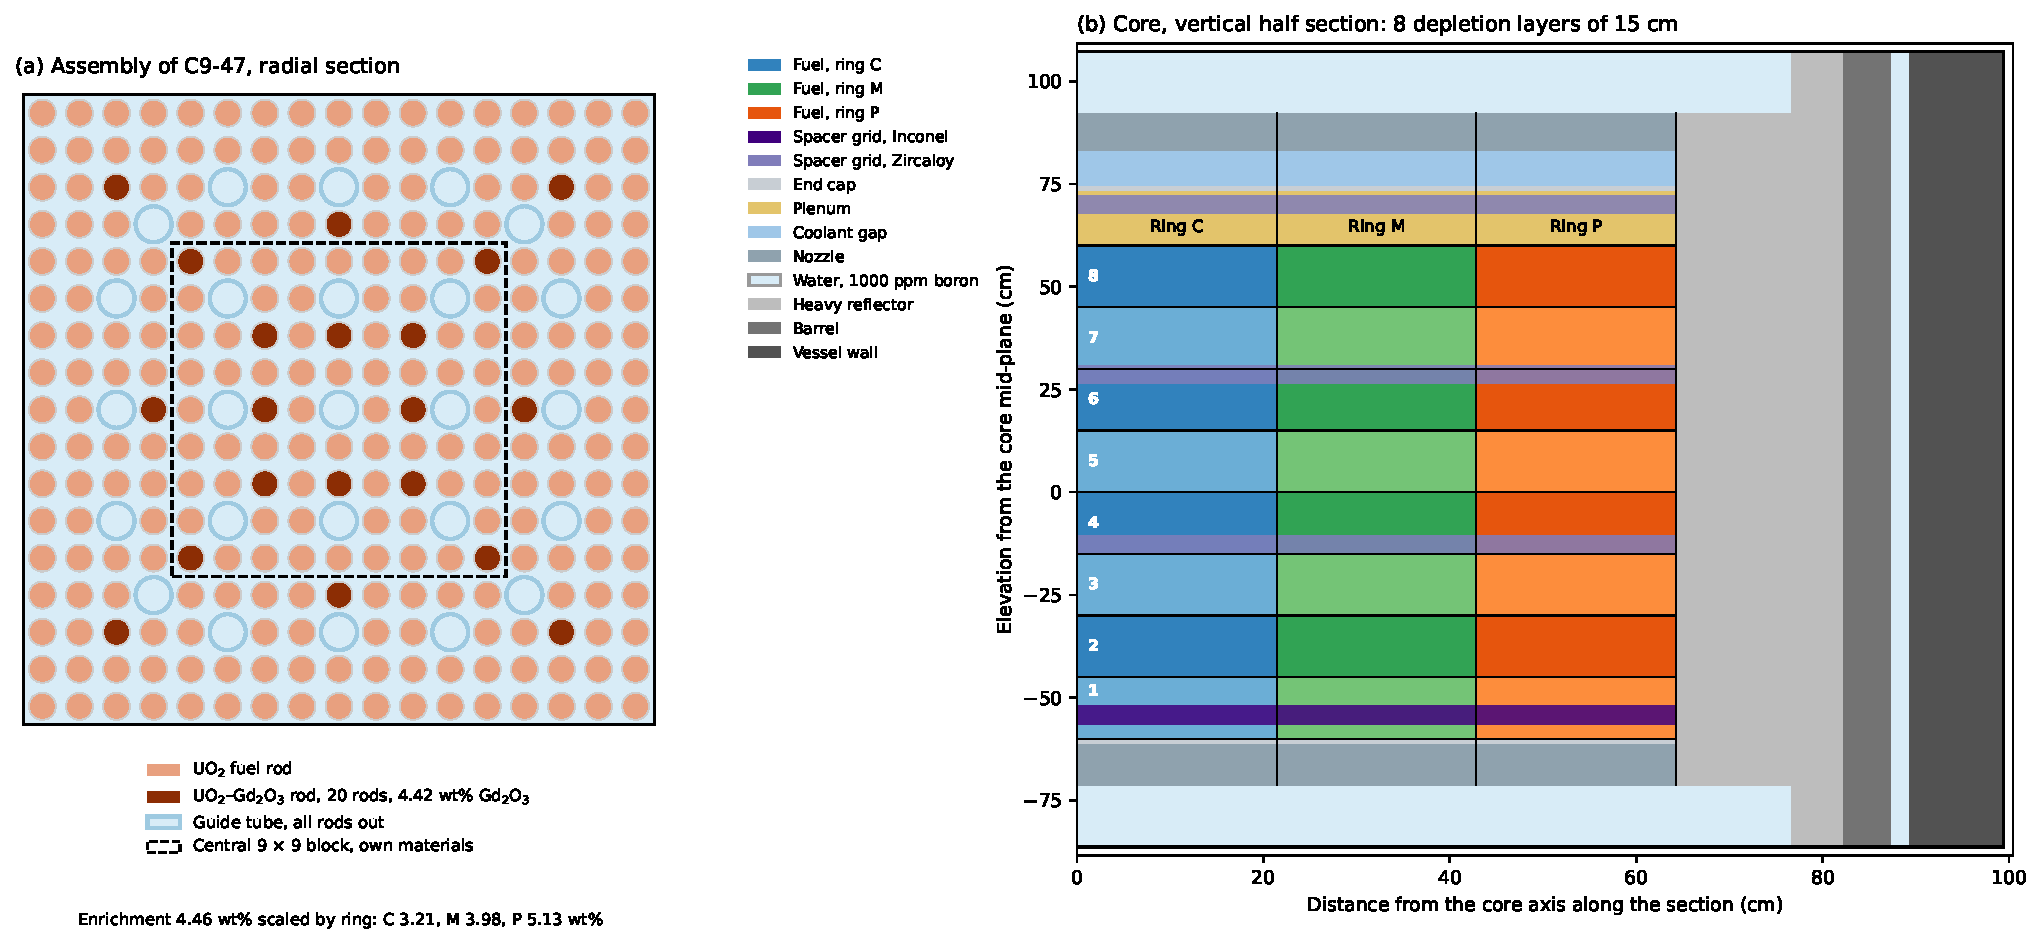
\includegraphics[width=\textwidth]{images/c9_layered_model}
  \caption{Campaign 9, design C9-47: eight-layer depletion model. (a)~Assembly. (b)~Core half section.}
  \label{fig:c9-layered-model}
\end{figure}

The end of cycle is the relative criterion of
Equation~\eqref{eq:axial-eoc} (Section~\ref{sec:meth-axial-dep}), which
isolates the effect of the burnup distribution. An absolute criterion
cannot be used, because at \SI{1000}{ppm} the two-dimensional core of
C9-47 starts at $k = 1.0272$, already below the axial factor of 1.0289.
Only 2 layered depletions were repeated with an independent seed,
C9-70 and C9-88 of the continuation (Section~\ref{sec:res-c9-cont}),
and their differences of $+12$ and \SI{-11}{d} give a seed standard
deviation of about \SI{8}{d} on 2 degrees of freedom, with a 95 per
cent range of 4 to \SI{51}{d}, too wide to be used. The statistical
error of one three-dimensional cycle length is therefore inferred. The error propagated from the two depletion steps around the crossing is
6.1 to \SI{10.2}{d}, and the factor of 1.33 by which the propagation
underestimates the error measured on the assembly depletion
(Section~\ref{sec:res-c9-dep-error}) gives 8 to \SI{14}{d}, about
\SI{12}{d} for C9-47, assuming that the factor measured on the assembly
at $4\,000\times60$ also applies to the three-dimensional depletion.
This error decides whether a number of layers is converged and whether
a design satisfies the minimum cycle length.

\subsubsection{Verification of the model}
The eight-layer three-dimensional model was verified against the
assembly depletion of the campaign in 3 steps, each adding one feature
to the previous model:

\begin{enumerate}
  \item the zoned two-dimensional core adds the radial zoning to the
        assembly,
  \item the three-dimensional core with one layer adds the axial
        leakage at uniform burnup,
  \item the three-dimensional core with 8 layers adds the axial burnup
        distribution.
\end{enumerate}

The four models share the depletion schedule and the specific power of
the campaign, boron at \SI{1000}{ppm}, all control rods withdrawn and
the reference workstation of Table~\ref{tab:hosts}.
Table~\ref{tab:c9-dep-models} gives the set-up in which they differ and
the cycle length that each one computes.

\begin{table}[htbp]
  \centering
  \small
  \caption{Campaign 9, designs C9-47 and C9-35: depletion models of the verification.}
  \label{tab:c9-dep-models}
  \begin{tabularx}{\textwidth}{@{}>{\raggedright\arraybackslash}p{0.15\textwidth}
      *{4}{>{\raggedright\arraybackslash}X}@{}}
    \toprule
    & Assembly & Zoned 2D core & 3D core, one layer & 3D core, 8 layers \\
    \midrule
    Geometry & $17\times17$ assembly, reflective boundaries
      & 32 assemblies in three rings
      & Zoned core, active height \SI{120}{cm}
      & Zoned core, 8 layers of \SI{15}{cm} \\
    Depletable materials & Fuel of the assembly
      & Twelve, one per ring and fuel type
      & The same 12 over the full height
      & Twelve per layer, 96 in all \\
    End of cycle & $k_\infty = k_\mathrm{target}$,
      Equation~\eqref{eq:ktarget-3d}
      & Equation~\eqref{eq:axial-eoc}
      & Equation~\eqref{eq:axial-eoc}
      & Equation~\eqref{eq:axial-eoc} \\
    Transport & $4\,000\times60$, 20 inactive
      & $20\,000\times160$, 60 inactive
      & $20\,000\times160$, 60 inactive
      & $20\,000\times160$, 60 inactive \\
    \midrule
    \multicolumn{5}{@{}l}{\textit{Wall-clock time}} \\
    \quad C9-47 & \SI{7.8}{min} & \SI{0.96}{h} & \SI{0.94}{h} & \SI{0.98}{h} \\
    \quad C9-35 & \SI{7.7}{min} & -- & \SI{0.93}{h} & \SI{1.00}{h} \\
    \midrule
    \multicolumn{5}{@{}l}{\textit{Cycle length [d]}} \\
    \quad C9-47 & 1962 & $1910 \pm 8$ & 1894 & 1573 \\
    \quad C9-35 & 1930 & -- & 1888 & 1641 \\
    \bottomrule
  \end{tabularx}
\end{table}

The four models give the following results:

\begin{itemize}
  \item \textbf{Assembly:} the model of the campaigns, whose
        $k_\mathrm{target}$ contains the table value
        $L_\mathrm{ax} = 1.0289$ with the uncertainty of \SI{80}{pcm} of
        Section~\ref{sec:meth-lax}. The ratio of the two-dimensional
        multiplication factor of the campaign to the three-dimensional
        one at beginning of life averages 1.0301 over the 4 layered
        depletions of C9-47 and 1.0313 over the 2 of C9-35, 114 and
        \SI{238}{pcm} above the table value, so the factor is slightly
        design-dependent, and the relative criterion of
        Equation~\eqref{eq:axial-eoc} is unaffected by it.
  \item \textbf{Zoned two-dimensional core:} the core of the campaign
        core solves, depleted directly with the ratio
        $k_\mathrm{target}/k_{\infty,\mathrm{BOL}} = 0.9697$ of C9-47. It
        gives a cycle \SI{2.6}{\%} shorter than the assembly mean, so the
        assembly depletion represents the radial zoning within a few per
        cent.
  \item \textbf{Three-dimensional core, one layer:} it shortens the
        cycle of C9-47 by \SI{16}{d} against the zoned two-dimensional
        core and that of C9-35 by \SI{2.2}{\%} against its assembly
        mean, so the axial leakage alone shortens the cycle by less than
        \SI{1}{\%}.
  \item \textbf{Three-dimensional core, 8 layers:} each layer burns in
        its own flux, and the cycle is \SI{17}{\%} shorter for C9-47 and
        \SI{13}{\%} for C9-35 than with one layer, so the loss of cycle
        length examined in the rest of this section comes from the axial
        burnup distribution.
\end{itemize}

\subsubsection{Layer convergence and mechanism}
Figure~\ref{fig:c9-axial-layers}(a) gives the cycle length of C9-47
against the number of layers, with the assembly mean, the zoned
two-dimensional core and the minimum cycle length as reference lines.
One layer gives \SI{1894}{d}, 4 give \SI{1673}{d}, 8 give
\SI{1573}{d} and 12 give \SI{1556}{d}, and the change from 8 to 12, \SI{-17}{d}, is about one statistical error of a single
depletion, so 8 layers resolve the effect.

\begin{figure}[htbp]
  \centering
  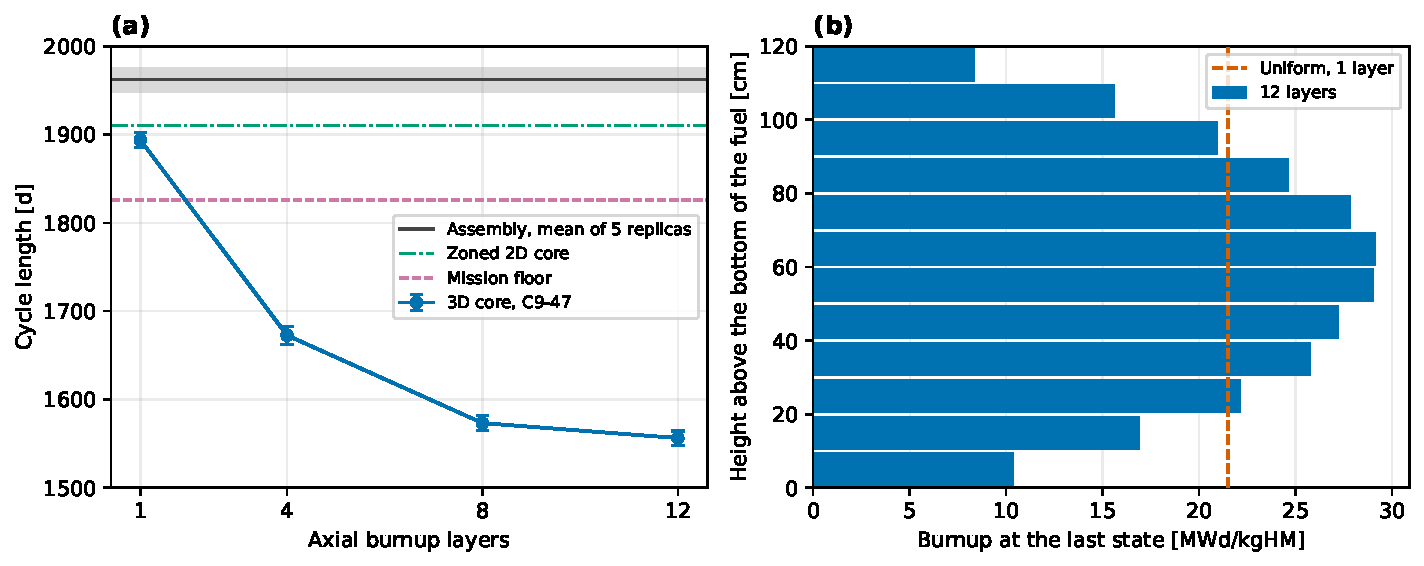
\includegraphics[width=\linewidth]{images/c9_axial_layers}
  \caption{Campaign 9, design C9-47: convergence in the number of burnup layers. (a)~Cycle length. (b)~Axial burnup at the last computed depletion step.}
  \label{fig:c9-axial-layers}
\end{figure}

Figure~\ref{fig:c9-axial-layers}(b) compares the twelve-layer burnup
profile at the last computed depletion step with the uniform assumption
at the same core-average burnup of \SI{21.5}{MWd/kgHM}:

\begin{itemize}
  \item \textbf{Burnup profile:} the 2 central layers reach
        \SI{29.1}{MWd/kgHM}, 1.35 times the average, and the bottom and
        top layers 0.48 and 0.39 times the average.
  \item \textbf{Mechanism:} fuel in the centre has the highest
        importance, since its neutrons have the lowest probability of
        leaking out of the core, so the resolved
        core burns that fuel first and the power moves towards the ends.
        The axial peaking factor $F_z$ decreases from 1.446 to 1.168 over
        the depletion, while with one layer it remains at 1.45. The
        flatter shape places more fission where the leakage is highest,
        so the core loses reactivity faster than with uniform burnup.
  \item \textbf{Burnup limit:} the discharge-burnup limit of
        Section~\ref{sec:meth-atf} applies to the assembly-average
        burnup, which the axial distribution does not change. In the
        zoned two-dimensional depletion of C9-47 the ring with the
        highest power, ring M, has at most 1.17 times its volume share
        of the power, so its average burnup at end of cycle is below
        \SI{23}{MWd/kgHM} against the limit of \SI{55}{MWd/kgHM}. No
        limit of this work applies to the local burnup of the central
        layers, 1.35 times the core average.
\end{itemize}

\subsubsection{Eight designs}
Table~\ref{tab:c9-axial} and Figure~\ref{fig:c9-axial-designs} extend
the study to 8 designs: the front members C9-47 and C9-35, 5
designs that satisfy every constraint of the campaign, and C9-32, the
lowest-peaking design, which a first correction placed within twice
its error of the minimum cycle length and which was depleted after the
others. Three columns of Table~\ref{tab:c9-axial} are specific to this
study:

\begin{itemize}
  \item \textbf{Loss:} the eight-layer cycle length against the
        one-layer one.
  \item \textbf{Margin:} the eight-layer cycle length minus the minimum
        of \SI{1826}{d}, with a statistical error of about \SI{12}{d}.
  \item \textbf{$c_\mathrm{max}$:} recomputed from the gadolinium hump
        of the eight-layer depletion. The hump is below the
        \SI{400}{pcm} threshold in every design except C9-1 and C9-32,
        so for the other 6 designs $c_\mathrm{max}$ equals the campaign
        value.
\end{itemize}

\begin{table}[htbp]
  \centering
  \small
  \caption{Campaign 9, eight designs: cycle length of the three-dimensional depletion.}
  \label{tab:c9-axial}
  \begin{tabular}{@{}lrrrrrrrr@{}}
    \toprule
    Design & Enr. & Gd & Campaign & 1 layer & 8 layers & Loss & Margin & $c_\mathrm{max}$ \\
     & [wt\%] & [wt\%] & [d] & [d] & [d] & [\%] & [d] & [ppm] \\
    \midrule
    C9-1  & 5.51 & 2.76 & 2742 & 2582 & 2271 & $-12.0$ & $+445$ & 2656 \\
    C9-27 & 5.11 & 5.70 & 2373 & 2320 & 1926 & $-17.0$ & $+100$ & 1633 \\
    C9-24 & 5.42 & 6.68 & 2570 &  --  & 1915 &   --    & $+89$  & 1852 \\
    C9-16 & 4.86 & 4.66 & 2283 &  --  & 1909 &   --    & $+83$  & 2715 \\
    C9-11 & 5.26 & 6.91 & 2457 &  --  & 1839 &   --    & $+13$  & 1979 \\
    C9-32 & 4.42 & 1.88 & 1950 &  --  & 1664 &   --    & $-162$ & 2293 \\
    C9-35 & 4.36 & 2.63 & 1938 & 1888 & 1641 & $-13.1$ & $-185$ & 1908 \\
    C9-47 & 4.46 & 4.42 & 1947 & 1894 & 1573 & $-16.9$ & $-253$ & 1406 \\
    \bottomrule
  \end{tabular}
\end{table}

\begin{figure}[htbp]
  \centering
  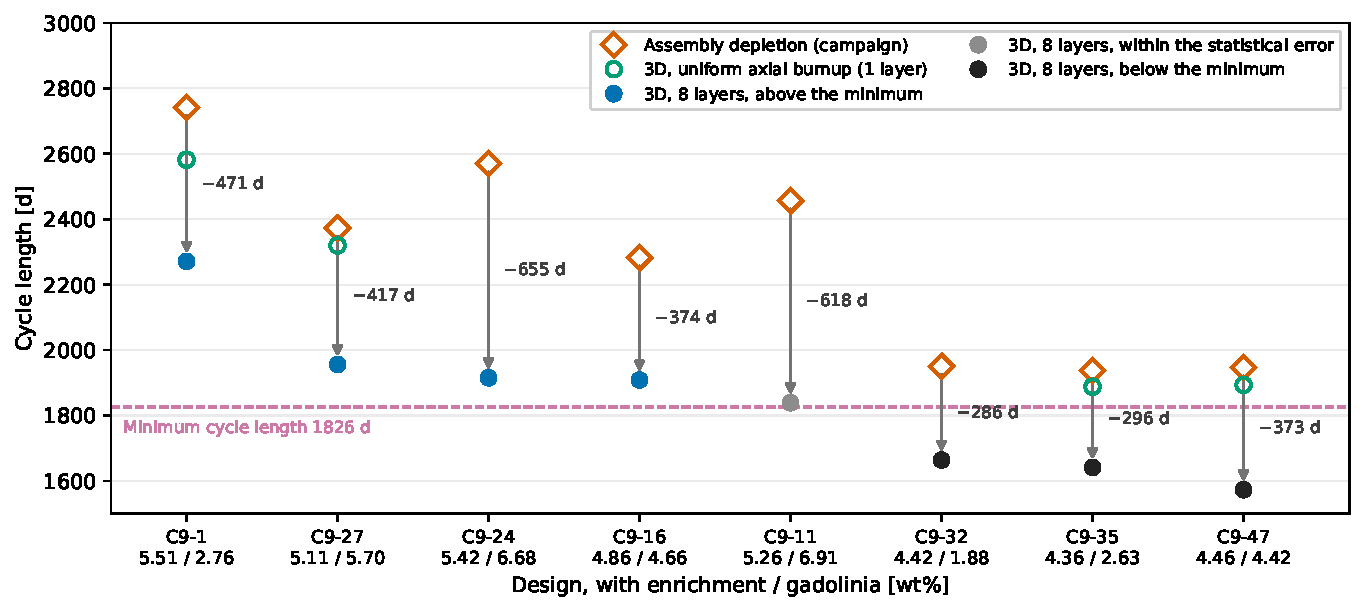
\includegraphics[width=0.9\linewidth]{images/c9_axial_designs}
  \caption{Campaign 9, eight designs: cycle length by depletion model.}
  \label{fig:c9-axial-designs}
\end{figure}

The 8 designs give three results:

\begin{itemize}
  \item \textbf{Loss of cycle length:} resolving the axial burnup
        shortens the cycle by 12.0 to \SI{17.0}{\%} on the 4 designs
        depleted both ways, with a statistical error of about 0.8
        percentage points on one loss, so the spread between designs is
        real.
  \item \textbf{Dependence on the gadolinia:} over all 8 designs the
        ratio of the three-dimensional cycle length to the campaign one
        decreases from 0.85 at 1.9 and \SI{2.6}{wt\%} gadolinia to 0.75
        at 6.7 and \SI{6.9}{wt\%}, with a correlation of $r = -0.86$
        ($p = 0.007$), while the correlation with the enrichment is not
        significant, $r = -0.60$ ($p = 0.11$).
  \item \textbf{Minimum cycle length:} neither front member satisfies
        it once the axial burnup is resolved, C9-47 being \SI{253}{d}
        short and C9-35 \SI{185}{d}. C9-1, C9-27, C9-24 and C9-16
        satisfy it by 445, 130, 89 and \SI{83}{d}, at least 7
        statistical errors, C9-11 is \SI{13}{d} above it, a difference
        that is not statistically significant, and C9-32 is \SI{162}{d}
        short.
\end{itemize}

The cycle lengths of Campaign 8 come from the same single-assembly
depletion, so a reduction to 0.75 to 0.85 of the campaign value would
remove more than the \SI{115}{EFPD}, 6 per cent, by which C8-47 is
above the minimum cycle length (Section~\ref{sec:res-c8-mission}). No
Campaign 8 design was depleted in axial layers, so this conclusion is
an extrapolation.

\subsubsection{The corrected front and the recommended design}
\label{sec:res-c9-axial-front}
Among the 4 designs that satisfy the minimum cycle length in three
dimensions, the non-dominated set in $(F_{\Delta H}, c_\mathrm{max})$
is C9-27, C9-1 and C9-16, and C9-24 is dominated by C9-27 on both
objectives. The three members differ as follows:

\begin{itemize}
  \item \textbf{C9-27:} it needs \SI{1633}{ppm}, the lowest boron of all
        designs that satisfy the minimum cycle length and
        \SI{1130}{ppm} below the MTC boron limit, has no hump,
        $-1791$~pcm before the threshold of
        Equation~\eqref{eq:c9-cmax}, a cycle margin of \SI{100}{d} and
        a peaking factor of 1.603.
  \item \textbf{C9-1:} it has the longest cycle, \SI{445}{d} above the
        minimum, but only \SI{2.76}{wt\%} of gadolinia, and develops a
        hump of \SI{1057}{pcm} in three dimensions against
        \SI{842}{pcm} from the assembly, so its $c_\mathrm{max}$
        increases to \SI{2656}{ppm}, \SI{107}{ppm} below the limit.
  \item \textbf{C9-16:} it has the lowest peaking factor, 1.552, but
        needs \SI{2715}{ppm}, \SI{48}{ppm} below a limit measured on a
        different lattice.
\end{itemize}

C9-27, at \SI{5.11}{wt\%} enrichment and \SI{5.70}{wt\%} gadolinia with
the reflector at its upper bound, is therefore the design this work
recommends.

The members of the corrected front have 4.9 to \SI{5.5}{wt\%}
enrichment, above the 4.2 to \SI{4.5}{wt\%} of the campaign front.
This displacement is expected, because the optimisation had placed the
non-dominated designs at the minimum cycle length computed by the
assembly proxy. The corrected front is a
rescoring of the evaluated designs and not the result of a search, so
an optimum under the resolved rule may be among the designs the search
did not reach, and Section~\ref{sec:res-c9-cont} continues the search
under that rule.

\subsubsection{The mechanism in the form of an axial factor}
Table~\ref{tab:c9-axial-lax} gives the axial burnup correction
$\rho_A$ of Equation~\eqref{eq:axial-rhoA} (Section~\ref{sec:meth-axial-dep}),
the effective axial leakage factor it implies and its accuracy as a
correction, and Figure~\ref{fig:c9-axial-correction} shows the origin of
its shape.

\begin{table}[htbp]
  \centering
  \small
  \caption{Campaign 9, mean of 4 designs: axial burnup correction and effective axial leakage factor.}
  \label{tab:c9-axial-lax}
  \begin{tabular}{@{}lrrrrrrr@{}}
    \toprule
    $B$ [MWd/kgHM] & 0 to 3.5 & 7.5 & 13.5 & 17.5 & 21.5 & 25.5 & 29.5 \\
    \midrule
    $\rho_A$ [pcm] & 0 & 256 & 1497 & 1862 & 2159 & 2091 & 2423 \\
    $L_\mathrm{ax,eff}$ & 1.0289 & 1.0315 & 1.0444 & 1.0482 & 1.0514 & 1.0506 & 1.0541 \\
    \bottomrule
  \end{tabular}
  \vspace{4pt}
  \begin{tabularx}{\textwidth}{@{}>{\raggedright\arraybackslash}p{0.58\textwidth}>{\raggedright\arraybackslash}X@{}}
    \toprule
    Quantity & Value \\
    \midrule
    Onset of the rise of $\rho_A$ & \SI{7.5}{MWd/kgHM} for C9-35, with the least gadolinia, after \SI{17.5}{MWd/kgHM} for C9-24 and C9-11, with the most \\
    Uniform three-dimensional history converted to the layered cycle length, leave-one-out cross-validation over the paired designs & \SI{32}{d} rms \\
    Assembly history converted to the measured three-dimensional cycle length, 7 designs & \SI{276}{d} rms \\
    Assembly against uniform three-dimensional cycle length & 2 to \SI{6}{\%} \\
    Misses on C9-24 and C9-11, 6.68 and \SI{6.91}{wt\%} of gadolinia & 626 and \SI{300}{d} \\
    Burnup steps of the campaign depletion & 4 to \SI{6}{MWd/kgHM} \\
    \bottomrule
  \end{tabularx}
\end{table}

\begin{figure}[htbp]
  \centering
  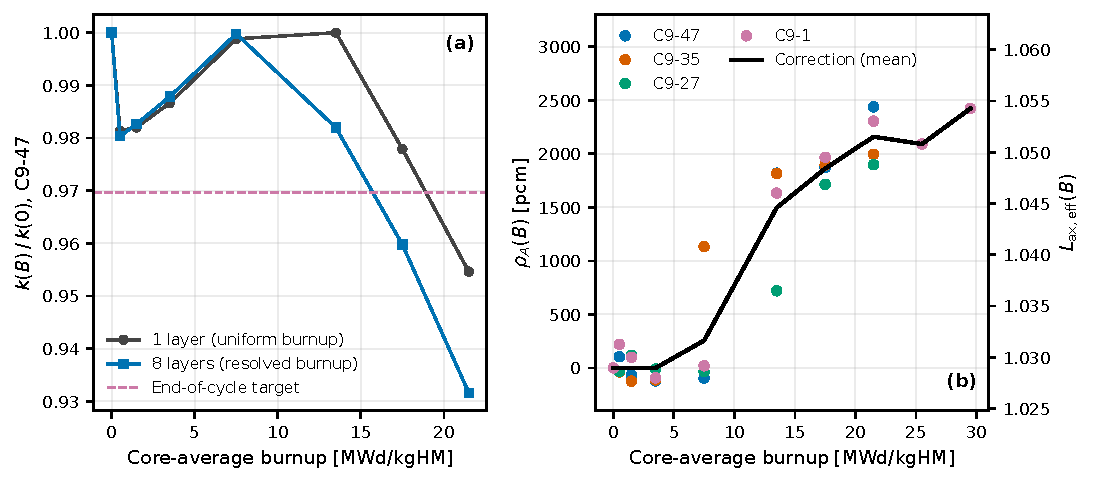
\includegraphics[width=\linewidth]{images/c9_axial_correction}
  \caption{Campaign 9: reactivity loss from the axial burnup. (a)~C9-47 with one and with eight layers. (b)~Four designs and their mean.}
  \label{fig:c9-axial-correction}
\end{figure}

The effective axial factor increases from 1.0289 to 1.0541 as the
gadolinium burns out, because the uniform core burns its gadolinium out
everywhere at once and its multiplication factor increases to a hump near
\SI{13.5}{MWd/kgHM}, whereas in the resolved core the centre burns out
first and the ends last, so the hump is smeared and the faster depletion
of the centre then keeps the gap growing. Two points of the table
qualify the correction. Its value at \SI{25.5}{MWd/kgHM} is below the
one at 21.5, and beyond \SI{21.5}{MWd/kgHM} the mean is computed on C9-1 alone, the only paired design that burned that far, so the correction is
not established past that burnup. Between the two three-dimensional
models the factor is accurate, \SI{32}{d} rms, but as a correction to
the campaign it fails, \SI{276}{d} rms, because the campaign holds
assembly histories and not uniform three-dimensional ones, and because
the rise of the factor is fixed by the burnup at which the calibration
designs burn out their gadolinium, which the burnup steps of the
campaign are too coarse to locate. A burnup-dependent axial factor in
$k_\mathrm{target}$ is therefore the right form for a future campaign,
measured on a burnup grid that resolves the gadolinium burnout and on
the assembly model the campaign depletes.

\subsubsection{The correction that applies to the evaluated designs}
Over the 7 designs depleted in 3D, the ratio of the 3D cycle length to the campaign cycle length is linear in the
gadolinia content.

\begin{equation}
\mathrm{EFPD}_\mathrm{3D} = \mathrm{EFPD}_\mathrm{asm}\,\left(0.9025 - 0.0201\,G\right)
\label{eq:axial-gd}
\end{equation}

\noindent where the symbols have the following meaning.

\begin{itemize}
  \item $\mathrm{EFPD}_\mathrm{3D}$ is the cycle length with axially resolved burnup,
        in d.

  \item $\mathrm{EFPD}_\mathrm{asm}$ is the campaign cycle length from the assembly depletion, in d.

  \item $G$ is the gadolinia content of the design, in wt\%.
\end{itemize}

Table~\ref{tab:c9-axial-gd} gives the accuracy of
Equation~\eqref{eq:axial-gd} under leave-one-out cross-validation and
the minimum assembly cycle length it implies. The equation rescores the
evaluated designs below, while stage 1 of the continuation
(Section~\ref{sec:res-c9-cont}) applies the mean ratio of the 7 designs,
0.805, and admits a design that fails the mission when measured.

\begin{table}[!htb]
  \centering
  \small
  \caption{Campaign 9: accuracy of the gadolinia-dependent cycle-length ratio.}
  \label{tab:c9-axial-gd}
  \begin{tabularx}{\textwidth}{@{}>{\raggedright\arraybackslash}p{0.58\textwidth}>{\raggedright\arraybackslash}X@{}}
    \toprule
    Quantity & Value \\
    \midrule
    Leave-one-out error of Equation~\eqref{eq:axial-gd}, rms and largest & 71 and \SI{107}{d} \\
    Leave-one-out error of a constant ratio, rms & \SI{109}{d} \\
    Range of the fit & 2.6 to \SI{6.9}{wt\%} of gadolinia, 4.4 to \SI{5.5}{wt\%} of enrichment \\
    Minimum assembly cycle length for \SI{1826}{d} in three dimensions at 2.6, 4.4, 5.7 and \SI{6.9}{wt\%} of gadolinia & 2148, 2243, 2317 and \SI{2391}{d} \\
    \bottomrule
  \end{tabularx}
\end{table}

\subsubsection{The peaking factors over the cycle}
Figure~\ref{fig:c9-axial-peaking} gives the peaking of C9-47 over the
cycle in the most detailed calculation, 12 layers, and
Table~\ref{tab:c9-axial-peaking} the values. The flattening of the
axial shape is converged, since the 4-, 8- and 12-layer curves agree
within 0.015 while the one-layer depletion keeps $F_z$ near 1.45
throughout. Neither peaking factor increases above its beginning-of-life
value by more than the seed-to-seed standard deviation over the cycle,
so the peaking constraint evaluated at beginning of life remains
representative of the whole cycle for this design, and only the changes
of $F_{\Delta H}$ are meaningful, since its absolute values at
$20\,000$ particles include the upward bias of a maximum over noisy
tallies.

\begin{table}[htbp]
  \centering
  \small
  \caption{Campaign 9, design C9-47, three-dimensional core: peaking results.}
  \label{tab:c9-axial-peaking}
  \begin{tabularx}{\textwidth}{@{}>{\raggedright\arraybackslash}p{0.55\textwidth}>{\raggedright\arraybackslash}X@{}}
    \toprule
    Quantity & Value \\
    \midrule
    Axial peaking factor $F_z$, 0 to \SI{7.5}{MWd/kgHM} & 1.42 to 1.45 \\
    $F_z$ at 13.5, 17.5 and \SI{21.5}{MWd/kgHM} & 1.30, 1.22, 1.17 \\
    $F_z$ with one layer & about 1.45 throughout \\
    Agreement of the 4-, 8- and 12-layer curves & within 0.015 \\
    Change of $F_{\Delta H}$ through the gadolinium burnout & $-0.15$ to $-0.17$, to 1.50 at \SI{13.5}{MWd/kgHM}, partial recovery after \\
    One-layer against twelve-layer $F_{\Delta H}$ & within the seed-to-seed standard deviation of 0.025 per solve \\
    Bias of the absolute $F_{\Delta H}$ at $20\,000$ particles & $+0.15$ to $+0.2$ \\
    Axial power profile, peak over layer average, at beginning of life and at \SI{21.5}{MWd/kgHM} & 1.45 and about 1.2 \\
    \bottomrule
  \end{tabularx}
\end{table}

\begin{figure}[htbp]
  \centering
  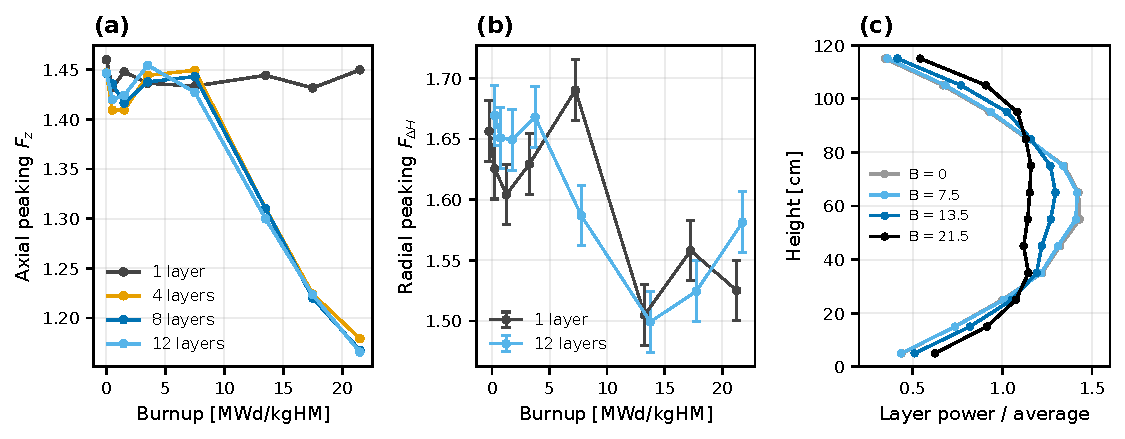
\includegraphics[width=\linewidth]{images/c9_axial_peaking}
  \caption{Campaign 9, design C9-47: peaking over the cycle by number of layers. (a)~Axial peaking factor. (b)~Radial peaking factor. (c)~Axial power profile.}
  \label{fig:c9-axial-peaking}
\end{figure}

\subsubsection{The front before and after the correction}
Figure~\ref{fig:c9-front-2d-3d} rescores every evaluated design with
Equation~\eqref{eq:axial-gd}, using the measured three-dimensional
value where it exists, and redraws the front in
$(F_{\Delta H}, c_\mathrm{max})$. Panel (a) shows all evaluated
designs, and panel (b) the region of the two fronts, where every front
member is named and the designs depleted directly in three dimensions
are circled. Table~\ref{tab:c9-front-corr} gives the two fronts, and
the rescoring gives two results:

\begin{itemize}
  \item \textbf{Independence of the corrected front from
        Equation~\eqref{eq:axial-gd}:} all its members were depleted
        directly, and the 2 projected designs within twice the error of
        the equation of the minimum cycle length are excluded on other
        grounds, C9-12 on boron and C9-32 on its measured cycle, so no
        projected design is within reach of the minimum cycle length.
  \item \textbf{Extrapolation of the equation:} the measured ratio of
        C9-32 agrees with the extrapolation within a third of the
        residual standard deviation, so the equation is valid down to
        \SI{1.88}{wt\%} of gadolinia.
\end{itemize}

\begin{table}[htbp]
  \centering
  \small
  \caption{Campaign 9: front on the assembly and on the axially corrected cycle length.}
  \label{tab:c9-front-corr}
  \begin{tabularx}{\textwidth}{@{}>{\raggedright\arraybackslash}p{0.36\textwidth}>{\raggedright\arraybackslash}X>{\raggedright\arraybackslash}X@{}}
    \toprule
    Quantity & Assembly cycle length & Axially corrected cycle length \\
    \midrule
    Designs feasible & 22 & 6 \\
    Front & C9-35, C9-40, C9-34, C9-44, C9-47 & C9-16, C9-1, C9-27 \\
    Front members depleted directly in 3D & -- & 3 of 3 \\
    Projected designs within twice the error of Equation~\eqref{eq:axial-gd} of the minimum & -- & C9-12, C9-32 \\
    C9-12 & feasible & excluded, \SI{3003}{ppm} above the MTC boron limit \\
    C9-32, depleted with 8 layers & \SI{1950}{d} & \SI{1664}{d}, \SI{162}{d} short; ratio 0.853 measured against 0.865 extrapolated \\
    \bottomrule
  \end{tabularx}
\end{table}

\begin{figure}[htbp]
  \centering
  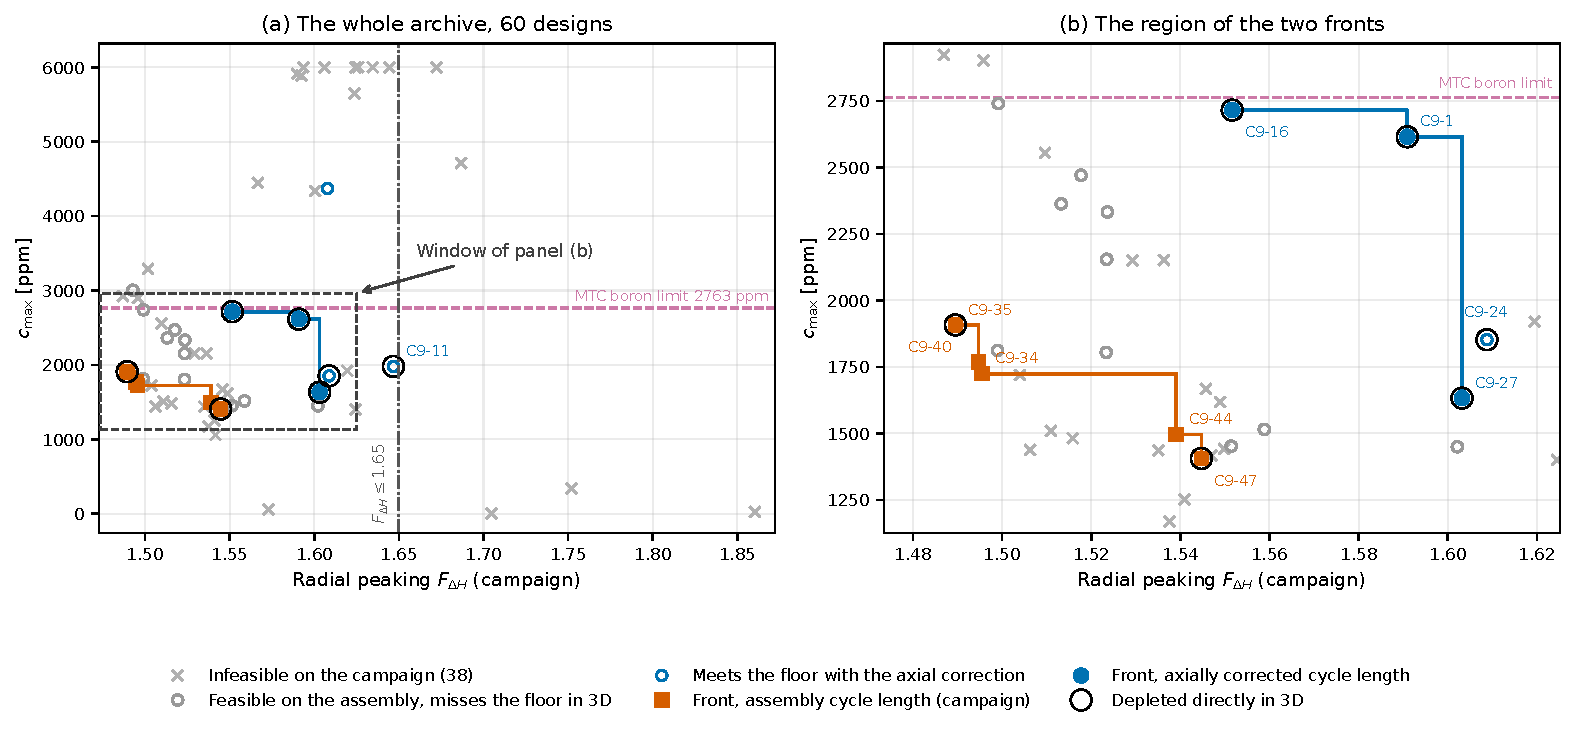
\includegraphics[width=\linewidth]{images/c9_front_2d_3d}
  \caption{Campaign 9: fronts in the objective plane before and after the axial correction. (a)~All evaluated designs. (b)~Region of the two fronts.}
  \label{fig:c9-front-2d-3d}
\end{figure}

\subsubsection{The 2 corrections combined}
\label{sec:res-c9-combined}
Section~\ref{sec:res-c9-peaking} measures the three-dimensional
peaking of all 60 designs and this section measures the axially
resolved cycle length, so the 2 corrections can be applied together
without further transport. Five designs satisfy every constraint that
a correction cannot change, the minimum cycle length with the axially
resolved value and the \SI{2763}{ppm} MTC boron limit: C9-1, C9-11,
C9-16, C9-24 and C9-27, all depleted with 8 axial layers. Scored on the
three-dimensional peaking, their non-dominated set is C9-16 at 1.510 and
\SI{2715}{ppm}, C9-11 at 1.538 and \SI{1979}{ppm}, and C9-27 at 1.565
and \SI{1633}{ppm}, with C9-11 in place of C9-1. The combination gives
three results:

\begin{itemize}
  \item \textbf{The 2 corrections act in opposite directions:} the
        three-dimensional peaking alone selects C9-34, C9-40 and C9-47,
        none of which satisfies the minimum cycle length once the axial
        burnup is resolved, and the evaluated designs with the lowest
        three-dimensional peaking, C9-54, C9-57 and C9-58 at 1.462 to
        1.465, are 188 to \SI{195}{d} short because of their 0.33 to
        \SI{1.31}{wt\%} of gadolinia.
  \item \textbf{C9-27 remains the recommended design:} it needs the
        least boron of any design that satisfies the minimum cycle
        length.
  \item \textbf{C9-11 enters the front:} with a two-dimensional peaking
        of 1.647, at the 1.65 constraint, and a cycle margin of
        \SI{13}{d} that is not statistically significant.
\end{itemize}

\subsubsection{Continuation of the search under the corrected cycle length}
\label{sec:res-c9-cont}
The corrected front of Section~\ref{sec:res-c9-axial-front} is a
rescoring of the designs evaluated in Campaign 9, and the search that
evaluated them placed its front at the minimum cycle length as the
assembly proxy defined it, 15 to 25 per cent above the axially resolved
value. A design that satisfies the mission once the axial burnup is
resolved may therefore be among the designs the search did not reach.
To test this, the search was continued from the 60 evaluations of
Campaign 9 with 6 further infill blocks of 6, blocks 7 to 12 in the
count that starts at the design of experiments, 36 evaluations in all,
C9-60 to C9-95, with every setting of the specification of
Section~\ref{sec:res-c9-formulation} kept. The continuation has two
stages, which differ only in how the axial loss enters the cycle-length
constraint:

\begin{itemize}
  \item \textbf{Stage 1, blocks 7 to 9, C9-60 to C9-77:} a constant
        minimum assembly cycle length,
        $\mathrm{EFPD}_\mathrm{asm} \ge \SI{2270}{d}$, that is
        $1826/0.805$ from the mean ratio
        $\mathrm{EFPD}_\mathrm{3D}/\mathrm{EFPD}_\mathrm{asm}$ of the 7
        designs of Table~\ref{tab:c9-axial}, and the members of the
        resulting front were depleted with 8 axial layers.
  \item \textbf{Stage 2, blocks 10 to 12, C9-78 to C9-95:} seeded with
        all 78 evaluations of stage 1, it requires each unmeasured
        design to satisfy Equation~\eqref{eq:axial-floor}, takes the
        measured cycle for a design already depleted in 8 layers, and
        after each block depletes the unmeasured members of the front
        in 8 layers and refits the model.
\end{itemize}

\begin{equation}
\begin{split}
\mathrm{EFPD}_\mathrm{asm} &\;\ge\; \mathrm{EFPD}_\mathrm{req} \;=\;
\frac{1826}{\hat{r} - \kappa\, s_\mathrm{LOO}},\\
\hat{r} &\;=\; 0.9455 - 0.034337\, w_\mathrm{Gd} - 0.000026\, \Delta\rho_\mathrm{hump}
\end{split}
\label{eq:axial-floor}
\end{equation}

\noindent where $\mathrm{EFPD}_\mathrm{req}$ is the minimum assembly cycle length
of the design, in d, $\hat{r}$ the predicted ratio
$\mathrm{EFPD}_\mathrm{3D}/\mathrm{EFPD}_\mathrm{asm}$, fitted on the 11 designs then
measured in 8 layers, $w_\mathrm{Gd}$ the gadolinia weight fraction,
in wt\%, $\Delta\rho_\mathrm{hump}$ the assembly hump of
Equation~\eqref{eq:c7-hump}, in pcm, $s_\mathrm{LOO} = 0.0164$ the
leave-one-out root mean square error of the fit and $\kappa = 1$ the
margin. Each regressor is truncated to the range of the fitted designs,
1.88 to \SI{6.91}{wt\%} and $-1800$ to \SI{+1247}{pcm}. The 2
regressors are the pair with the smallest leave-one-out error among the
quantities stored by the evaluator (Table~\ref{tab:c9-cont-regressors}).

Table~\ref{tab:c9-cont} gives the two stages. The hypervolumes are on
the reference point of Campaign 9, but each history is computed over
the designs feasible under the rule of its own stage, so the 3
histories are not one convergence history, and the first value of each
stage is that of the designs the stage starts from, scored under the
new rule.

\begin{table}[!htb]
  \centering
  \caption{Campaign 9 continuation: the two stages.}
  \label{tab:c9-cont}
  \small
  \begin{tabularx}{\textwidth}{@{}>{\raggedright\arraybackslash}p{0.11\textwidth}>{\raggedright\arraybackslash}X>{\raggedright\arraybackslash}p{0.17\textwidth}>{\raggedright\arraybackslash}p{0.17\textwidth}>{\raggedright\arraybackslash}p{0.2\textwidth}@{}}
    \toprule
    Stage & Cycle-length constraint & Blocks and designs & Front of the evaluated designs & Hypervolume history \\
    \midrule
    Campaign 9 & $\mathrm{EFPD}_\mathrm{asm} \ge \SI{1826}{d}$ & DOE, 1 to 6; C9-0 to C9-59 & C9-35, C9-40, C9-34, C9-44, C9-47 & 879; 1245, 1291, 1292, 1319, 1319, 1319 \\
    Stage 1 & $\mathrm{EFPD}_\mathrm{asm} \ge \SI{2270}{d}$ & 7 to 9; C9-60 to C9-77 & C9-69, C9-70, C9-72 & 1020; 1061, 1116, 1160 \\
    Stage 2 & Equation~\eqref{eq:axial-floor} for unmeasured designs, the eight-layer cycle for measured ones & 10 to 12; C9-78 to C9-95 & C9-27, C9-69, C9-70 & 1124; 1131, 1131, 1131 \\
    \bottomrule
  \end{tabularx}
\end{table}

The continuation gives four results:

\begin{itemize}
  \item \textbf{Stage 1:} under the constant minimum, 12 of the 78
        designs are feasible and below the MTC boron limit of
        \SI{2763}{ppm}, 5 from Campaign 9 and 7 new. The hypervolume
        increased by 40, 56 and 43 in the 3 blocks, so the stage ended
        on its budget and not on a plateau. Its front is C9-69, C9-70
        and C9-72, at 4.87 to \SI{4.93}{wt\%} enrichment, 4.38 to
        \SI{4.74}{wt\%} gadolinia and the reflector at its upper bound.
        Depleted in 8 layers (Table~\ref{tab:c9-cont-conf}), C9-70
        passes the mission by \SI{24}{d}, 7.8 standard errors of its
        5-seed mean, while C9-72 fails it by \SI{44}{d}, with a ratio
        of 0.777 against the 0.796 it requires. The constant minimum
        therefore admits a design that fails the mission.
  \item \textbf{The quantity the constant minimum omits:} C9-69, C9-70
        and C9-72 have the same enrichment within \SI{0.07}{wt\%} and
        the same gadolinia weight fraction within \SI{0.36}{wt\%}, and
        differ in the number of poisoned pins, 16, 20 and 24. Along this
        sequence $c_\mathrm{max}$ decreases from 2268 to \SI{1559}{ppm},
        $F_{\Delta H}$ increases from 1.526 to 1.594 and the ratio
        decreases from 0.825 to 0.777. The two objectives account for
        the first two changes, and the formulation does not measure the
        third, which decides whether the mission is met.
        Equation~\eqref{eq:axial-gd} also admits the 3 designs, because
        the weight fraction alone predicts a change of 0.007 in the
        ratio against the 0.048 measured.
  \item \textbf{Rule of stage 2:} Table~\ref{tab:c9-cont-regressors}
        gives the leave-one-out error of the ratio for each regressor
        stored by the evaluator, on the 8 designs of
        Table~\ref{tab:c9-axial} and C9-69, C9-70 and C9-72, converted
        to days at an assembly cycle of \SI{2290}{d}. The best
        regressors are the weight fraction and the assembly hump, at
        \SI{38}{d}, while the 4 design variables together over-fit the
        11 designs, so the rule of stage 2 is that pair with a margin of
        one leave-one-out error. The 11 designs do not separate the
        weight fraction from the inventory, and the parametric study of
        Table~\ref{tab:c9-gdstudy} does. At a fixed inventory the ratio
        increases with the rod count by $0.0030 \pm 0.0002$ per rod, 12
        standard errors from the zero slope that the inventory
        predicts, so the weight fraction governs the axial loss. Over
        the 18 designs depleted in 8 layers, every wrong verdict of the
        rule is a design within about \SI{20}{d} of the minimum cycle
        length, so the rule is retained.
  \item \textbf{Stage 2:} Table~\ref{tab:c9-cont-stage2} gives the
        outcome of its 18 evaluations. The front of the measured
        designs, C9-27, C9-69 and C9-70, remained unchanged over the 3
        blocks, and the hypervolume increased by 7 in block 10 and not
        after it. This plateau does not show that the front is optimal,
        because 10 of the 18 evaluations were designs with almost no
        gadolinia whose critical boron concentration exceeds the MTC
        boron limit, which the loop stores and does not constrain, and
        5 were designs that the rule rejects by far more than its own
        error. The 2 designs near the front, C9-85 and C9-88, rejected
        by 9 and \SI{7}{d}, were depleted in 8 layers after the stage
        and fail by 36 and \SI{14}{d} (Table~\ref{tab:c9-cont-conf}),
        so the rule is optimistic at the boundary. Refitted on the 13
        measured designs, the rule keeps its coefficients within the
        noise, but still admits C9-85 and C9-88, which fail, and
        rejects C9-11, which passes.
\end{itemize}

\begin{table}[!htb]
  \centering
  \begin{threeparttable}
  \caption{Campaign 9 continuation: eight-layer depletion.}
  \label{tab:c9-cont-conf}
  \small
  \setlength{\tabcolsep}{3.8pt}
  \begin{tabular}{@{}lrrrrrrrrr@{}}
    \toprule
    Design & $e$ & $w_\mathrm{Gd}$ & $n_\mathrm{Gd}$ & $F_{\Delta H}$ & $c_\mathrm{max}$ & $\mathrm{EFPD}_\mathrm{asm}$ & $\mathrm{EFPD}_\mathrm{3D}$ & $\mathrm{EFPD}_\mathrm{3D}/$ & Margin \\
     & [wt\%] & [wt\%] & & & [ppm] & [d] & [d] & $\mathrm{EFPD}_\mathrm{asm}$ & [d] \\
    \midrule
    C9-27 & 5.11 & 5.70 & 24 & 1.603 & 1633 & 2373 & $1926 \pm 10$\tnote{a} & 0.812 & $+100$ \\
    C9-69 & 4.87 & 4.38 & 16 & 1.526 & 2268 & 2297 & $1895 \pm 7$  & 0.825 & $+69$ \\
    C9-70 & 4.87 & 4.41 & 20 & 1.557 & 1840 & 2280 & $1850 \pm 3$\tnote{a} & 0.811 & $+24$ \\
        C9-72 & 4.93 & 4.74 & 24 & 1.594 & 1559 & 2293 & $1782 \pm 10$ & 0.777 & $-44$ \\
    \addlinespace
    C9-85 & 4.86 & 4.58 & 20 & 1.551 & 1812 & 2290 & $1790 \pm 10$ & 0.782 & $-36$ \\
    C9-88 & 5.00 & 5.52 & 20 & 1.553 & 1859 & 2355 & $1812 \pm 4$\tnote{a} & 0.769 & $-14$ \\
    \bottomrule
  \end{tabular}
  \begin{tablenotes}[flushleft]\footnotesize
    \item[a] Mean of 5 seeds and standard error of the mean.
  \end{tablenotes}
  \end{threeparttable}
\end{table}

\begin{table}[!htb]
  \centering
  \caption{Campaign 9 continuation: leave-one-out error of the cycle-length ratio by regressor.}
  \label{tab:c9-cont-regressors}
  \small
  \begin{tabular}{@{}lrr@{}}
    \toprule
    Regressors of the ratio & \multicolumn{2}{c}{Leave-one-out error [d]} \\
    \cmidrule(l){2-3}
    & 11 designs & 18 designs \\
    \midrule
    None, constant ratio & 89 & 85 \\
    Gadolinia weight fraction $w_\mathrm{Gd}$ & 54 & 47 \\
    Number of poisoned pins $n_\mathrm{Gd}$ & 81 & 92 \\
    Gadolinia inventory $I_\mathrm{Gd}$ & 52 & 62 \\
    $w_\mathrm{Gd}$ and assembly hump $\Delta\rho_\mathrm{hump}$ & 38 & 51 \\
    All 4 design variables & 98 & 59 \\
    \bottomrule
  \end{tabular}
\end{table}

\begin{table}[htbp]
  \centering
  \small
  \caption{Campaign 9 continuation, stage 2: outcome of the 18 evaluations.}
  \label{tab:c9-cont-stage2}
  \begin{tabularx}{\textwidth}{@{}>{\raggedright\arraybackslash}p{0.44\textwidth}>{\raggedright\arraybackslash}X@{}}
    \toprule
    Quantity & Result \\
    \midrule
    Blocks and designs & 10 to 12, C9-78 to C9-95 \\
    Front of the measured designs after each block & C9-27, C9-69, C9-70, unchanged \\
    Hypervolume gain, blocks 10, 11 and 12 & 7, 0, 0 \\
    Evaluations above the MTC boron limit & 10, at 0.08 to \SI{0.77}{wt\%} of gadolinia, 3058 to \SI{3390}{ppm} \\
    Evaluations rejected by the rule by 62 to \SI{216}{d} & 5, C9-80, C9-81, C9-84, C9-89 and C9-92, at 5.2 to \SI{5.6}{wt\%} gadolinia with 16 to 32 rods \\
    Evaluations near the front & 2, C9-85 rejected by \SI{9}{d} and C9-88 by \SI{7}{d} \\
    Eight-layer cycle of C9-85 & $1790 \pm \SI{10}{d}$, ratio 0.782, \SI{36}{d} short at 3.8 standard errors \\
    Eight-layer cycle of C9-88, 5 seeds & $1812 \pm \SI{4}{d}$, ratio 0.769, \SI{14}{d} short at 3.2 standard errors \\
    Ratio model refitted on the 13 measured designs & $\hat{r} = 0.9429 - 0.034396\, w_\mathrm{Gd} - 0.000025\, \Delta\rho_\mathrm{hump}$, leave-one-out error 0.0178, about \SI{41}{d} \\
    Designs the refitted model classifies wrongly & C9-85 and C9-88, admitted and failing, and C9-11, rejected and passing by \SI{13}{d} \\
    \bottomrule
  \end{tabularx}
\end{table}

No correction of the assembly cycle length decides feasibility near
the mission, for four reasons. The leave-one-out error of the best
regression (Table~\ref{tab:c9-cont-regressors}) is 3 to 6 times the
margins of the designs near the mission, while the eight-layer depletion
with 5 seeds resolves the cycle to about \SI{7}{d}. The ratio depends on
the number of poisoned pins at constant gadolinia and enrichment, which
the assembly depletion, executed on one pin arrangement, does not
contain. The central prediction is optimistic at the boundary, and the
margin of one error that rejects C9-85 and C9-88 also rejects C9-11, so
no value of $\kappa$ separates them. The surrogate of the cycle length
has no predictive accuracy in the feasible region
(Table~\ref{tab:c9-cv}), so a correction adjusts the worst-predicted
quantity of the loop.

Near the mission the feasibility check therefore has to be the
eight-layer depletion, applied to the front members and to the designs
that the rule rejects by less than its own error. The continuation
applied it to the front members only, and C9-85 and C9-88 were depleted
separately after the stage, so its front is the front of the designs
measured in 8 layers, and a design that the rule rejected in error
would not have been found.

\subsection{The MTC boron limit of each candidate lattice}
\label{sec:res-c9-ceiling}

Campaign 8 measured one MTC boron limit, on the lattice of C8-47, and
Campaign 9 applied it as a single reference line. The moderator
temperature coefficient responds to a change in moderator density, and
that response depends on the absorber loading of the lattice, which is
a design variable, so one limit cannot apply to every design. Eleven
lattices were therefore scanned on the three-dimensional core model
with the method of Section~\ref{sec:meth-mtc}:

\begin{itemize}
  \item \textbf{Lattices:} every candidate on either peaking front of
        Section~\ref{sec:res-c9-peaking}, C9-57 as a diagnostic
        design, the 2 continuation designs C9-69 and C9-70, and C9-27, the
        recommended design.
  \item \textbf{Scans:} 16 solves per design, with the temperature
        interval of Section~\ref{sec:res-c8-mtc}. Eight lattices were
        scanned at both pressures and 3 at \SI{12.8}{MPa} only, 19
        scans in all.
  \item \textbf{Uncertainty:} for 16 of the 19 scans $\chi^2/\nu$ of
        the three-point fit is below 2. For the other 3 the
        uncertainty is inflated by $\sqrt{\chi^2/\nu}$, to 240 and \SI{173}{ppm}
        for C9-40 and C9-57 against 53 to \SI{109}{ppm} for the other
        designs.
\end{itemize}

Table~\ref{tab:c9-ceilings} gives the 11 lattices, ordered by the
gadolinia inventory $I_\mathrm{Gd}$ of
Equation~\eqref{eq:gd-inventory}, with the margin as the limit minus the
critical boron concentration $c_\mathrm{max}$ of the same design, and
Figure~\ref{fig:c9-ceiling-2p} plots the limits against the gadolinia
loading. Where the coefficient is still negative at the last scanned
concentration of \SI{3000}{ppm}, the limit is the extrapolation of the
three-point fit and is marked as such.

\begin{table}[htbp]
  \centering
  \caption{Campaign 9 lattices: MTC boron limit and operating margin at both pressures.}
  \label{tab:c9-ceilings}\label{tab:c9-ceilings-p155}
  \small
  \setlength{\tabcolsep}{4.2pt}
  \begin{tabular}{@{}lrrrrrrrr@{}}
    \toprule
    & & & & \multicolumn{2}{c}{\SI{12.8}{MPa}} & \multicolumn{2}{c}{\SI{15.5}{MPa}} \\
    \cmidrule(lr){5-6}\cmidrule(lr){7-8}
    Design & Gd & rods & inventory & limit & margin & limit & margin \\
    {[--]} & [wt\%] & [--] & [--] & [ppm] & [ppm] & [ppm] & [ppm] \\
    \midrule
    C9-12 & 0.14 & 32 & 4.5  & $2091 \pm 69$  & $-912$  & $2522 \pm 46$  & $-481$ \\
    C9-57 & 0.78 & 20 & 15.6 & $2278 \pm 173$ & $-193$  & --             & -- \\
    C9-58 & 1.31 & 16 & 21.0 & $2483 \pm 53$  & $+120$  & $2739 \pm 89$  & $+376$ \\
    C9-35 & 2.63 & 16 & 42.0 & $2617 \pm 69$  & $+710$  & --             & -- \\
    C9-40 & 2.71 & 16 & 43.4 & $2651 \pm 240$ & $+883$  & --             & -- \\
    C9-34 & 3.32 & 16 & 53.2 & $2752 \pm 97$  & $+1027$ & $3092 \pm 106$ & $+1367$ \\
    C9-44 & 3.15 & 20 & 62.9 & $2858 \pm 109$ & $+1362$ & $2931 \pm 80$  & $+1435$ \\
        C9-47 & 4.42 & 20 & 88.4 & $2897 \pm 99$  & $+1491$ & $3266 \pm 75$  & $+1860$ \\
    \addlinespace
        C9-69 & 4.38 & 16 & 70.1 & $2867 \pm 115$ & $+599$  & $3271 \pm 113^\dagger$ & $+1002$ \\
        C9-70 & 4.41 & 20 & 88.1 & $3018 \pm 102^\dagger$ & $+1178$ & $3299 \pm 138^\dagger$ & $+1459$ \\
    C9-27 & 5.70 & 24 & 136.7 & $3128 \pm 111^\dagger$ & $+1495$ & $3384 \pm 111^\dagger$ & $+1752$ \\
    \bottomrule
    \multicolumn{8}{@{}l}{\footnotesize $^\dagger$Extrapolated beyond the scanned \SI{3000}{ppm}.}
  \end{tabular}
\end{table}

\begin{figure}[htbp]
  \centering
  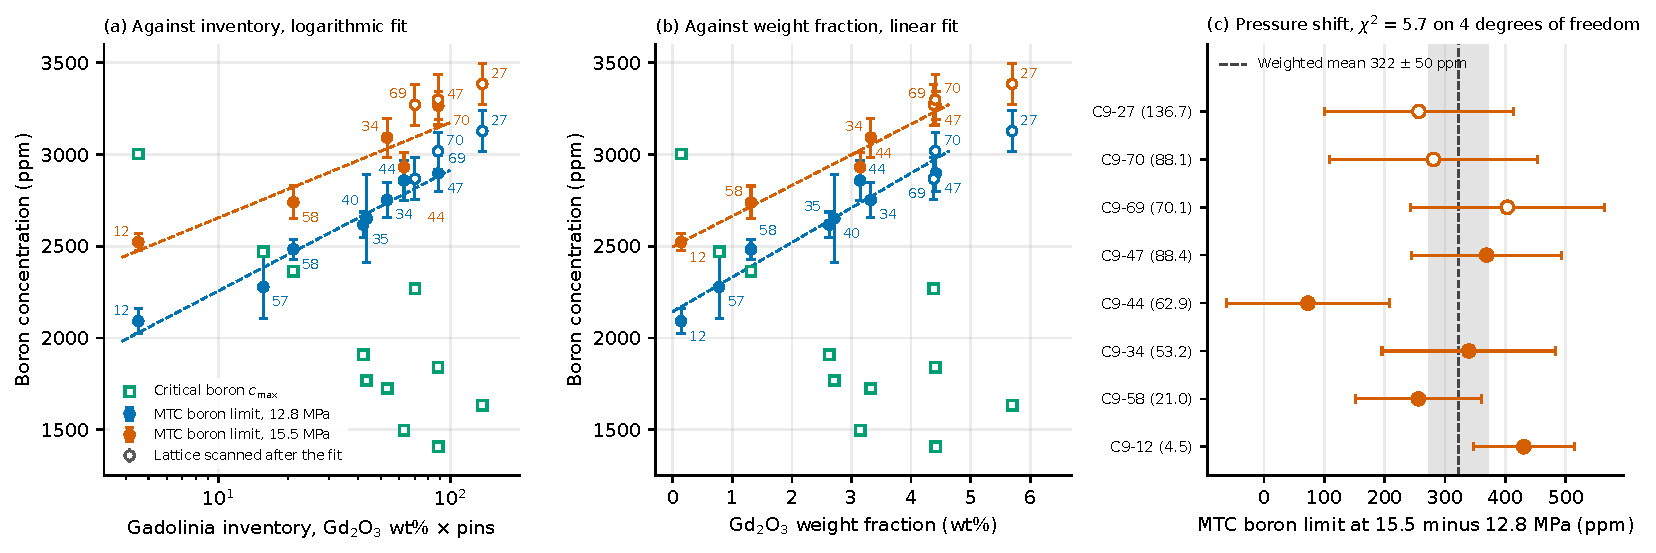
\includegraphics[width=\textwidth]{images/c9_ceiling_two_pressures}
  \caption{Campaign 9 lattices: MTC boron limit at both pressures against the gadolinia loading.}
  \label{fig:c9-ceiling-2p}
\end{figure}

The limit increases with the gadolinia loading at both pressures. Over
the 8 lattices scanned before the continuation, 5 of them at
\SI{15.5}{MPa}, the Spearman coefficient against the inventory is 1.000
at \SI{12.8}{MPa} and 0.900 at \SI{15.5}{MPa}, and against the number
of gadolinia pins alone $-0.07$ and $-0.10$. An unweighted logarithmic
fit in the inventory over the same lattices describes the dependence.

\begin{equation}
  c_\mathrm{MTC}(I_\mathrm{Gd}) = a \ln I_\mathrm{Gd} + b
  \label{eq:mtc-ceiling-fit}
\end{equation}

\noindent where the symbols have the following meaning.

\begin{itemize}
  \item $c_\mathrm{MTC}$ is the boron concentration at which the
        moderator temperature coefficient crosses zero, in ppm.
  \item $I_\mathrm{Gd}$ is the gadolinia inventory of
        Equation~\eqref{eq:gd-inventory}, entered as a pure number.
  \item $a$ is the slope, \SI{287}{ppm} at \SI{12.8}{MPa} and
        \SI{226}{ppm} at \SI{15.5}{MPa}.
  \item $b$ is the intercept, \SI{1595}{ppm} at \SI{12.8}{MPa} and
        \SI{2134}{ppm} at \SI{15.5}{MPa}.
\end{itemize}

The root mean square residual of the fit is \SI{55}{ppm} at
\SI{12.8}{MPa} and \SI{96}{ppm} at \SI{15.5}{MPa}. The inventory and
the weight fraction rank the lattices identically except C9-34 and
C9-44, so the present data do not show which of the two governs the
limit. The fit was tested on C9-69, C9-70 and C9-27, the 3 lattices
scanned after it, shown with open markers in
Figure~\ref{fig:c9-ceiling-2p}. At \SI{12.8}{MPa} it predicts 2815,
2880 and \SI{3006}{ppm}, within 1.4 standard deviations of the measured
limits, and at \SI{15.5}{MPa} it underestimates them by 1.1 to 1.6
standard deviations, so it predicts the limit of a new lattice within 2
standard deviations at both pressures.

The scans give three further results:

\begin{itemize}
  \item \textbf{Pressure:} the limit is higher at \SI{15.5}{MPa} than at
        \SI{12.8}{MPa} for each of the 5 lattices scanned at both
        pressures before the continuation, by \SI{322(50)}{ppm} on
        average, with a scatter that statistical noise alone produces
        with a probability of $p = 0.22$, and the 3 lattices scanned
        after it agree, with shifts of $404 \pm 161$, $281 \pm 172$ and
        $256 \pm \SI{157}{ppm}$ for C9-69, C9-70 and C9-27.
        The same lattices satisfy their limit at both pressures, so
        \SI{12.8}{MPa} is the binding pressure.
  \item \textbf{Fidelity of the comparison:} the limit is measured on
        the three-dimensional core and $c_\mathrm{max}$ on the
        two-dimensional one. On C9-47 the three-dimensional limit is
        $430 \pm \SI{145}{ppm}$ above the two-dimensional one at
        \SI{12.8}{MPa}, and at the two-dimensional critical
        concentration the three-dimensional core of the 5 front designs
        is 3001 to \SI{3027}{pcm} less reactive, 445 to \SI{459}{ppm}
        of boron. The quoted margins are therefore conservative by about
        \SI{450}{ppm}, since the margin of C9-47 is \SI{1491}{ppm} as
        quoted, \SI{1950}{ppm} fully in three dimensions and
        \SI{1060}{ppm} fully in two. The comparison is not corrected,
        because a correction would mix a measured quantity with an
        inferred one.
  \item \textbf{Lattices that satisfy their limit:} at \SI{12.8}{MPa}
        C9-27, C9-47, C9-44, C9-70, C9-34, C9-40, C9-35 and C9-69
        satisfy it by 599 to \SI{1495}{ppm}, at 3.7 standard deviations
        or more. C9-58
        satisfies it by \SI{120}{ppm}, at 2.3 standard deviations, so
        its operability is not established. C9-57 fails by
        \SI{193}{ppm}, within the fidelity mismatch, so it is undecided
        and marks the boundary at roughly \SI{1}{wt\%} of gadolinia.
        C9-12 fails by \SI{912}{ppm}, and it still fails by about
        \SI{460}{ppm} with both sides on the three-dimensional core.
\end{itemize}

In the 11 lattices the effect of the inventory cannot be separated
from that of the reflector thickness, because the reflector is at its
bound for 10 of them. The logarithmic law of
Equation~\eqref{eq:mtc-ceiling-fit} is therefore valid only inside the
converged region of this campaign and should not be extrapolated
outside it.

\subsection{Final front of Campaign 9}
\label{sec:res-c9-readings}\label{sec:res-c9-cont-front}

The corrections of Sections~\ref{sec:res-c9-peaking} and
\ref{sec:res-c9-axial} and the continuation of the search give the same
evaluated designs a different front under each reading.
Table~\ref{tab:c9-readings} gives the 5 readings. For each reading it
names the model of the peaking factor and the model of the cycle length,
the non-dominated set in $(F_{\Delta H}, c_\mathrm{max})$ among the
designs feasible under that reading, and whether its members satisfy the
minimum cycle length once the axial burnup is resolved.
Figure~\ref{fig:c9-readings} shows the readings over the designs
evaluated in Campaign 9 and in the 2 stages of the continuation, with
the MTC boron limit of C8-47, which the readings apply, and the limit of
the C9-27 lattice (Section~\ref{sec:res-c9-ceiling}). The first two
readings keep the assembly cycle length, so their fronts are at the
minimum cycle length where the assembly proxy placed them, and no
member of either satisfies that minimum in three dimensions. The last
three use the axially resolved cycle length, and the last is the final
front of this work.

\begin{table}[htbp]
  \centering
  \small
  \begin{threeparttable}
  \caption{Campaign 9: front under each reading of the evaluated designs.}
  \label{tab:c9-readings}
  \begin{tabularx}{\textwidth}{@{}>{\raggedright\arraybackslash}p{0.19\textwidth}>{\raggedright\arraybackslash}p{0.15\textwidth}>{\raggedright\arraybackslash}p{0.13\textwidth}>{\raggedright\arraybackslash}X>{\raggedright\arraybackslash}p{0.12\textwidth}c@{}}
    \toprule
    Reading & Peaking & Cycle length & Front & Satisfies the minimum & Section \\
    \midrule
    Campaign values & 2D, campaign fidelity & assembly depletion &
      C9-35, C9-40, C9-34, C9-44, C9-47 & none & \ref{sec:res-c9-front} \\
    Three-dimensional peaking\tnote{a} & 3D, $150\,000$ particles & assembly depletion &
      C9-34, C9-40, C9-47 & none & \ref{sec:res-c9-peaking} \\
    Axially resolved depletion & 2D, campaign fidelity & eight-layer 3D &
      C9-16, C9-1, C9-27 & all, measured & \ref{sec:res-c9-axial} \\
        Both corrections & 3D, $150\,000$ particles & eight-layer 3D &
      C9-16, C9-11, C9-27 & all, measured & \ref{sec:res-c9-combined} \\
        Continuation, both corrections & 3D, $150\,000$ particles & eight-layer 3D &
      C9-27, C9-69, C9-70 & all, measured & Table~\ref{tab:c9-final-front} \\
    \bottomrule
  \end{tabularx}
  \begin{tablenotes}[flushleft]\footnotesize
    \item[a] Readings 2 to 5 exclude the designs above the MTC boron
      limit of C8-47, \SI{2763}{ppm}, which removes C9-12, at
      \SI{3003}{ppm}, from the front of reading 2.
  \end{tablenotes}
  \end{threeparttable}
\end{table}

\begin{figure}[!htb]
  \centering
  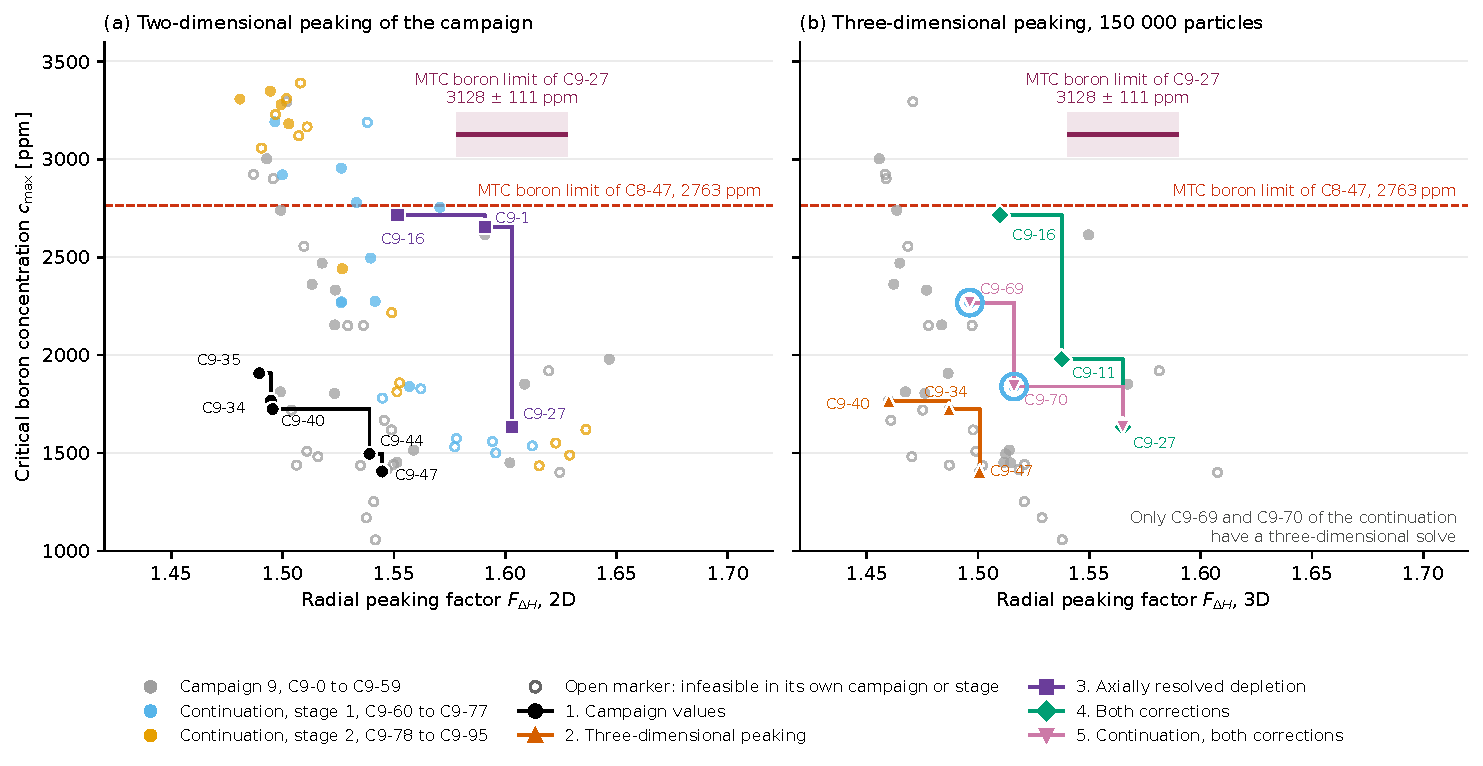
\includegraphics[width=\textwidth]{images/c9_readings}
  \caption{Campaign 9 and its continuation: front under each reading. (a)~Two-dimensional peaking. (b)~Three-dimensional peaking.}
  \label{fig:c9-readings}
\end{figure}

Over every design depleted in 8 layers that satisfies the minimum cycle
length, the non-dominated designs in $(F_{\Delta H}, c_\mathrm{max})$
are C9-27, C9-69 and C9-70, the 3 of Table~\ref{tab:c9-cont-conf} with
a positive margin. C9-69 dominates C9-1, C9-11 and C9-16, the other
members of the corrected front of Section~\ref{sec:res-c9-axial-front},
on both objectives, so the 2 continuation designs replace them.
Table~\ref{tab:c9-final-front} gives the 3 designs with every quantity
measured on them in three dimensions, and the MTC boron limits of C9-69
and C9-70 are those of Section~\ref{sec:res-c9-ceiling}.

\begin{table}[htbp]
  \centering
  \footnotesize
  \begin{threeparttable}
  \caption{Campaign 9, corrected front after the continuation: design variables, objectives and three-dimensional measurements.}
  \label{tab:c9-final-front}
  \setlength{\tabcolsep}{3.6pt}
  \begin{tabular}{@{}lrrrrrrrrrr@{}}
    \toprule
    Design & $e$ & $w_\mathrm{Gd}$ & $n_\mathrm{Gd}$ & $F_{\Delta H}^\mathrm{2D}$ & $F_{\Delta H}^\mathrm{3D}$ & $c_\mathrm{max}$ & $\mathrm{EFPD}_\mathrm{3D}$ & Margin & $c_\mathrm{MTC}$\tnote{a} & MTC margin \\
     & [wt\%] & [wt\%] & & & & [ppm] & [d] & [d] & [ppm] & [ppm] \\
    \midrule
    C9-27 & 5.11 & 5.70 & 24 & 1.603 & 1.565 & 1633 & $1926 \pm 10$\tnote{b} & $+100$ & $3128 \pm 111$\tnote{c} & $+1495$ \\
    C9-69 & 4.87 & 4.38 & 16 & 1.526 & 1.496 & 2268 & $1895 \pm 7$ & $+69$  & $2867 \pm 115$ & $+599$ \\
    C9-70 & 4.87 & 4.41 & 20 & 1.557 & 1.516 & 1840 & $1850 \pm 3$\tnote{b} & $+24$ & $3018 \pm 102$\tnote{c} & $+1178$ \\
    \bottomrule
  \end{tabular}
  \begin{tablenotes}[flushleft]\footnotesize
    \item[a] Three-dimensional core at \SI{12.8}{MPa} (Section~\ref{sec:res-c9-ceiling}).
    \item[b] Mean of 5 seeds and standard error of the mean.
    \item[c] Extrapolated beyond the scanned \SI{3000}{ppm}.
  \end{tablenotes}
  \end{threeparttable}
\end{table}

The final front has four properties:

\begin{itemize}
  \item \textbf{Measured:} every member was depleted in 8 layers, with
        cycle lengths of 1926, 1895 and \SI{1850}{d} and margins of
        100, 69 and \SI{24}{d}, all at least 4 standard errors above
        the minimum.
  \item \textbf{Tested from both sides:} it remained unchanged for
        blocks 10 to 12 under Equation~\eqref{eq:axial-floor}, and the
        2 designs the rule rejected by the smallest margins, C9-85 and
        C9-88, fail when measured, by 36 and \SI{14}{d}.
  \item \textbf{Budget-limited:} stage 1 was still gaining hypervolume
        when it ended and stage 2 spent 10 of its 18 evaluations above
        the MTC boron limit, so a better design under this rule may
        exist in the region the search did not reach.
  \item \textbf{Three-dimensional values:} on the three-dimensional
        core at \SI{1000}{ppm} with 2 seeds, C9-27, C9-69 and C9-70 have
        peaking factors lower than in two dimensions by 0.038, 0.030 and
        0.041, axial leakage factors of 1.030, 1.031 and 1.030 and
        two-bank margins of 6316, 2222 and \SI{4941}{pcm}, and their
        lattices satisfy their own MTC boron limits by 1495, 599 and
        \SI{1178}{ppm}.
\end{itemize}

C9-27 remains the recommended design. It needs the least boron of the
3, \SI{1633}{ppm}, and has the largest cycle margin, \SI{100}{d}. C9-69
and C9-70 offer a lower peaking factor, 1.496 and 1.516 against 1.565
in three dimensions, at 635 and \SI{207}{ppm} more boron and a smaller
cycle margin. The lattice of C9-27 also has the largest margin to its
own MTC boron limit, \SI{1495}{ppm} at \SI{12.8}{MPa}.
Chapter~\ref{ch:conclusions} uses this front.

\section{Sources of uncertainty}
\label{sec:res-uncertainty}\label{sec:res-c9-limits}

The results of Campaigns 8 and 9 are obtained from a model and from Monte Carlo estimates, and the two contribute differently to their uncertainty.
Accuracy is how closely the computed quantities reproduce the physical
core, and it is limited by what the model leaves out. Precision is the
statistical error of the estimates and its propagation through the
post-processing. This section collects both, and Section~\ref{sec:concl-limits}
gives those that affect the conclusions.

\subsection{Accuracy}
\label{sec:res-uncertainty-accuracy}

\begin{enumerate}
  \item \textbf{Dimensionality of the loop model:} every campaign
        evaluates a two-dimensional core at beginning of life,
        corrected for the axial leakage by the measured constant
        $L_\mathrm{ax} = 1.0289$ of Section~\ref{sec:meth-lax}. The
        constant has a systematic uncertainty of \SI{80}{pcm}, and the
        Campaign 9 designs measured in three dimensions are 80 to
        \SI{240}{pcm} above it. The three-dimensional core model
        enters only the post-analyses, where it gives the peaking, the
        bank worths and the axial leakage of the Campaign 8 candidates
        and the Campaign 9 fronts, and where it shows that the leakage
        correction of the unrodded core does not hold for the rodded
        core (Section~\ref{sec:res-kt-burnup}).

  \item \textbf{Axially uniform burnup:} the cycle length of every
        campaign comes from a reflective assembly whose burnup is
        uniform along the height. Depleting the three-dimensional core
        in 8 axial layers shortens the cycle by 12 to 17 per cent
        against a uniform depletion and by 15 to 25 per cent against
        the assembly depletion, removes the margin of both established
        front members, and moves the designs that satisfy the minimum
        cycle length to 4.9 to \SI{5.5}{wt\%}
        (Section~\ref{sec:res-c9-axial}). That depletion keeps the
        temperatures uniform, keeps the boron at \SI{1000}{ppm} and the
        rods withdrawn, and uses one calculation per design, except for
        C9-27, C9-70 and C9-88, which were depleted with 5 seeds.

  \item \textbf{Constant boron:} the depletion is executed at
        \SI{1000}{ppm}, so every cycle length is a lower bound for a
        core operated with boron letdown, and the critical concentration
        is computed at 2 burnup points of the cycle only.

  \item \textbf{Reference fuel loading of $k_\mathrm{target}$:} the
        leakage-corrected end-of-cycle criterion is read from a table
        computed on one reference fuel loading, 4.05 and
        \SI{4.55}{wt\%} without gadolinia, and applied to every design.
        The radial leakage factor decreases with enrichment, by
        $-64 \pm \SI{9}{pcm}$ per wt\% on average and more steeply at
        low enrichment, so $k_\mathrm{target}$ is too high for a design
        of higher enrichment and its reported cycle length is
        conservative, by about 500 to \SI{600}{pcm} at the upper
        enrichment bound of Campaign 8 (Section~\ref{sec:res-kt-burnup}).

  \item \textbf{Controllability constraint:} it tests the
        subcriticality of the rodded core at power with the operating
        boron present and no xenon. It is not a shutdown-margin
        demonstration, which needs the cold state, all assemblies minus
        the highest-worth one, and a stated margin. In Campaigns 1 to 8 the reactivity swing over the cycle was not penalised, and humps of
        several thousand pcm appear in the depletion histories.
        Campaign 9 applies the constraint at the operating maximum and
        closes this point for the last campaign only.

  \item \textbf{Thermal-hydraulic feedback:} it is absent. Temperatures
        are fixed at representative hot full power values, so no
        departure from nucleate boiling ratio and no fuel temperature
        limit is evaluated. The moderator temperature coefficient was
        evaluated outside the loop, on the lattice of C8-47 and on 11
        Campaign 9 lattices at \SI{12.8}{MPa}, 8 of them also at
        \SI{15.5}{MPa}, and enters only through the MTC boron limit. The
        limit increases with the gadolinia loading, but the lattices
        confound that loading with the reflector thickness, which is at
        its bound for 10 of the 11, so the fitted relation holds only
        inside the converged region of Campaign 9 and the limit of any
        other lattice has to be measured. C9-58 clears its own limit by
        \SI{120}{ppm} only.

  \item \textbf{Discharge-burnup limit:} the limit of \SI{55}{MWd/kgHM}
        of Section~\ref{sec:meth-atf} acts on the assembly-average
        burnup. The burnup of the most loaded rod, to which fuel
        performance limits apply, is higher by the radial power
        peaking, and no constraint of the problem limits it. The effect
        is largest for the long-cycle designs of Campaign 8, C8-44 and
        C8-59, which reach about 50 and \SI{51}{MWd/kgHM} on average,
        and small for the Campaign 9 designs, whose most loaded ring
        stays below \SI{23}{MWd/kgHM}.
        %% AUTHOR: state the fuel-performance basis you adopt for the
        %% discharge burnup and whether it removes C8-44 and C8-59 from
        %% the candidate list.

  \item \textbf{Geometry of the early campaigns:} every design below a
        pitch of \SI{1.224}{cm} in Campaigns 1 to 7 carried truncated
        guide tubes. Campaigns 8 and 9 are free of the defect and the
        earlier results are qualified by it.

  \item \textbf{Deviations from the reference specification:} 2
        values adopted in the campaign model were checked against it on
        C8-21 and C8-47. The reflector steel fraction of 0.90, against
        0.956, makes the model conservative by 182 to \SI{199}{pcm},
        and the absorber radius of \SI{0.433}{cm}, against
        \SI{0.423}{cm}, raises the four-bank worth by 131 to
        \SI{169}{pcm}. The deviation of the coolant density was not
        quantified.

  \item \textbf{Boundary optimum:} every front member of Campaign 9 has
        the largest reflector the vessel admits, a bound the optimiser
        reached in the first infill iteration and never left, so the
        front is conditional on the vessel envelope and the clearance
        of Section~\ref{sec:meth-c8-space}.
\end{enumerate}

\subsection{Precision}
\label{sec:res-uncertainty-precision}

\begin{enumerate}
  \item \textbf{Cycle length:} the seed replicates of
        Section~\ref{sec:res-c9-dep-check} measure a statistical error
        of \SI{29.1}{d} on the assembly cycle length at the setting of
        the search, 1.33 times the value
        propagated from the two depletion steps, and the eight-layer
        cycle length, replicated with 5 seeds on C9-27, C9-70 and C9-88,
        has a seed standard deviation of \SI{15.1}{d}, 1.74 times the
        propagated value. Two
        members of the campaign front, C9-40 and C9-44, are \SI{6}{d}
        below the minimum cycle length over 9 samples each, inside
        one standard error of \SI{9.7}{d}, and no cycle-length
        feasibility is claimed for them. Separating a \SI{6}{d} margin
        from zero at 2 standard errors would need about 90
        replicates per design. On the final front the smallest margin,
        \SI{24}{d} of C9-70, is 7.8 standard errors of its 5-seed mean.

  \item \textbf{Peaking factor:} the single-solve standard deviation is
        0.011 on the Campaign 8 designs at the confirmation statistics
        and 0.012 on the Campaign 9 front at the campaign statistics,
        where the core estimator also carries an upward bias of
        $+0.060$ to $+0.077$ that varies by 0.017 between front
        designs. Five of the 10 pairs of the Campaign 9 front are not
        statistically distinguishable by one campaign solve, the
        three-dimensional value changes which designs are
        non-dominated, and Table~\ref{tab:c9-front} is therefore a list
        of comparable designs rather than an ordered ranking
        (Section~\ref{sec:res-c9-peaking}).

    \item \textbf{Stability of the campaign front:} only C9-47 and C9-34
        remain on the front in at least 99 per cent of the resamples of
        Table~\ref{tab:c9-stability}. When the campaign values are
        perturbed by their statistical error, the front recomputed on
        the perturbed values has on average a hypervolume
        \SI{3.7}{\%} larger than the front of the campaign values, so a
        front selected on single noisy evaluations overestimates its own
        hypervolume by about that amount. The bias applies to the front
        of the campaign values and not to the final front of
        Section~\ref{sec:res-c9-cont-front}, whose members are measured
        with replicates and in three dimensions.

  \item \textbf{MTC boron limit:} the uncertainty of each limit is that
        of the three-point fit, 53 to \SI{240}{ppm}, 3 of the
        19 Campaign 9 scans have $\chi^2/\nu$ above 2, and the
        limits of C9-70 and C9-27 at both pressures and of C9-69 at
        \SI{15.5}{MPa} are extrapolated beyond the scanned
        \SI{3000}{ppm}. The quoted margins combine a three-dimensional
        limit with a two-dimensional concentration and are conservative
        by about \SI{450}{ppm} (Section~\ref{sec:res-c9-ceiling}).

  \item \textbf{Acquisition and reproducibility:} with the cycle-length
        constraint active on the front, no candidate passed the
        feasibility margin and every batch came from the fallback
        ordering (Table~\ref{tab:c9-acq-health}), so the batches were
        selected by confidence in the predicted cycle length rather than
        for exploration. The design of experiments of every campaign
        was sampled without a fixed seed, so a campaign is reproducible
        from its stored results and not from its launch settings, and
        the depletion itself is reproduced only within its statistical
        error (Section~\ref{sec:meth-fid-seed}).
\end{enumerate}

Three of these sources were tested for their effect on the campaign
front. The MTC boron limit of each lattice
(Section~\ref{sec:res-c9-ceiling}) accepts every member of that front.
The three-dimensional peaking factor (Section~\ref{sec:res-c9-peaking})
changes the membership of the front but keeps C9-47, its best-ranked
design, non-dominated. The axially resolved depletion
(Section~\ref{sec:res-c9-axial}) places C9-47 and C9-35 below the
minimum cycle length, so it is the one source that changes a
conclusion. After the continuation of the search, the front is C9-27,
C9-69 and C9-70, and the recommended design is C9-27.

\setcounter{secnumdepth}{2}
